\documentclass[a4paper, 10pt, english]{article}
\usepackage[utf8]{inputenc}
\usepackage[total={6.69in, 10in}]{geometry}
\usepackage[english]{babel}
\usepackage{silence}
\WarningFilter{latex}{File `}
\WarningFilter{latex}{Package}
% \newcommand{\sectionbreak}{\clearpage}
\hbadness=10000
\vbadness=10000
\usepackage{microtype}
\usepackage{collcell}
\usepackage{etoolbox}
\usepackage{xstring}
\usepackage{lipsum}
\usepackage{listings}

\usepackage{tikz, ifthen, xstring, calc, pgfopts}
\usepackage{pgf-umlcd}
\usepackage[ruled,linesnumbered]{algorithm2e}
% %\usepackage{algorithm}
% %\usepackage{algpseudocode} %% Algorithms is this ok Roni?
\usepackage{tikz} %%% Plot graphs 
\usetikzlibrary{shapes,decorations,arrows,calc,arrows.meta,fit,positioning}
\usepackage{todonotes}
\usepackage{fancyhdr}
\usepackage{enumerate}
\usepackage[hyphens]{url}
\urlstyle{same}
\usepackage{url}
% \def\UrlBreaks{\do\/\do-}
% \usepackage{breakurl}
\usepackage{blindtext}

\usepackage{pdfpages}
\usepackage{csvsimple}
% \usepackage{subfig}
% \usepackage{subfigure}
\usepackage{bookmark}
\usepackage{setspace}
\usepackage{reledmac}
\usepackage{setspace}
\usepackage{microtype}
% \usepackage{etoolbox}
% \usepackage{etool}
% \usepackage{dblfnote}
% \usepackage{ftnright}
% \arrangementX[A]{twocol}
% % \colalignX{\justifying}
% \makeatletter
% \bhooknoteX[A]{\setstretch{1}}
% \bhookgroupX[A]{\setstretch{1}}
% \makeatother
% \let\footnote\footnoteA
\usepackage{datatool}
% \usepackage[bookmarksnumbered]{hyperref} %add hidelinks evt
\usepackage[capitalise, noabbrev]{cleveref}
\crefdefaultlabelformat{#2\textbf{#1}#3}
\newcounter{RQ}
\renewcommand{\theRQ}{\textbf{\arabic{RQ}}}
\crefname{RQ}{RQ}{RQs}
%\crefformat{RQ1}{\textbf{RQ1}}
%\crefformat{RQ2}{\textbf{RQ2}}
%\crefformat{RQ3}{\textbf{RQ3}}
%\crefformat{RQ4}{\textbf{RQ4}}
\crefname{subsec}{subsection}{subsections}
\Crefname{subsec}{Subsection}{Subsections}
\usepackage{hyperref}

\usepackage{graphicx}
\usepackage{pgf-pie} %%% make pies 
\usepackage{pgfplots} %%% PLOT THAT SHITTS
\usepgfplotslibrary{statistics}
\usepackage{pgfplotstable}
\pgfplotsset{compat=1.14}
\usepackage{wrapfig}
\usepackage[labelfont=bf]{caption}
%\captionsetup[figure]{font=small}
\usepackage{indentfirst}
\usepackage{subcaption}
\graphicspath{ {./Figures/} }
%Table packages
\usepackage{longtable}
\usepackage{amsmath, tabu, centernot}
\newcommand{\bigCI}{\mathrel{\text{\scalebox{1.07}{$\perp\mkern-10mu\perp$}}}}
\newcommand{\nbigCI}{\centernot{\bigCI}}
\usepackage{xcolor,colortbl}
\usepackage[export]{adjustbox}
\usepackage{multirow}
\usepackage{multicol}
\usepackage{float}
\usepackage{changepage} %% indents paragrahs with \adjustwidth 
\usepackage{array}
%table text size
\usepackage{pdfpages}
\usepackage{bbding} %%%% Add icons like checkmars with command: \Checkmark
%%\usepackage{stmaryrd} %%%% Add icons like arrows 
%%\usepackage{mathabx} %%%% Add math icons 
%TOC 
\usepackage{titlesec}
\usepackage[titletoc]{appendix}
% \titleformat{\chapter}[display]
%   {\normalfont\bfseries}{}{10pt}{\Huge\thechapter.\quad}
%Vis sidetal
\usepackage{lastpage}
%font
\usepackage[sc]{mathpazo}
\linespread{1.05} 
% load a colour package
% \usepackage{xcolor}
\definecolor{aaublue}{RGB}{33,26,82}% dark blue
% Make the standard latex tables look so much better
\usepackage{array,booktabs}
% Enable the use of frames around, e.g., theorems
% The framed package is used in the example environment
\usepackage{framed}
% Defines new environments such as equation,
% align and split 
\usepackage{amsmath}
\usepackage{mathtools}
% Adds new math symbols
\usepackage{amssymb}
% Use theorems in your document
% The ntheorem package is also used for the example environment
% When using thmmarks, amsmath must be an option as well. Otherwise \eqref doesn't work anymore.
\usepackage[amsmath,thmmarks]{ntheorem}
%lav afsnit med denne commando
\newcommand{\nytafsnit}{\newline\newline \indent}


\usepackage[giveninits=true, backend = biber, style=nature]{biblatex}
\usepackage{hyphenat}

\bibliography{bib.bib}

\usepackage{csquotes}
\newtheorem{theorem}{Theorem} 
\newtheorem{definition}{Definition}
% \newtheorem{lemma}{Lemma}

\titleformat{\chapter}{}{}{0em}{\bfseries\LARGE\ifnum\value{chapter}>0\relax\arabic{chapter}.~\f}
\usepackage{dblfnote}
\pretocmd{\footnote}{%
  \widowpenalty=150% LaTeX default value
}{}{}

\newcolumntype{T}{>{\columncolor{Gray}}c}
\newcolumntype{Q}{>{\columncolor{white}}c}
\newcolumntype{Z}{>{\columncolor{DarkGray}}c}

\titleformat{\subsubsection}[runin]{\bfseries}{}{}{}[.]
\definecolor{codegreen}{rgb}{0,0.6,0}
\definecolor{codegray}{rgb}{0.5,0.5,0.5}
\definecolor{codepurple}{rgb}{0.58,0,0.82}
\definecolor{backcolour}{rgb}{0.95,0.95,0.92}

\lstdefinestyle{csharp_style}{
    backgroundcolor=\color{backcolour},   
    commentstyle=\color{codegreen},
    keywordstyle=\color{magenta},
    numberstyle=\tiny\color{codegray},
    stringstyle=\color{codepurple},
    basicstyle=\ttfamily\footnotesize,
    breakatwhitespace=false,         
    breaklines=true,                 
    captionpos=b,                    
    keepspaces=true,                 
    numbers=left,                    
    numbersep=8pt,                  
    showspaces=false,                
    showstringspaces=false,
    showtabs=false,                  
    tabsize=2,
    frame=lines,
    %linewidth=0.9\linewidth, % Set the width of the listing to 90% of the current line width
    xleftmargin=0.05\linewidth,
}

\colorlet{punct}{red!60!black}
\definecolor{background}{HTML}{EEEEEE}
\definecolor{delim}{RGB}{20,105,176}
\colorlet{numb}{magenta!60!black}

\lstdefinelanguage{json}{
    % basicstyle=\normalfont\ttfamily,
    basicstyle=\ttfamily\footnotesize,
    numbers=left,
    % numberstyle=\scriptsize,
    numberstyle=\tiny\color{codegray},
    stepnumber=1,
    numbersep=8pt,
    showstringspaces=false,
    breaklines=true,
    frame=lines,
    backgroundcolor=\color{backcolour},
    literate=
     *{0}{{{\color{numb}0}}}{1}
      {1}{{{\color{numb}1}}}{1}
      {2}{{{\color{numb}2}}}{1}
      {3}{{{\color{numb}3}}}{1}
      {4}{{{\color{numb}4}}}{1}
      {5}{{{\color{numb}5}}}{1}
      {6}{{{\color{numb}6}}}{1}
      {7}{{{\color{numb}7}}}{1}
      {8}{{{\color{numb}8}}}{1}
      {9}{{{\color{numb}9}}}{1}
      {:}{{{\color{punct}{:}}}}{1}
      {,}{{{\color{punct}{,}}}}{1}
      {\{}{{{\color{delim}{\{}}}}{1}
      {\}}{{{\color{delim}{\}}}}}{1}
      {[}{{{\color{delim}{[}}}}{1}
      {]}{{{\color{delim}{]}}}}{1},
}
\begin{document}
\newpage
\title{\huge Exploring the Energy Consumption of Highly Parallel  Software on Windows}
\author{
Mads Hjuler Kusk*, Jeppe Jon Holt*\\ and Jamie Baldwin Pedersen*\\
\texttt{Department of Computer Science, Aalborg University, Denmark}\\
*\texttt{$\text{\{mkusk18, jholt18, jjbp18\}@student.aau.dk}$}
}

% \begin{figure}[H]
    \centering
\begin{tikzpicture}
    \pgfplotsset{
        width=1.0\textwidth,
        height=0.25\textheight
    }
    \begin{axis}[
        xlabel={Time (s)},
        ylabel={Energy Consumption (w)},
        xmin=0,%, xmax=80,
        ymin=6, ymax=12,
        legend pos=north west,
        ymajorgrids=true,
        grid style=dashed,
    ]
    
    \addplot[
        color=blue,
        % mark=square,
        ]
        coordinates {
            (0.8635000387827567, 9.966875036557516)
            (0.9742498397827148, 10.3681667248408)
            (1.0855002403259277, 10.459124942620596)
            (1.1947917938232422, 10.464041610558828)
            (1.3040835062662772, 9.400916695594788)
            (1.4126666386922189, 9.136874973773956)
            (1.5214584668477364, 9.276500006516775)
            (1.6346250375111886, 9.080458303292593)
            (1.7436248461405448, 9.48758331934611)
            (1.8540833791096993, 9.636041641235352)
            (1.9631249904632568, 9.062166631221771)
            (2.0734167098999023, 9.279208342234293)
            (2.184333324432373, 8.895666718482971)
            (2.296958367029827, 8.420458296934763)
            (2.4048333168029785, 7.648041665554047)
            (2.5154585043589286, 7.720249990622203)
            (2.626875003178913, 7.957833329836528)
            (2.7380417188008614, 7.998500009377797)
            (2.8492497603098563, 7.973916669686635)
            (2.9587916533152274, 8.016833364963531)
            (3.069749991099041, 7.990708351135254)
            (3.181416591008503, 8.301041583220163)
            (3.2922081152598075, 7.939708332220714)
            (3.4016249974568673, 8.028083423773447)
            (3.5122917493184396, 8.18241661787033)
            (3.6238749821980782, 8.449625035127005)
            (3.7337085405985526, 8.442250033219656)
            (3.8450833956400565, 8.241958340009054)
            (3.954708258310955, 8.259541610876719)
            (4.066208362579346, 8.345375061035156)
            (4.1760419209798165, 8.320291658242544)
            (4.285999933878582, 8.286083360513052)
            (4.396458148956299, 8.310791770617167)
            (4.507708390553791, 8.458624998728434)
            (4.6194167137146, 8.531083345413208)
            (4.73074968655904, 8.370333234469095)
            (4.8418333530426025, 8.450291633605957)
            (4.9527916113535575, 8.355583369731903)
            (5.062791585922241, 8.286916732788086)
            (5.1739583015441895, 8.327583372592926)
            (5.285125017166138, 8.165416618188223)
            (5.3956252733866386, 8.18358333905538)
            (5.506708383560181, 8.185291667779287)
            (5.618208249409992, 8.303499937057495)
            (5.727708260218304, 8.34870833158493)
            (5.838708400726318, 8.184166769186655)
            (5.950416644414265, 8.106374979019165)
            (6.061958312988281, 8.122999926408133)
            (6.172791639963787, 8.150958319505056)
            (6.284250020980835, 8.234041631221771)
            (6.394374926884968, 8.142291605472565)
            (6.505916674931843, 8.125374992688497)
            (6.616208235422771, 8.098833362261454)
            (6.727083285649616, 8.077958305676779)
            (6.837416728337605, 8.07179162899653)
            (6.94895847638448, 8.054583311080933)
            (7.059958457946777, 8.042125046253204)
            (7.170499960581463, 8.050833284854889)
            (7.28066651026408, 8.235041558742523)
            (7.3916250069936105, 8.066750089327494)
            (7.502791802088421, 8.026166697343191)
            (7.613208293914795, 7.9726666410764055)
            (7.725000063578289, 8.04562497138977)
            (7.83637507756551, 8.020583291848501)
            (7.94770844777425, 8.074666659037272)
            (8.058250188827515, 8.02420828739802)
            (8.16975005467733, 8.081375002861023)
            (8.279416720072426, 8.01108326514562)
            (8.389666557312012, 8.048125008742014)
            (8.500624974568687, 7.984374980131785)
            (8.611749966939293, 7.975333313147227)
            (8.721333344777427, 8.003124932448069)
            (8.831833203633629, 8.00695832570394)
            (8.943666776021324, 7.912666658560435)
            (9.055250008900963, 8.029874980449677)
            (9.165875116984047, 8.109708348910013)
            (9.27708307902018, 8.081125020980835)
            (9.387833277384438, 8.09333332379659)
            (9.497458457946777, 7.979208330313365)
            (9.609249909718834, 8.054833372433981)
            (9.720416386922203, 8.101333399613699)
            (9.832291444142662, 8.015750030676523)
            (9.942124843597412, 8.077666640281677)
            (10.054000059763588, 8.043041626612345)
            (10.165583610534668, 8.03333338101705)
            (10.278250217437744, 8.044333259264628)
            (10.38908338546753, 8.028958400090536)
            (10.500791708628334, 8.019916633764902)
            (10.611292044321694, 8.218374927838644)
            (10.722291946411133, 8.116458376248678)
            (10.833916664123535, 8.062333345413208)
            (10.944958209991455, 8.16070830821991)
            (11.056124846140541, 8.069791654745737)
            (11.168083349863686, 8.093208332856497)
            (11.276916980743408, 8.115499953428904)
            (11.38683350880941, 8.142458339532217)
            (11.497833887736, 8.059374968210856)
            (11.608875115712486, 8.065541644891104)
            (11.71879164377848, 8.018875002861023)
            (11.829625129699707, 7.942125022411346)
            (11.941374937693276, 7.855624993642171)
            (12.05174970626831, 7.893666664759318)
            (12.162291526794434, 8.002166668574015)
            (12.27254136403402, 8.174333413441977)
            (12.384083588918052, 8.190041561921438)
            (12.49466689427694, 8.266333242257437)
            (12.606458346048989, 8.185500045617422)
            (12.717374801635742, 8.18241661787033)
            (12.827875137329102, 8.214541733264923)
            (12.938875198364258, 8.104375064373016)
            (13.05045827229818, 8.12270841995875)
            (13.161333401997886, 8.144666711489359)
            (13.271958351135254, 8.34579167763392)
            (13.381291389465332, 8.317416628201803)
            (13.49237505594889, 8.281833370526632)
            (13.604041576385498, 8.231291651725769)
            (13.715125242869057, 8.313125014305115)
            (13.826999982198082, 8.408708254496256)
            (13.938791751861572, 8.316583255926767)
            (14.048583666483559, 8.383416593074799)
            (14.161125183105469, 8.498374978701273)
            (14.271250089009605, 8.597208360830942)
            (14.38083346684774, 8.694583336512247)
            (14.492000102996826, 8.579500019550323)
            (14.603041489919029, 8.649875005086264)
            (14.713958263397217, 8.61020827293396)
            (14.82545804977417, 8.681666811307272)
            (14.935832818349205, 8.724416772524515)
            (15.046874682108559, 8.720333397388458)
            (15.159083366394043, 8.710125029087067)
            (15.268625100453697, 8.771999994913736)
            (15.37916692097982, 9.27833334604899)
            (15.490125179290771, 9.464166839917501)
            (15.601083278656006, 9.157916784286499)
            (15.711708386739097, 8.94000001748403)
            (15.822458267211914, 8.876874923706055)
            (15.93329175313314, 8.94795842965444)
            (16.045124848683677, 8.855416655540466)
            (16.157541751861572, 8.9437917470932)
            (16.266958554585777, 8.969791690508524)
            (16.376625219980873, 8.951500097910563)
            (16.487625122070312, 9.039874990781149)
            (16.599250157674156, 8.989458401997885)
            (16.71083323160807, 8.93133314450582)
            (16.821916262308754, 8.867833296457926)
            (16.932374954223633, 9.26604163646698)
            (17.044083436330162, 9.327916622161865)
            (17.15662511189779, 8.90304164091746)
            (17.266458193461098, 8.980291604995728)
            (17.376208464304604, 9.079750061035156)
            (17.48770840962728, 8.990958372751871)
            (17.599416732788086, 8.877458333969116)
            (17.710458437601723, 8.845541735490164)
            (17.821458180745445, 8.851791620254517)
            (17.932041327158608, 8.803416768709818)
            (18.04366683959961, 8.765999933083853)
            (18.15616718928019, 8.631083369255066)
            (18.26679197947184, 8.61816664536794)
            (18.37575054168701, 8.69575003782908)
            (18.486375331878662, 8.668708364168802)
            (18.59754180908203, 8.602916677792868)
            (18.70924997329712, 8.554916659990946)
            (18.820499897003174, 8.696208397547403)
            (18.930250008900963, 8.784791648387909)
            (19.0412917137146, 9.242666721343994)
            (19.153499921162926, 9.356916546821594)
            (19.26237519582113, 9.257791618506113)
            (19.37404155731201, 9.079333384831747)
            (19.483749866485596, 9.142500003178915)
            (19.595291455586754, 8.763166666030884)
            (19.705708344777427, 8.603750069936117)
            (19.81599966684977, 8.733083268006643)
            (19.927500089009605, 9.175291617711386)
            (20.03808355331421, 8.878041704495748)
            (20.150041898091636, 8.960208257039389)
            (20.264333724975586, 9.300166666507721)
            (20.36970853805542, 9.000500003496805)
            (20.481458504994713, 8.924958348274231)
            (20.593416690826416, 9.348750015099844)
            (20.70229196548462, 8.86641671260198)
            (20.81379191080729, 9.049499948819479)
            (20.925874869028725, 9.06633327404658)
            (21.036374727884926, 9.040083309014639)
            (21.148541132609047, 8.969583292802175)
            (21.259291807810463, 9.286666711171469)
            (21.371125062306724, 8.86508329709371)
            (21.479332764943443, 8.879541655381521)
            (21.59266678492228, 9.162791649500528)
            (21.70124944051107, 8.835624972979227)
            (21.813416798909508, 8.626541674137115)
            (21.92399994532267, 8.949458281199137)
            (22.035916805267334, 8.676791568597158)
            (22.149083296457924, 8.673041701316833)
            (22.259666760762535, 8.882624944051107)
            (22.371749877929688, 8.777458329995474)
            (22.4816247622172, 8.503166635831198)
            (22.593249797821045, 8.89600016673406)
            (22.704166889190674, 8.606291671593985)
            (22.815249919891357, 8.592875023682913)
            (22.92533334096273, 8.664374927679697)
            (23.036333401997886, 8.689458350340525)
            (23.14833354949951, 8.46958327293396)
            (23.26020860671997, 8.78966655333837)
            (23.370625178019203, 8.70695831378301)
            (23.481416702270508, 8.57141669591268)
            (23.591749827067055, 8.631374994913736)
            (23.70349963506063, 8.717874924341837)
            (23.814666271209717, 8.437041699886322)
            (23.926208337148033, 8.603416621685028)
            (24.037083307902016, 8.714666684468588)
            (24.14883327484131, 8.607541700204214)
            (24.2605832417806, 8.635916610558828)
            (24.37124983469645, 9.051291624704996)
            (24.480916500091553, 8.624708314736685)
            (24.59162473678589, 8.781249940395355)
            (24.702583471934, 9.032791753609976)
            (24.81391684214274, 8.569791714350382)
            (24.924999872843422, 8.465708335240683)
            (25.035249869028725, 8.83404165506363)
            (25.145750045776367, 8.568166653315226)
            (25.25829188028971, 8.4280832807223)
            (25.36858320236206, 8.718000054359436)
            (25.47891664505005, 8.759708325068155)
            (25.59025001525879, 8.474999964237213)
            (25.70179192225138, 8.675749997297922)
            (25.812791665395103, 8.747500002384186)
            (25.924416542053223, 8.417666713396708)
            (26.03550020853678, 8.377083341280619)
            (26.146083513895668, 8.633083403110504)
            (26.257374922434487, 8.483791728814444)
            (26.36866648991903, 8.479874968528748)
            (26.480249881744385, 8.879083236058554)
            (26.590541998545326, 8.510374983151754)
            (26.70087512334188, 8.495124995708466)
            (26.81124989191691, 8.409625033537546)
            (26.9229998588562, 8.71329172452291)
            (27.034625371297203, 8.264958361784617)
            (27.145083268483482, 8.424833317597708)
            (27.257750193277992, 8.907416661580404)
            (27.367458184560142, 8.491041660308838)
            (27.478500048319496, 8.523541649182638)
            (27.588875134785972, 8.431416670481363)
            (27.700750033060707, 8.675083259741465)
            (27.811666647593178, 8.19950004418691)
            (27.922749996185303, 8.637041628360748)
            (28.033083756764732, 8.71304170290629)
            (28.14400005340576, 8.503708362579346)
            (28.256208419799805, 8.455833276112875)
            (28.36554193496704, 8.641000012556711)
            (28.475250244140625, 8.599749883015951)
            (28.584999879201256, 8.368499974409739)
            (28.695374806722008, 8.76779160896937)
            (28.806999842325844, 8.615125000476837)
            (28.91891622543335, 8.56395826737086)
            (29.03054110209147, 8.400250017642975)
            (29.14224942525228, 8.696041564146677)
            (29.25425020853678, 8.43979169925054)
            (29.36533339818319, 8.436791777610779)
            (29.4768754641215, 8.897333363691965)
            (29.588750521341957, 8.742708345254263)
            (29.70020834604899, 8.447583258152008)
            (29.8119166692098, 8.369124948978424)
            (29.923833211263023, 8.875125030676523)
            (30.03454144795736, 8.351999998092651)
            (30.1442502339681, 8.537833313147226)
            (30.25695832570394, 8.867041607697805)
            (30.36608362197876, 8.561541775862375)
            (30.478041807810463, 8.671541651089987)
            (30.588791529337563, 8.435000002384186)
            (30.699833393096924, 8.85979167620341)
            (30.811624685923256, 8.321458399295807)
            (30.92183335622152, 8.676541725794474)
            (31.03312508265177, 8.798916697502136)
            (31.144458611806236, 8.569374958674112)
            (31.25675026575724, 8.568958342075348)
            (31.367666721343994, 8.584874947865805)
            (31.47920846939087, 8.751458366711935)
            (31.589916229248047, 8.451666812102)
            (31.698791662851967, 9.047250072161356)
            (31.809666315714516, 8.726375043392181)
            (31.92124970753988, 8.584874967734018)
            (32.03249979019165, 8.489333311716715)
            (32.143041451772056, 8.702333311239878)
            (32.253499825795494, 8.547249972820282)
            (32.365125020345054, 8.4594167470932)
            (32.47641706466675, 8.87045830488205)
            (32.586458683013916, 8.572291612625122)
            (32.69833358128866, 8.522166669368744)
            (32.81008338928223, 8.38720840215683)
            (32.92112477620443, 8.708041648070017)
            (33.03166643778483, 8.407666623592377)
            (33.14324935277303, 8.75558336575826)
            (33.255040963490806, 9.051083385944366)
            (33.36570771535238, 8.757458408673605)
            (33.47637494405111, 8.718166708946228)
            (33.58779191970825, 8.70620838801066)
            (33.69970893859863, 8.847499986489614)
            (33.809833685557045, 8.516249974568685)
            (33.92145872116089, 8.792333344618479)
            (34.03175004323324, 8.7293750445048)
            (34.142333348592125, 8.56800001859665)
            (34.25245841344198, 8.655458291371664)
            (34.36420822143555, 8.719416598478952)
            (34.47483332951864, 8.723666608333588)
            (34.58654165267944, 8.419624964396158)
            (34.696999867757164, 9.001708328723907)
            (34.807416915893555, 8.679541607697805)
            (34.918458779652916, 8.602916657924652)
            (35.029541969299316, 8.514124989509583)
            (35.1409584681193, 8.671000083287558)
            (35.25295845667521, 8.462875028451284)
            (35.36508321762085, 8.58433336019516)
            (35.47504154841105, 8.810958305994669)
            (35.58591604232788, 8.540791630744934)
            (35.69762452443441, 8.501583357652029)
            (35.80954202016195, 8.42662501335144)
            (35.920125325520836, 8.57287492354711)
            (36.03195858001709, 8.381750027338663)
            (36.14237483342489, 8.642666657765707)
            (36.25320831934611, 8.832708378632864)
            (36.36366637547811, 8.695541540781656)
            (36.47458299001058, 8.725083390871683)
            (36.58579142888387, 8.518416702747345)
            (36.69683297475179, 8.476750016212463)
            (36.80775022506714, 8.503624876340231)
            (36.919458548227944, 8.790083467960358)
            (37.02999989191691, 8.53012502193451)
            (37.14179197947184, 8.445416649182638)
            (37.25354162851969, 8.642291684945425)
            (37.36433331171671, 8.702791611353556)
            (37.47508319218954, 8.47104169925054)
            (37.58579158782959, 8.57387493054072)
            (37.69683313369751, 8.908166607220968)
            (37.807083447774254, 8.612250129381815)
            (37.91729164123535, 8.583125034968058)
            (38.02841647466024, 8.603750069936117)
            (38.140666802724205, 8.500499963760376)
            (38.25191672643026, 8.43862501780192)
            (38.36358324686686, 8.865416725476583)
            (38.47375011444092, 8.73408337434133)
            (38.58483346303304, 8.476666649182638)
            (38.69545841217041, 8.801416595776876)
            (38.80620813369751, 8.747458358605703)
            (38.91570854187012, 8.462916612625122)
            (39.02666695912679, 8.401291688283285)
            (39.13850005467733, 8.878875017166138)
            (39.24999984105428, 8.572791735331217)
            (39.361208279927574, 8.693291743596395)
            (39.47141647338867, 8.90679164727529)
            (39.582874615987144, 8.445874949296316)
            (39.69433307647705, 8.515249967575073)
            (39.80404154459635, 8.904041628042856)
            (39.91566642125448, 8.742791632811228)
            (40.02604166666667, 8.454125006993612)
            (40.13691695531209, 8.748291750748953)
            (40.24854167302449, 8.607708394527435)
            (40.358958085378006, 8.509208261966705)
            (40.46933301289876, 8.874916712443033)
            (40.579750061035156, 8.82212487856547)
            (40.69070911407471, 8.449041624863943)
            (40.80254205067952, 8.739291687806448)
            (40.9142500559489, 8.679958244164785)
            (41.02545801798503, 8.467375000317892)
            (41.137874603271484, 8.682874977588654)
            (41.248583157857254, 8.862874984741211)
            (41.35891660054524, 8.505083322525024)
            (41.46995862325032, 8.852041562398275)
            (41.58133316040039, 8.80016678571701)
            (41.6931250890096, 8.462916533152262)
            (41.804000218709305, 8.752791742483774)
            (41.91449960072835, 8.871624986330668)
            (42.02508322397868, 8.758958399295807)
            (42.13666693369548, 8.834458390871683)
            (42.24737485249837, 9.00670838356018)
            (42.359749476114914, 8.70020842552185)
            (42.47029145558675, 8.900541762510935)
            (42.58112462361653, 8.827999949455261)
            (42.69333267211914, 8.724458316961924)
            (42.803500175476074, 8.951416730880737)
            (42.915208498636886, 8.813250064849854)
            (43.02637481689453, 8.67074998219808)
            (43.13904158274333, 8.860458334287008)
            (43.24949963887532, 8.807125131289164)
            (43.36087481180827, 8.81683341662089)
            (43.47099939982097, 8.942416648070017)
            (43.58212534586589, 8.838041643301645)
            (43.69325002034505, 8.734291712443033)
            (43.803583780924484, 8.79791667064031)
            (43.91475073496501, 8.829124927520752)
            (44.02579212188721, 8.637375076611837)
            (44.13741683959961, 8.931500097115835)
            (44.24862575531006, 8.835291743278503)
            (44.35945796966553, 8.766916731993357)
            (44.46979173024495, 8.808999995390574)
            (44.580083529154464, 8.852458278338114)
            (44.69116687774658, 8.725333333015442)
            (44.802458445231125, 8.895874996980032)
            (44.912458419799805, 8.837916652361551)
            (45.024291674296066, 8.647708217302958)
            (45.13570849100749, 8.62612497806549)
            (45.24462445576985, 8.92662501335144)
            (45.35574944814046, 8.74141663312912)
            (45.467749277750656, 9.048666656017303)
            (45.57833290100098, 8.851999998092651)
            (45.68904113769531, 8.704291661580404)
            (45.801290829976395, 8.654583315054575)
            (45.91262435913086, 8.88949998219808)
            (46.02224985758464, 8.719916621843973)
            (46.13387521107991, 8.850000063578287)
            (46.24458312988281, 8.804541647434235)
            (46.354667345682785, 8.58383329709371)
            (46.46612548828125, 8.571875075499216)
            (46.57729212443034, 8.842125018437704)
            (46.68887583414714, 8.762458284695944)
            (46.800667126973465, 8.981875042120615)
            (46.91041692097981, 8.823750058809916)
            (47.021749814351395, 8.675041576226553)
            (47.13329219818115, 8.450166583061218)
            (47.244208335876465, 8.724166750907898)
            (47.35604127248128, 8.62583339214325)
            (47.467749277750656, 8.957166691621145)
            (47.57883294423421, 8.985999941825867)
            (47.6904993057251, 8.611166695753733)
            (47.80141607920329, 8.644624968369802)
            (47.91070874532063, 8.831625044345856)
            (48.021333376566574, 8.785458266735077)
            (48.1326249440511, 8.846458295981089)
            (48.24287509918213, 8.918166677157084)
            (48.355000495910645, 8.549708406130472)
            (48.46587562561035, 8.479041695594788)
            (48.57612546284993, 8.855999986330668)
            (48.68716684977214, 8.791958371798197)
            (48.79879220326741, 8.452333370844523)
            (48.909333546956375, 8.900666654109955)
            (49.019792556762695, 8.56124997138977)
            (49.132083892822266, 8.56387492020925)
            (49.2427921295166, 8.64879161119461)
            (49.354791959126786, 8.764541645844778)
            (49.4652083714803, 8.555291732152304)
            (49.575666427612305, 8.914999882380167)
            (49.68754132588704, 8.941916704177856)
            (49.79762490590413, 8.555208484331766)
            (49.90816593170166, 8.355749984582266)
            (50.01891613006592, 8.830874860286713)
            (50.13041591644287, 8.724750101566315)
            (50.24191633860271, 8.718208332856497)
            (50.353916486104325, 8.892875015735626)
            (50.463540712992355, 8.496625045935312)
            (50.57412465413411, 8.529624978701273)
            (50.68599955240886, 8.857624967892965)
            (50.79720846811931, 8.699833373228708)
            (50.90808327992757, 8.358374993006388)
            (51.01879183451335, 8.918166637420654)
            (51.13000011444092, 8.625874976317087)
            (51.24145857493083, 8.478541692097982)
            (51.353417078653976, 8.547083258628845)
            (51.463875134785965, 8.807500024636587)
            (51.57479190826416, 8.577708303928375)
            (51.6843334833781, 8.70199990272522)
            (51.79624970753987, 8.85366666316986)
            (51.90658315022786, 8.374458233515421)
            (52.01775010426839, 8.413833359877268)
            (52.12924989064534, 8.80662488937378)
            (52.241375287373856, 8.50062503417333)
            (52.35379219055176, 8.591416716575623)
            (52.46291637420654, 8.763166646162668)
            (52.57287470499675, 8.699083288510641)
            (52.6832914352417, 8.454999844233194)
            (52.794416427612305, 8.583999931812286)
            (52.90587457021077, 8.70262497663498)
            (53.0170415242513, 8.346499999364218)
            (53.1289161046346, 8.663708368937174)
            (53.23966598510742, 8.816624999046326)
            (53.351999918619796, 8.488541702429453)
            (53.461499849955246, 8.419541617234549)
            (53.57299995422363, 8.68212495247523)
            (53.68404134114583, 8.726541817188263)
            (53.79591623942058, 8.404000043869019)
            (53.90799967447917, 8.73095840215683)
            (54.019208908081055, 8.574583371480307)
            (54.12995910644531, 8.514791627724966)
            (54.240542093912765, 8.583374996980032)
            (54.35299936930339, 8.558916727701822)
            (54.463250160217285, 8.548166692256927)
            (54.5747086207072, 8.596541663010916)
            (54.685500144958496, 8.73520827293396)
            (54.7966251373291, 8.497708280881247)
            (54.90708351135254, 8.429708302021027)
            (55.01820882161458, 8.604291578133902)
            (55.129750569661454, 8.633875012397766)
            (55.24150053660075, 8.391125102837881)
            (55.35391712188721, 8.68291668097178)
            (55.46445814768474, 8.7924165725708)
            (55.57579104105632, 8.4375)
            (55.68645763397217, 8.531416594982147)
            (55.7982079188029, 8.598750015099844)
            (55.9099162419637, 8.671541690826416)
            (56.02112420399983, 8.445833305517832)
            (56.13216590881348, 8.534791668256124)
            (56.24254131317139, 8.86224995056788)
            (56.3534574508667, 8.416958312193552)
            (56.46349970499675, 8.64745835463206)
            (56.575416564941406, 8.531499962011972)
            (56.6863333384196, 8.568458239237467)
            (56.797875086466476, 8.668291648228964)
            (56.90833409627278, 8.571874936421713)
            (57.01920954386394, 8.645833233992258)
            (57.129750569661454, 8.388499895731607)
            (57.24025058746338, 8.691999932130178)
            (57.35291735331218, 8.692624986171722)
            (57.46366723378499, 8.513333400090536)
            (57.5742925008138, 8.713833292325338)
            (57.68541717529297, 8.669333318869272)
            (57.79629198710124, 8.526708344618479)
            (57.90745830535889, 8.43708340326945)
            (58.019042015075684, 8.660874923070272)
            (58.12925052642822, 8.679541647434235)
            (58.23991711934407, 8.53070835272471)
            (58.35191663106282, 8.871208349863688)
            (58.46258322397868, 8.748624960581461)
            (58.57333310445149, 8.527125000953674)
            (58.685166358947754, 8.57141661643982)
            (58.79624938964844, 8.60524994134903)
            (58.90824953715007, 8.688458263874054)
            (59.01966571807861, 8.455333411693573)
            (59.13062413533528, 8.738624930381775)
            (59.241915702819824, 8.60329165061315)
            (59.35199864705403, 8.569624980290731)
            (59.46341609954834, 8.827416757742563)
            (59.574040730794266, 8.666166742642721)
            (59.68391672770183, 8.620875000953674)
            (59.79537455240886, 8.553749978542328)
            (59.90645790100098, 8.750083327293396)
            (60.017541249593094, 8.481291751066843)
            (60.12912527720134, 8.493333439032236)
            (60.240083376566574, 8.69845829407374)
            (60.3512503306071, 8.624166587988535)
            (60.46091651916504, 8.602916558583578)
            (60.572416623433426, 8.71212496360143)
            (60.68395868937175, 8.728208363056183)
            (60.795625368754074, 8.585833390553793)
            (60.90666675567627, 8.530249953269958)
            (61.01762453715007, 8.66091654698054)
            (61.129374504089355, 8.551083306471506)
            (61.24037551879883, 8.427499989668528)
            (61.35120868682861, 8.876250088214874)
            (61.461791674296066, 8.686125020186106)
            (61.573875427246094, 8.540708382924398)
            (61.683959007263184, 8.623166680335999)
            (61.795708656311035, 8.673416674137115)
            (61.90687529246013, 8.529333273569742)
            (62.018833478291825, 8.486583332220713)
            (62.12920824686687, 8.823833386103312)
            (62.24087492624919, 8.519041657447815)
            (62.351999918619796, 8.592333396275839)
            (62.46187464396159, 8.731916666030884)
            (62.5732494990031, 8.635208348433176)
            (62.68495814005534, 8.477625032265982)
            (62.794916470845536, 8.596291661262512)
            (62.905875523885086, 8.819208343823751)
            (63.01700051625569, 8.428041736284891)
            (63.12875048319499, 8.557291607062021)
            (63.239749908447266, 8.672458330790201)
            (63.35158348083496, 8.495749950408936)
            (63.46258385976155, 8.566916664441427)
            (63.57279237111409, 8.667333344618479)
            (63.68412526448567, 8.741125047206879)
            (63.79525025685628, 8.487208406130472)
            (63.90745830535889, 8.59912500778834)
            (64.01641686757405, 8.589375019073486)
            (64.12779172261556, 8.531166632970175)
            (64.23900000254314, 8.532374997933706)
            (64.35000038146973, 8.799875060717264)
            (64.46149984995525, 8.659083306789398)
            (64.57333310445149, 8.432624995708466)
            (64.68312454223633, 8.784999986489614)
            (64.79370784759521, 8.515458365281424)
            (64.90558242797852, 8.436500012874603)
            (65.01674906412761, 8.603333334128061)
            (65.12874952952068, 8.805708348751068)
            (65.23987452189128, 8.472791691621145)
            (65.35066636403401, 8.56520821650823)
            (65.46174971262614, 8.836083372433981)
            (65.57404136657715, 8.46791672706604)
            (65.68545881907146, 8.434333364168802)
            (65.79595883687337, 8.641416569550833)
            (65.90720844268799, 8.875624934832254)
            (66.01770846048991, 8.436124980449677)
            (66.12950007120769, 8.505333344141642)
            (66.24020830790202, 8.735249996185303)
            (66.34987513224284, 8.549833397070566)
            (66.46087455749512, 8.547791719436646)
            (66.57229105631511, 8.78933330376943)
            (66.68420759836833, 8.803458233674368)
            (66.79599984486897, 8.463500003019968)
            (66.90708287556966, 8.58762494723002)
            (67.01670773824056, 8.647416571776072)
            (67.12820784250896, 8.47929165760676)
            (67.23833338419597, 8.52029170592626)
            (67.34970823923747, 8.873666604359945)
            (67.46100012461345, 8.676749964555105)
            (67.57216676076253, 8.58950004975001)
            (67.6822083791097, 8.766499876976013)
            (67.79179159800212, 8.594833393891653)
            (67.90366617838542, 8.454083343346914)
            (68.01437505086263, 8.6550000111262)
            (68.12675062815349, 8.91825004418691)
            (68.23725001017253, 8.507791678110758)
            (68.3491252263387, 8.615375061829885)
            (68.45875040690105, 8.8071249127388)
            (68.57112503051758, 8.68595838546753)
            (68.68212445576985, 8.460541625817617)
            (68.79312483469646, 8.775249938170115)
            (68.90479119618733, 8.795458416144053)
            (69.01516660054524, 8.56458338101705)
            (69.1267499923706, 8.714833279450735)
            (69.2373743057251, 8.656791687011719)
            (69.34604167938232, 8.571124951044718)
            (69.45770772298177, 8.577625075976053)
            (69.56845792134602, 9.027041673660278)
            (69.67950026194255, 8.57129164536794)
            (69.79049936930339, 8.52099996805191)
            (69.90099875132243, 8.751208245754242)
            (70.01133219401042, 8.552958329518637)
            (70.12329133351643, 8.500833372275034)
            (70.23391691843669, 8.67270835240682)
            (70.34520816802979, 8.940249939759573)
            (70.45662498474121, 8.478874921798706)
            (70.56858380635579, 8.692791740099588)
            (70.67850049336751, 8.811708450317383)
            (70.78820896148682, 8.500958303610483)
            (70.89841715494792, 8.398583372433981)
            (71.01029237111409, 9.033041814963022)
            (71.12254206339519, 8.637083311875662)
            (71.23391723632812, 8.499416609605154)
            (71.34200096130371, 8.774083375930786)
            (71.4521671930949, 8.655874967575073)
            (71.56324990590413, 8.550124903519949)
            (71.67450014750163, 8.705375055472055)
            (71.78612518310547, 8.882458289464315)
            (71.89716657002766, 8.393666704495748)
            (72.00887457529704, 8.653833329677582)
            (72.12116622924805, 8.723208288351694)
            (72.2332493464152, 8.550333380699158)
            (72.34404150644939, 8.419208327929178)
            (72.454332669576, 9.021999955177307)
            (72.56604131062825, 8.721250077088675)
            (72.67779159545898, 8.42383340994517)
            (72.7897081375122, 8.789208372433981)
            (72.89816697438557, 8.586458245913187)
            (73.00979200998943, 8.464458247025808)
            (73.12187512715657, 8.718541582425436)
            (73.23425006866455, 8.893458326657614)
            (73.34437497456868, 8.380416651566824)
            (73.45454247792561, 8.76487503449122)
            (73.56637509663899, 8.753208339214325)
            (73.67587534586589, 8.488125006357828)
            (73.78704198201497, 8.455999990304312)
            (73.89816665649414, 8.963916718959808)
            (74.00974973042806, 8.660166641076406)
            (74.12183316548665, 8.371166586875916)
            (74.23404216766357, 8.86195836464564)
            (74.34387493133545, 8.690874973932901)
            (74.45433298746745, 8.46304170290629)
            (74.56512451171875, 8.663041611512503)
            (74.6765406926473, 8.917999903361002)
            (74.78795719146729, 8.379708309968313)
            (74.89970811208089, 8.666541616121927)
            (75.01016648610432, 8.715541760126749)
            (75.12208302815755, 8.383499999841055)
            (75.23391628265381, 8.45383338133494)
            (75.34512488047282, 9.010291675726572)
            (75.45700009663899, 8.688666681448618)
            (75.56862449645996, 8.359666724999746)
            (75.6798750559489, 8.809333284695944)
            (75.79104200998943, 8.63929166396459)
            (75.90216700236003, 8.380833268165588)
            (76.01095867156982, 8.573958357175192)
            (76.12225087483723, 8.899291594823202)
            (76.23375034332275, 8.52545827627182)
            (76.34420935312907, 8.559374968210856)
            (76.45570850372314, 8.940291583538055)
            (76.56741682688396, 8.449500024318695)
            (76.67637538909912, 8.390041708946228)
            (76.78733348846436, 8.893374959627787)
            (76.89900016784668, 8.762666622797648)
            (77.01020844777425, 8.274874905745188)
            (77.122083346049, 8.60833332935969)
            (77.23345851898193, 8.834749937057495)
            (77.34358342488606, 8.427625040213266)
            (77.45358339945476, 8.564124961694082)
            (77.56662495930989, 8.93233335018158)
            (77.67749977111816, 8.54470839103063)
            (77.78737449645996, 8.510749995708466)
            (77.89845816294353, 8.71958331267039)
            (78.0101671218872, 8.544125040372213)
            (78.11883385976155, 8.430083473523458)
            (78.23037528991699, 8.736125012238821)
            (78.34133370717366, 8.80908328294754)
            (78.45274988810222, 8.516416688760122)
            (78.56295839945476, 8.537666698296865)
            (78.67316659291585, 9.02804164091746)
            (78.78358332316081, 8.445708334445953)
            (78.89520835876465, 8.45212491353353)
            (79.00487486521403, 8.833499987920126)
            (79.11633332570393, 8.75091658035914)
            (79.22716649373372, 8.429333329200745)
            (79.33816623687744, 8.625708281993866)
            (79.44916725158691, 8.96220831076304)
            (79.56016667683919, 8.630625128746033)
            (79.67062473297119, 8.625999967257181)
            (79.78162479400635, 8.826333324114481)
            (79.89362462361653, 8.824124991893768)
            (80.00433286031087, 8.480791687965393)
            (80.11499977111816, 8.574000060558319)
            (80.22641690572102, 8.72320830821991)
            (80.33770847320557, 8.456875085830688)
            (80.44754123687744, 8.813541690508524)
            (80.55775006612141, 8.818749984105429)
            (80.66925017038982, 8.576625009377798)
            (80.78095817565918, 8.42104176680247)
            (80.8920841217041, 8.832333286603292)
            (81.00304253896077, 8.486500084400177)
            (81.11466725667317, 8.345125059286753)
            (81.22558371225993, 8.75716664393743)
            (81.33720874786377, 8.790083368619284)
            (81.44762547810872, 8.56683337688446)
            (81.55941708882649, 8.463041623433432)
            (81.66941674550374, 8.954708298047384)
            (81.78045845031738, 8.42175006866455)
            (81.89150015513103, 8.36175000667572)
            (82.00166670481364, 8.822458326816559)
            (82.11354192097981, 8.75)
            (82.22520891825359, 8.330041587352753)
            (82.33750025431316, 8.549416720867157)
            (82.4478333791097, 8.92579154173533)
            (82.55995845794678, 8.664791703224182)
            (82.67066637674968, 8.534041623274485)
            (82.78237501780193, 8.78466671705246)
            (82.89191627502441, 8.758749981721243)
            (83.00358327229817, 8.479541679223379)
            (83.1147502263387, 8.528583327929178)
            (83.22512563069661, 8.80379162232081)
            (83.33729203542073, 8.44587504863739)
            (83.44666735331218, 8.585916638374329)
            (83.55775038401286, 8.793541649977366)
            (83.66829172770183, 8.718999902407328)
            (83.77950032552083, 8.43908323844274)
            (83.89062563578288, 8.788583397865295)
            (84.0022923151652, 8.53995837767919)
            (84.11366685231526, 8.397958318392435)
            (84.22625001271565, 8.649250030517578)
            (84.33691724141438, 8.910208284854889)
            (84.44758319854736, 8.559833268324534)
            (84.55912494659424, 8.448291579882303)
            (84.66899967193604, 8.939208328723907)
            (84.77933279673259, 8.457999984423319)
            (84.89129161834717, 8.375208338101706)
            (85.0024995803833, 8.598249932130178)
            (85.11433347066243, 8.852583348751068)
            (85.22662448883057, 8.581333239873251)
            (85.33754126230876, 8.571166594823202)
            (85.44745826721191, 8.875)
            (85.55891672770183, 8.432041744391123)
            (85.66954135894775, 8.508416752020517)
            (85.78058369954427, 8.58529164393743)
            (85.89150047302246, 8.913833359877268)
            (86.00333372751872, 8.475708405176798)
            (86.11474959055583, 8.477916558583578)
            (86.22558339436848, 8.835500001907349)
            (86.33658377329509, 8.509208301703135)
            (86.44683329264323, 8.512374997138977)
            (86.55758349100749, 8.708750069141388)
            (86.66800085703532, 8.947916646798452)
            (86.77929210662842, 8.513000011444092)
            (86.89108339945476, 8.580541610717773)
            (87.00145848592122, 8.717791656653086)
            (87.11354128519694, 8.438791672388712)
            (87.22516695658366, 8.49025003115336)
            (87.33620802561443, 8.701875070730845)
            (87.4471247990926, 8.755166709423065)
            (87.55887508392334, 8.527791659037272)
            (87.66974957784016, 8.586791614691416)
            (87.78099981943767, 8.668625017007193)
            (87.8921251296997, 8.36474996805191)
            (88.00237528483073, 8.56841649611791)
            (88.11387475331624, 8.719249983628591)
            (88.22529220581055, 8.623750030994415)
            (88.3355000813802, 8.634875059127808)
            (88.44608306884766, 8.665291666984558)
            (88.55595811208089, 8.674125035603842)
            (88.66641616821289, 8.369458297888437)
            (88.77745787302653, 8.516041616598764)
            (88.88850021362305, 8.772708356380463)
            (89.00012493133545, 8.632083237171173)
            (89.1109577814738, 8.547416706879934)
            (89.22137514750163, 8.668041666348776)
            (89.33304182688396, 8.657958368460337)
            (89.44408384958903, 8.464458326498667)
            (89.55329163869222, 8.634083330631256)
            (89.66524982452393, 8.851208289464315)
            (89.77533308664958, 8.59591672817866)
            (89.88591639200847, 8.57937510808309)
            (89.9975414276123, 8.79766676823298)
            (90.10929171244304, 8.644833286603292)
            (90.21849950154622, 8.390041589736938)
            (90.33058293660481, 8.596416672070822)
            (90.44191710154216, 8.983708341916403)
            (90.55208396911621, 8.576958258946737)
            (90.66383361816406, 8.688374996185303)
            (90.77479203542073, 8.837416648864746)
            (90.8850835164388, 8.560791611671448)
            (90.99704202016194, 8.441916704177856)
            (91.10766665140788, 8.646124998728434)
            (91.21841653188069, 8.808083395163218)
            (91.33008321126302, 8.721916655699411)
            (91.44058354695638, 8.609749933083853)
            (91.55087534586589, 8.815541704495748)
            (91.6622085571289, 8.753166675567627)
            (91.77383327484131, 8.469208399454752)
            (91.88387521107991, 8.663791636625925)
            (91.99549992879231, 8.8581250111262)
            (92.10720793406169, 8.60729169845581)
            (92.21916643778484, 8.572541614373526)
            (92.33099937438965, 8.735958317915598)
            (92.44266668955485, 8.638166626294455)
            (92.55412483215332, 8.50662495692571)
            (92.6654577255249, 8.716333369414011)
            (92.77616659800212, 8.819791674613953)
            (92.8875830968221, 8.564458330472311)
            (92.99804210662842, 8.530499935150146)
            (93.10987504323323, 8.672541658083597)
            (93.22129122416179, 8.583458304405212)
            (93.33041636149089, 8.462749938170115)
            (93.4417912165324, 8.673791726430258)
            (93.55170822143555, 8.686708370844523)
            (93.66199970245361, 8.657000005245209)
            (93.7728754679362, 8.627708355585733)
            (93.88358370463054, 8.633541584014893)
            (93.99462509155273, 8.454333285490671)
            (94.10641670227051, 8.590541660785675)
            (94.21895821889241, 8.659374992052713)
            (94.328125, 8.665333330631256)
            (94.43779214223225, 8.606625040372213)
            (94.54958375295003, 8.648708323637644)
            (94.66070906321208, 8.721916615962982)
            (94.77258396148682, 8.452291667461395)
            (94.8820006052653, 8.556541721026102)
            (94.99304167429607, 8.682750006516775)
            (95.10316689809163, 8.515208204587301)
            (95.21495819091797, 8.677333414554596)
            (95.32429186503093, 8.727083384990692)
            (95.4357083638509, 8.665083269278208)
            (95.54774951934814, 8.40345831712087)
            (95.65899976094563, 8.636583348115286)
            (95.7698335647583, 8.795708358287811)
            (95.87983353932698, 8.543041626612345)
            (95.99095853169759, 8.510708471139273)
            (96.10279210408528, 8.600749989350637)
            (96.21487490336101, 8.730250040690104)
            (96.32579167683919, 8.490958372751871)
            (96.43679110209148, 8.646249949932098)
            (96.54841645558675, 8.705666641394297)
            (96.65920829772949, 8.628499984741211)
            (96.7706241607666, 8.530333320299784)
            (96.88208262125652, 8.586000065008799)
            (96.99316755930583, 8.635083337624868)
            (97.10416730244954, 8.5125000278155)
            (97.21625073750813, 8.64145835240682)
            (97.32733376820882, 8.640333275000254)
            (97.43787511189778, 8.652875006198883)
            (97.54874992370605, 8.677124977111816)
            (97.65866692860921, 8.560708264509836)
            (97.76983324686687, 8.74399999777476)
            (97.88129202524821, 8.474708278973898)
            (97.9926249186198, 8.650499979654947)
            (98.10229142506917, 8.568499863147736)
            (98.21358299255371, 8.59779167175293)
            (98.32600053151448, 8.773333311080933)
            (98.43516667683919, 8.512583414713541)
            (98.54591687520345, 8.686791638533274)
            (98.65750058492024, 8.542291641235352)
            (98.76908334096272, 8.695208390553793)
            (98.87987518310547, 8.526458323001862)
            (98.99087524414062, 8.637666642665863)
            (99.10170841217041, 8.635083297888437)
            (99.21333312988281, 8.5097083846728)
            (99.32341639200847, 8.71666661898295)
            (99.43391640981038, 8.589250048001608)
            (99.54479122161865, 8.730125069618225)
            (99.6563326517741, 8.511541684468588)
            (99.7675822575887, 8.492541750272116)
            (99.8779993057251, 8.772416651248932)
            (99.98899968465169, 8.533083319664001)
            (100.09825007120769, 8.505208313465118)
            (100.20908387502034, 8.649458309014639)
            (100.32079156239827, 8.738166749477386)
            (100.43133322397868, 8.62624994913737)
            (100.54312515258789, 8.54541665315628)
            (100.65262540181477, 8.816708326339722)
            (100.76375039418538, 8.60883335272471)
            (100.87516689300537, 8.440833350022634)
            (100.98550001780193, 8.669541736443838)
            (101.09729131062825, 8.724166631698608)
            (101.20858319600423, 8.475541710853577)
            (101.32037448883057, 8.594166656335195)
            (101.43116601308186, 8.785666664441427)
            (101.54274972279866, 8.579000016053518)
            (101.6526247660319, 8.540166715780893)
            (101.76404094696045, 8.66566667954127)
            (101.8742078145345, 8.621249973773956)
            (101.98562399546306, 8.455624997615814)
            (102.09724871317546, 8.54737506310145)
            (102.20899963378906, 8.82854167620341)
            (102.32012430826823, 8.687708338101706)
            (102.4305419921875, 8.457208315531412)
            (102.5421667098999, 8.747416615486145)
            (102.65208276112874, 8.693875014781952)
            (102.76329167683919, 8.518333415190378)
            (102.87512524922688, 8.473958412806192)
            (102.98600006103516, 8.681166648864746)
            (103.0964584350586, 8.63833338022232)
            (103.20862515767415, 8.448958337306976)
            (103.3183749516805, 8.820416649182638)
            (103.42820835113525, 8.692249973615011)
            (103.54070885976155, 8.51066666841507)
            (103.65091705322266, 8.571500023206076)
            (103.7619587580363, 8.790916681289673)
            (103.87233384450276, 8.551041702429453)
            (103.9834171930949, 8.37374997138977)
            (104.09433364868164, 8.78983336687088)
            (104.2057081858317, 8.594749927520752)
            (104.31695810953775, 8.626000006993612)
            (104.42770830790201, 8.510041693846384)
            (104.53949960072836, 8.794666727383932)
            (104.65045801798502, 8.594833433628082)
            (104.76150035858154, 8.456458310286203)
            (104.8726666768392, 8.757583300272623)
            (104.98291746775308, 8.657958388328552)
            (105.09445985158285, 8.446750005086264)
            (105.20616722106934, 8.444791694482168)
            (105.31770896911621, 8.866249958674112)
            (105.42687543233237, 8.576333343982697)
            (105.5388329823812, 8.421416620413462)
            (105.65054257710776, 8.806458393732706)
            (105.76012547810873, 8.724041680494944)
            (105.871124903361, 8.413208305835724)
            (105.9819164276123, 8.44525001446406)
            (106.09150060017905, 8.803833285967508)
            (106.20312563578287, 8.553041696548462)
            (106.3148339589437, 8.417874972025553)
            (106.42520840962729, 8.80691663424174)
            (106.53779284159342, 8.745083312193552)
            (106.64937527974448, 8.53795830408732)
            (106.76020685831705, 8.552374998728434)
            (106.87012418111166, 8.80754178762436)
            (106.98120625813803, 8.54045828183492)
            (107.09295717875162, 8.445208231608072)
            (107.20429229736328, 8.668416619300842)
            (107.315793355306, 8.940791666507721)
            (107.4264996846517, 8.516291697820028)
            (107.53770891825357, 8.478458305199942)
            (107.64862569173178, 9.003083308537802)
            (107.75841649373373, 8.571750104427338)
            (107.86995887756348, 8.525708317756653)
            (107.98124949137369, 8.70766669511795)
            (108.09212621053061, 8.642916679382324)
            (108.20354270935059, 8.557874977588654)
            (108.31495984395346, 8.725333352883657)
            (108.42433420817056, 8.847125013669332)
            (108.53491592407227, 8.709375003973642)
            (108.64554278055826, 8.58833340803782)
            (108.75662549336752, 8.640458285808563)
            (108.86654281616211, 8.801083326339722)
            (108.97829310099283, 8.541583379109701)
            (109.08808326721191, 8.563625077406565)
            (109.19829114278158, 8.816250026226044)
            (109.30912462870279, 8.681333243846893)
            (109.42000071207681, 8.465541621049246)
            (109.53225008646646, 8.746624986330668)
            (109.64437548319498, 8.857833325862885)
            (109.75441869099936, 8.614333391189575)
            (109.8654588063558, 8.597875018914541)
            (109.97662480672201, 8.789000074068705)
            (110.08804130554199, 8.700291713078817)
            (110.20037396748862, 8.4012500445048)
            (110.31258138020834, 8.867791593074799)
            (110.42216491699219, 8.71658339103063)
            (110.53429158528647, 8.514958302179972)
            (110.64520963033041, 8.790333271026611)
            (110.75579388936362, 8.692750056584677)
            (110.86645889282227, 8.654625038305918)
            (110.97750027974448, 8.448666652043661)
            (111.08962631225586, 8.645791709423065)
            (111.20174916585287, 8.683291594187418)
            (111.31295839945474, 8.717458367347717)
            (111.42299969991049, 8.615833361943563)
            (111.53487396240234, 8.593374967575073)
            (111.64662488301596, 8.941249966621399)
            (111.75799942016602, 8.36454168955485)
            (111.86904080708823, 8.651333431402842)
            (111.9802074432373, 8.668083250522614)
            (112.09237353006998, 8.54895830154419)
            (112.20354207356772, 8.471374889214834)
            (112.3134568532308, 8.592124998569489)
            (112.42329152425131, 8.865916728973389)
            (112.5354995727539, 8.414499978224436)
            (112.64612770080566, 8.636125028133392)
            (112.75691731770834, 8.750083446502686)
            (112.86854108174643, 8.766958256562551)
            (112.97999890645346, 8.511666655540466)
            (113.09025065104166, 8.570416669050852)
            (113.20200157165527, 8.862791657447815)
            (113.31341616312662, 8.403624991575876)
            (113.42374992370605, 8.626208325227102)
            (113.53529103597006, 8.795166631539663)
            (113.6463762919108, 8.560375114281973)
            (113.75704129536948, 8.524333397547403)
            (113.86804135640463, 8.540541609128317)
            (113.97920799255371, 8.765999952952066)
            (114.09137471516928, 8.43004177014033)
            (114.2022902170817, 8.586041768391928)
            (114.31345812479654, 8.790333271026611)
            (114.42404238382974, 8.62570834159851)
            (114.535125096639, 8.501541753609976)
            (114.64504051208496, 8.592458307743073)
            (114.75604248046875, 8.728166699409485)
            (114.86570930480957, 8.591291666030884)
            (114.97741635640463, 8.428958276907602)
            (115.08783340454102, 8.633166710535685)
            (115.19950103759766, 8.585666676362356)
            (115.3102912902832, 8.615708271662394)
            (115.42099825541177, 8.514083325862885)
            (115.53295516967773, 8.651624977588654)
            (115.64416567484537, 8.77049990495046)
            (115.75458399454752, 8.451583325862885)
            (115.86558405558267, 8.672583321730295)
            (115.97662544250488, 8.669750014940897)
            (116.08816655476889, 8.525416632493338)
            (116.19974962870279, 8.380333244800568)
            (116.31120872497559, 8.734875003496805)
            (116.42195892333984, 8.82087496916453)
            (116.53283246358237, 8.343666593233744)
            (116.64350064595541, 8.690333326657614)
            (116.75395838419595, 8.81383333603541)
            (116.8643741607666, 8.535666644573212)
            (116.97599919637045, 8.434041639169058)
            (117.08824920654297, 8.638375083605448)
            (117.19966634114584, 8.880499998728434)
            (117.31079165140787, 8.541666607062021)
            (117.421999613444, 8.891083439191183)
            (117.5324592590332, 8.713875035444895)
            (117.64420890808105, 8.514541665712992)
            (117.75537554423013, 8.506333271662394)
            (117.86712519327799, 8.668916761875153)
            (117.97891680399576, 8.774666666984558)
            (118.09033393859863, 8.422791659832)
            (118.2015412648519, 8.702708343664805)
            (118.3126252492269, 8.733208298683167)
            (118.42291641235352, 8.58445837100347)
            (118.53470738728842, 8.58258338769277)
            (118.64558410644531, 8.569416642189026)
            (118.75654157002768, 8.801500062147776)
            (118.86637433369955, 8.701124986012777)
            (118.9774169921875, 8.554624915122986)
            (119.08916600545248, 8.706541657447815)
            (119.20170720418295, 8.609499951203665)
            (119.31245803833008, 8.593375047047934)
            (119.42270787556967, 8.693625112374624)
            (119.53345743815103, 8.793958326180777)
            (119.64458147684732, 8.695749958356222)
            (119.75579007466635, 8.582916597525278)
            (119.86724917093912, 8.745541711648306)
            (119.97895812988281, 8.648666659990946)
            (120.09004211425781, 8.57054171959559)
            (120.2023754119873, 8.451708396275839)
            (120.31337547302246, 8.657500048478445)
            (120.42354265848795, 8.698000013828278)
            (120.5351676940918, 8.556458334128061)
            (120.64537493387857, 8.683083335558573)
            (120.75720914204916, 8.642541567484537)
            (120.86850039164224, 8.494208435217539)
            (120.97870890299478, 8.485749940077463)
            (121.08958307902017, 8.631541669368744)
            (121.20058377583823, 8.613541662693024)
            (121.31229209899902, 8.570624987284342)
            (121.42245801289877, 8.743875006834665)
            (121.53387514750162, 8.766958375771841)
            (121.64545885721842, 8.571166634559631)
            (121.75608317057291, 8.412958403428396)
            (121.86725044250488, 8.638500014940897)
            (121.97904205322266, 8.631416777769724)
            (122.09024937947592, 8.611000021298727)
            (122.20124944051108, 8.551416595776876)
            (122.31266657511392, 8.854333341121674)
            (122.42279116312662, 8.566333333651224)
            (122.53433163960776, 8.459166626135508)
            (122.64666684468588, 8.673500080903372)
            (122.75804138183594, 8.660374999046326)
            (122.86958249409994, 8.587249954541525)
            (122.98104159037271, 8.535958210627237)
            (123.09149869283041, 8.787458300590515)
            (123.20128949483237, 8.505208412806192)
            (123.31208165486655, 8.512375036875406)
            (123.42337544759116, 8.65137505531311)
            (123.5344155629476, 8.599291642506918)
            (123.64604250590006, 8.647791683673859)
            (123.75691604614258, 8.59387501080831)
            (123.86579195658365, 8.774416744709015)
            (123.97591463724771, 8.494083404541016)
            (124.08720842997232, 8.42137497663498)
            (124.19887479146323, 8.570708334445953)
            (124.31058247884116, 8.593958298365274)
            (124.42162450154623, 8.621166706085205)
            (124.53312619527182, 8.658666570981344)
            (124.64420890808105, 8.746749937534332)
            (124.75425020853677, 8.618249932924906)
            (124.86574935913086, 8.425541758537292)
            (124.97533226013184, 8.601916690667471)
            (125.08704121907553, 8.506541669368744)
            (125.19866689046225, 8.6378333568573)
            (125.3096669514974, 8.656125048796335)
            (125.42074966430664, 8.669249951839447)
            (125.53037643432617, 8.622999926408133)
            (125.64091682434082, 8.469333370526632)
            (125.75166702270508, 8.643166700998941)
            (125.86312675476074, 8.497750043869019)
            (125.97466786702475, 8.54408331712087)
            (126.08575057983398, 8.623208363850912)
            (126.19562530517578, 8.610333244005838)
            (126.30541610717773, 8.662833352883657)
            (126.41708246866861, 8.535666743914286)
            (126.52841758728027, 8.664416491985321)
            (126.63887532552084, 8.546416680018107)
            (126.74991671244302, 8.560999949773153)
            (126.86137517293295, 8.708166718482971)
            (126.97212409973145, 8.638541797796885)
            (127.08308347066244, 8.582375049591064)
            (127.19495836893717, 8.455666720867157)
            (127.30745887756348, 8.659208416938782)
            (127.4172509511312, 8.582625011603037)
            (127.52945836385092, 8.561166644096375)
            (127.64033317565918, 8.712083299954733)
            (127.75187428792319, 8.634499967098236)
            (127.86145782470703, 8.592875023682913)
            (127.97308349609375, 8.540916661421457)
            (128.083958307902, 8.6400000055631)
            (128.19608370463052, 8.509125053882599)
            (128.3075408935547, 8.580874979496002)
            (128.41766675313315, 8.663083334763845)
            (128.52875010172525, 8.593291620413462)
            (128.63979212443033, 8.569708307584127)
            (128.7512912750244, 8.562916696071625)
            (128.86200078328451, 8.6446666320165)
            (128.9732926686605, 8.516375084718069)
            (129.08470726013184, 8.512333333492279)
            (129.19570859273276, 8.688583274682363)
            (129.3069585164388, 8.630875130494436)
            (129.41599973042807, 8.571750005086264)
            (129.52758344014487, 8.676416655381521)
            (129.63920656840006, 8.595291674137115)
            (129.75091616312662, 8.41474997997284)
            (129.86220614115396, 8.595708310604095)
            (129.9725399017334, 8.7114999294281)
            (130.08300018310547, 8.756249984105429)
            (130.19295692443848, 8.59270832935969)
            (130.30487505594888, 8.826916754245758)
            (130.41566721598306, 8.745833377043406)
            (130.52708117167154, 8.326624949773153)
            (130.63874944051108, 8.708499928315481)
            (130.74978955586752, 8.759375015894571)
            (130.8605416615804, 8.344749927520752)
            (130.9700412750244, 8.164124945799509)
            (131.0812505086263, 8.611375013987223)
            (131.19125175476074, 8.19916663567225)
            (131.3023764292399, 8.344166775544485)
            (131.41150029500326, 8.336625019709269)
            (131.5237922668457, 8.541833360989889)
            (131.6328328450521, 7.9055832624435425)
            (131.7427075703939, 7.9885000586509705)
            (131.85329246520996, 7.776208261648814)
            (131.96475156148276, 7.679625034332275)
            (132.07654190063477, 7.671958347161611)
            (132.18825022379556, 7.820958296457927)
            (132.29808362325033, 7.981708327929179)
            (132.4097080230713, 7.856916685899098)
            (132.52149963378906, 7.894625008106232)
            (132.63245836893717, 7.62904167175293)
            (132.7437915802002, 7.629958351453145)
            (132.8544158935547, 7.5718332926432295)
            (132.9648323059082, 7.473291635513306)
            (133.076540629069, 7.528916716575623)
            (133.18808046976724, 7.480000019073486)
            (133.3002904256185, 7.6947499712308245)
            (133.41104125976562, 7.665083388487498)
            (133.52208391825357, 7.518208344777425)
            (133.6335016886393, 7.530333340167999)
            (133.7435843149821, 7.558624982833862)
            (133.85429318745932, 7.572458306948344)
            (133.96529324849448, 7.521375020345052)
            (134.07616742451987, 7.433083315690358)
            (134.18670845031738, 7.443666676680247)
            (134.29958279927573, 7.549958308537801)
            (134.41083399454752, 7.562666674455007)
            (134.52083587646484, 7.477291663487752)
            (134.6315835316976, 7.547375003496806)
            (134.74250030517578, 7.49783331155777)
            (134.85354359944662, 7.472500006357829)
            (134.96387672424316, 7.497124989827474)
            (135.07462692260742, 7.451791663964589)
            (135.1851266225179, 7.4911666711171465)
            (135.29620806376138, 7.489208320776622)
            (135.4071248372396, 7.562708298365275)
            (135.51700019836426, 7.527833382288615)
            (135.62958335876465, 7.492166638374329)
            (135.73933537801108, 7.5371249715487165)
            (135.84983253479004, 7.52049998442332)
            (135.96125030517578, 7.648958325386047)
            (136.07191530863443, 7.838458299636841)
            (136.1809164683024, 7.801875054836273)
            (136.29320844014487, 7.849791665871938)
            (136.40462430318198, 7.897625029087067)
            (136.51250076293945, 7.869083305199941)
            (136.62441635131836, 7.6966250737508135)
            (136.73479143778482, 7.6051666140556335)
            (136.8457908630371, 7.3657500346501665)
            (136.95637575785318, 7.228666623433431)
            (137.06825002034506, 7.3802083532015486)
            (137.18050003051758, 7.272500058015187)
            (137.29112434387207, 7.277166624863942)
            (137.40245946248373, 7.1137082775433855)
            (137.51300048828125, 7.046375016371409)
            (137.62575085957846, 6.742500007152557)
            (137.73608462015787, 6.6502500375111895)
            (137.84674962361655, 6.583291689554851)
            (137.95708465576172, 6.75766662756602)
            (138.06687672932944, 6.435000002384186)
            (138.17849985758463, 6.652083357175191)
            (138.28933334350586, 6.857416649659474)
            (138.39979044596353, 6.855708380540212)
            (138.50941721598306, 6.953583339850108)
            (138.61933390299478, 7.107708374659221)
            (138.7297903696696, 7.022624969482422)
            (138.8388328552246, 7.090041677157084)
            (138.9492073059082, 7.088041702906291)
            (139.05962498982748, 7.304458340009053)
            (139.17012468973795, 7.502624968687694)
            (139.27862548828125, 7.434166689713796)
            (139.38941637674967, 8.019833346207937)
            (139.4867401123047, 8.020173922829006)
            (139.59495809803838, 7.933087017225183)
            (139.7041348544034, 8.205454522913152)
            (139.81231758811256, 8.444363637404008)
            (139.9229999889027, 9.000136375427246)
            (140.03154754638672, 9.20949998768893)
            (140.1396817294034, 9.168681838295676)
            (140.2508177323775, 9.44772720336914)
            (140.3613177212802, 9.310090953653509)
            (140.46509066495028, 9.652000015432185)
            (140.5720941452753, 9.662904739379883)
            (140.68114144461495, 9.95157139641898)
            (140.78326416015625, 9.959947460576108)
            (140.89231872558594, 10.587368387924997)
            (140.99505133377878, 10.786052553277267)
            (141.09288294175093, 10.576529502868652)
            (141.1987071317785, 10.611411823945886)
            (141.3010606765747, 10.437062561511993)
            (141.40775108337402, 10.45137494802475)
            (141.48600158691406, 10.414533392588298)
            (141.5948689778646, 10.891000016530354)
            (141.70180053710936, 10.817866675059001)
            (141.78485761369978, 10.955571481159755)
            (141.84316762288412, 11.147666652997335)
            (141.90177747938367, 11.17833333545261)
            (141.98662567138672, 10.902499914169312)
            (142.084623336792, 11.137124955654144)
            (142.08583323160806, 10.685000022252401)
            (142.1911646525065, 10.556166648864746)
            (142.21520080566407, 11.37279987335205)
            (142.32440185546875, 11.34739990234375)
            (142.43259887695314, 11.573600006103515)
            (142.54419860839843, 11.598399925231934)
            (142.6555969238281, 11.38380012512207)
            (142.74839782714844, 11.593600082397462)
            (142.76425170898438, 10.660500049591064)
            (142.76699829101562, 10.328333218892416)
            (141.9250030517578, 10.295999526977539)
            (142.031005859375, 10.944000244140625)
            (142.1320037841797, 11.611000061035156)
            (142.24400329589844, 11.208999633789062)
            (142.35499572753906, 11.343000411987305)
            (142.46400451660156, 11.083000183105469)
            (142.5760040283203, 11.005000114440918)
            (142.68099975585938, 11.336000442504883)
            (142.78700256347656, 11.185999870300293)
            (142.8990020751953, 11.741000175476074)
            (143.01100158691406, 11.281999588012695)
            (143.1230010986328, 11.581000328063965)
            (143.23300170898438, 11.067000389099121)
            (143.28399658203125, 11.378999710083008)
        };
    \end{axis}
    \end{tikzpicture}
    \caption{A timeseries of the energy consumption over time for DUT 2 when running 3DM for one core}
    % \label{fig:exp_3_dut_2_3dm_timeseries_all_cores}
\end{figure}
% \begin{figure}[H]
    \centering
\begin{tikzpicture}
    \pgfplotsset{
        width=1.0\textwidth,
        height=0.25\textheight
    }
    \begin{axis}[
        xlabel={Time (s)},
        ylabel={Energy Consumption (w)},
        xmin=0, %, xmax=80,
        ymin=0, ymax=30,
        legend pos=north west,
        ymajorgrids=true,
        grid style=dashed,
    ]
    
    \addplot[
        color=blue,
        % mark=square,
        ]
        coordinates {
            (0.082000732421875, 8.246000289916992)
            (0.18199920654296875, 6.13700008392334)
            (0.2950000762939453, 8.753999710083008)
            (0.39999961853027344, 6.885000228881836)
            (0.5219993591308594, 9.680000305175781)
            (0.6159992218017578, 10.79800033569336)
            (0.7280006408691406, 9.675999641418457)
            (0.8390007019042969, 9.845000267028809)
            (0.9500007629394531, 10.434000015258789)
            (1.0629997253417969, 8.38599967956543)
            (1.1749992370605469, 7.803999900817871)
            (1.2830009460449219, 7.925000190734863)
            (1.3829994201660156, 7.65500020980835)
            (1.4939994812011719, 7.895999908447266)
            (1.6060009002685547, 7.620999813079834)
            (1.7180004119873047, 7.560999870300293)
            (1.8299999237060547, 7.576000213623047)
            (1.9400005340576172, 7.833000183105469)
            (2.0510005950927734, 7.732999801635742)
            (2.1620006561279297, 7.6020002365112305)
            (2.2579994201660156, 7.679999828338623)
            (2.3700008392333984, 7.559000015258789)
            (2.4820003509521484, 7.513000011444092)
            (2.5939998626708984, 7.64900016784668)
            (2.7059993743896484, 7.47599983215332)
            (2.8180007934570312, 7.49399995803833)
            (2.9290008544921875, 8.199000358581543)
            (3.0410003662109375, 8.031000137329102)
            (3.1529998779296875, 8.012999534606934)
            (3.2649993896484375, 8.133999824523926)
            (3.3759994506835938, 10.47599983215332)
            (3.4880008697509766, 11.335000038146973)
            (3.6000003814697266, 10.657999992370605)
            (3.7119998931884766, 10.185999870300293)
            (3.8239994049072266, 10.5649995803833)
            (3.9360008239746094, 10.760000228881836)
            (4.048000335693359, 10.430000305175781)
            (4.159999847412109, 9.338000297546387)
            (4.271999359130859, 8.409000396728516)
            (4.382999420166016, 7.900000095367432)
            (4.493999481201172, 8.01099967956543)
            (4.604999542236328, 8.031999588012695)
            (4.716999053955078, 7.861999988555908)
            (4.829000473022461, 7.86899995803833)
            (4.940000534057617, 8.213000297546387)
            (5.052000045776367, 8.045000076293945)
            (5.148000717163086, 8.02400016784668)
            (5.260000228881836, 8.026000022888184)
            (5.371000289916992, 7.857999801635742)
            (5.482999801635742, 7.833000183105469)
            (5.594999313354492, 8.022000312805176)
            (5.707000732421875, 7.85099983215332)
            (5.819000244140625, 7.84499979019165)
            (5.930000305175781, 7.827000141143799)
            (6.0410003662109375, 8.085000038146973)
            (6.1529998779296875, 8.100000381469727)
            (6.2649993896484375, 7.9710001945495605)
            (6.37700080871582, 7.830999851226807)
            (6.48900032043457, 7.829999923706055)
            (6.60099983215332, 8.005000114440918)
            (6.71299934387207, 7.793000221252441)
            (6.825000762939453, 7.815000057220459)
            (6.937000274658203, 7.942999839782715)
            (7.048999786376953, 7.818999767303467)
            (7.160999298095703, 8.147000312805176)
            (7.270999908447266, 8.119000434875488)
            (7.382999420166016, 7.84499979019165)
            (7.495000839233398, 7.888000011444092)
            (7.607000350952148, 8.039999961853027)
            (7.718999862670898, 7.830999851226807)
            (7.830999374389648, 7.855000019073486)
            (7.943000793457031, 7.999000072479248)
            (8.055000305175781, 7.914999961853027)
            (8.166999816894531, 8.050000190734863)
            (8.278999328613281, 7.921999931335449)
            (8.390998840332031, 7.933000087738037)
            (8.502998352050781, 7.929999828338623)
            (8.615001678466797, 7.915999889373779)
            (8.709999084472656, 8.130000114440918)
            (8.821998596191406, 7.9029998779296875)
            (8.933998107910156, 7.925000190734863)
            (9.046001434326172, 7.943999767303467)
            (9.158000946044922, 8.326000213623047)
            (9.270000457763672, 8.01099967956543)
            (9.381000518798828, 7.872000217437744)
            (9.493000030517578, 7.8420000076293945)
            (9.604999542236328, 7.820000171661377)
            (9.716999053955078, 7.98199987411499)
            (9.828998565673828, 7.796999931335449)
            (9.941001892089844, 8.067000389099121)
            (10.053001403808594, 7.88700008392334)
            (10.165000915527344, 8.057999610900879)
            (10.2760009765625, 8.020999908447266)
            (10.387001037597656, 7.883999824523926)
            (10.5, 7.934000015258789)
            (10.610000610351562, 8.119999885559082)
            (10.722000122070312, 8.307000160217285)
            (10.832000732421875, 7.993000030517578)
            (10.944000244140625, 7.688000202178955)
            (11.040000915527344, 7.381999969482422)
            (11.152000427246094, 7.855000019073486)
            (11.26300048828125, 7.885000228881836)
            (11.375, 10.381999969482422)
            (11.486000061035156, 10.437000274658203)
            (11.597999572753906, 8.262999534606934)
            (11.708000183105469, 8.335000038146973)
            (11.804000854492188, 8.418000221252441)
            (11.916000366210938, 8.269000053405762)
            (12.027999877929688, 8.831000328063965)
            (12.138999938964844, 8.625)
            (12.250999450683594, 8.520999908447266)
            (12.362998962402344, 8.222000122070312)
            (12.474998474121094, 8.265000343322754)
            (12.569999694824219, 8.100000381469727)
            (12.681999206542969, 8.432000160217285)
            (12.793998718261719, 8.477999687194824)
            (12.905998229980469, 8.831000328063965)
            (13.016998291015625, 11.659000396728516)
            (13.127998352050781, 11.383000373840332)
            (13.244998931884766, 12.24899959564209)
            (13.351001739501953, 12.180000305175781)
            (13.463001251220703, 12.013999938964844)
            (13.575000762939453, 11.57800006866455)
            (13.687000274658203, 11.708000183105469)
            (13.798999786376953, 12.090999603271484)
            (13.910999298095703, 12.388999938964844)
            (14.022998809814453, 13.206000328063965)
            (14.134998321533203, 12.104000091552734)
            (14.247001647949219, 12.442999839782715)
            (14.356998443603516, 11.989999771118164)
            (14.467998504638672, 12.13700008392334)
            (14.578998565673828, 12.25)
            (14.691001892089844, 12.229999542236328)
            (14.803001403808594, 12.284000396728516)
            (14.915000915527344, 11.588000297546387)
            (15.027000427246094, 12.385000228881836)
            (15.138999938964844, 11.00100040435791)
            (15.250999450683594, 11.538999557495117)
            (15.362998962402344, 11.538999557495117)
            (15.474998474121094, 9.968999862670898)
            (15.58700180053711, 14.20199966430664)
            (15.695999145507812, 14.348999977111816)
            (15.806999206542969, 11.303000450134277)
            (15.918998718261719, 10.78499984741211)
            (16.029998779296875, 14.156999588012695)
            (16.141998291015625, 11.413000106811523)
            (16.25400161743164, 11.237000465393066)
            (16.36600112915039, 13.685999870300293)
            (16.47800064086914, 11.418999671936035)
            (16.59000015258789, 11.194000244140625)
            (16.70199966430664, 13.449999809265137)
            (16.81399917602539, 11.758999824523926)
            (16.937000274658203, 11.51099967956543)
            (17.036998748779297, 11.901000022888184)
            (17.148998260498047, 12.470999717712402)
            (17.266998291015625, 12.895000457763672)
            (17.373001098632812, 10.892999649047852)
            (17.485000610351562, 13.440999984741211)
            (17.597000122070312, 12.833000183105469)
            (17.708999633789062, 11.059000015258789)
            (17.80500030517578, 13.359999656677246)
            (17.91699981689453, 12.680999755859375)
            (18.02899932861328, 11.60200023651123)
            (18.138999938964844, 11.817999839782715)
            (18.249000549316406, 11.993000030517578)
            (18.360000610351562, 11.451000213623047)
            (18.470001220703125, 10.32800006866455)
            (18.582000732421875, 13.21399974822998)
            (18.694000244140625, 11.03499984741211)
            (18.805999755859375, 11.065999984741211)
            (18.917999267578125, 12.512999534606934)
            (19.029998779296875, 11.696000099182129)
            (19.141998291015625, 11.140999794006348)
            (19.25400161743164, 10.866000175476074)
            (19.365001678466797, 13.133000373840332)
            (19.46099853515625, 11.086999893188477)
            (19.573001861572266, 11.069999694824219)
            (19.683998107910156, 11.612000465393066)
            (19.796001434326172, 12.003999710083008)
            (19.907001495361328, 11.354000091552734)
            (20.018001556396484, 10.270000457763672)
            (20.130001068115234, 13.420999526977539)
            (20.231998443603516, 11.20300006866455)
            (20.338001251220703, 11.140000343322754)
            (20.44900131225586, 11.57699966430664)
            (20.560001373291016, 11.968999862670898)
            (20.671001434326172, 11.229000091552734)
            (20.783000946044922, 10.345000267028809)
            (20.894001007080078, 13.347999572753906)
            (21.00400161743164, 10.961000442504883)
            (21.11600112915039, 11.126999855041504)
            (21.233001708984375, 11.531000137329102)
            (21.339000701904297, 12.140999794006348)
            (21.451000213623047, 11.491999626159668)
            (21.562999725341797, 10.121000289916992)
            (21.674999237060547, 13.28499984741211)
            (21.785999298095703, 11.163000106811523)
            (21.897998809814453, 10.946999549865723)
            (22.009998321533203, 11.901000022888184)
            (22.12200164794922, 12.180999755859375)
            (22.240001678466797, 11.413999557495117)
            (22.345001220703125, 10.123000144958496)
            (22.457000732421875, 13.38700008392334)
            (22.569000244140625, 11.170999526977539)
            (22.68000030517578, 10.880999565124512)
            (22.792999267578125, 11.741000175476074)
            (22.90399932861328, 11.708000183105469)
            (23.01300048828125, 11.520000457763672)
            (23.125999450683594, 10.435999870300293)
            (23.243999481201172, 13.116000175476074)
            (23.3489990234375, 11.272000312805176)
            (23.46099853515625, 10.99899959564209)
            (23.56999969482422, 12.324999809265137)
            (23.68199920654297, 11.541000366210938)
            (23.79399871826172, 10.947999954223633)
            (23.90599822998047, 10.85099983215332)
            (24.018001556396484, 13.088000297546387)
            (24.130001068115234, 11.243000030517578)
            (24.248001098632812, 10.918999671936035)
            (24.354000091552734, 12.621000289916992)
            (24.46500015258789, 11.675000190734863)
            (24.576000213623047, 11.211000442504883)
            (24.687000274658203, 10.381999969482422)
            (24.798999786376953, 13.154999732971191)
            (24.910999298095703, 11.388999938964844)
            (25.022998809814453, 10.968000411987305)
            (25.13399887084961, 12.763999938964844)
            (25.251998901367188, 11.611000061035156)
            (25.358001708984375, 11.137999534606934)
            (25.470001220703125, 10.836999893188477)
            (25.582000732421875, 12.777000427246094)
            (25.694000244140625, 11.498000144958496)
            (25.805999755859375, 10.40999984741211)
            (25.917999267578125, 13.175000190734863)
            (26.02899932861328, 11.373000144958496)
            (26.138999938964844, 11.166999816894531)
            (26.256999969482422, 12.520999908447266)
            (26.36199951171875, 11.302000045776367)
            (26.4739990234375, 11.031999588012695)
            (26.58300018310547, 11.446999549865723)
            (26.692001342773438, 12.288999557495117)
            (26.803001403808594, 11.256999969482422)
            (26.898998260498047, 10.123000144958496)
            (27.011001586914062, 13.460000038146973)
            (27.12200164794922, 11.444999694824219)
            (27.23400115966797, 10.53600025177002)
            (27.34600067138672, 13.194000244140625)
            (27.457000732421875, 11.229999542236328)
            (27.567001342773438, 10.96500015258789)
            (27.679000854492188, 12.748000144958496)
            (27.790000915527344, 11.244000434875488)
            (27.902000427246094, 10.970999717712402)
            (28.013999938964844, 12.149999618530273)
            (28.125999450683594, 12.0)
            (28.237998962402344, 11.178000450134277)
            (28.349998474121094, 11.944999694824219)
            (28.445999145507812, 12.23900032043457)
            (28.557998657226562, 11.210000038146973)
            (28.669998168945312, 11.359000205993652)
            (28.782001495361328, 12.394000053405762)
            (28.894001007080078, 11.116999626159668)
            (29.006000518798828, 10.802000045776367)
            (29.102001190185547, 13.744999885559082)
            (29.214000701904297, 11.479999542236328)
            (29.326000213623047, 10.519000053405762)
            (29.437999725341797, 13.17199993133545)
            (29.549999237060547, 11.244999885559082)
            (29.661998748779297, 10.991999626159668)
            (29.773998260498047, 12.89799976348877)
            (29.886001586914062, 11.310999870300293)
            (29.998001098632812, 11.006999969482422)
            (30.110000610351562, 12.232000350952148)
            (30.222000122070312, 11.937999725341797)
            (30.33300018310547, 11.414999961853027)
            (30.43000030517578, 11.37399959564209)
            (30.541000366210938, 12.446000099182129)
            (30.652999877929688, 11.42199993133545)
            (30.764999389648438, 10.263999938964844)
            (30.875999450683594, 13.496999740600586)
            (30.98699951171875, 11.322999954223633)
            (31.0989990234375, 10.795999526977539)
            (31.21099853515625, 12.961999893188477)
            (31.323001861572266, 11.571000099182129)
            (31.433998107910156, 11.123000144958496)
            (31.546001434326172, 11.847000122070312)
            (31.657001495361328, 12.305000305175781)
            (31.769001007080078, 11.276000022888184)
            (31.87900161743164, 11.069000244140625)
            (31.99100112915039, 12.736000061035156)
            (32.10300064086914, 11.333999633789062)
            (32.2130012512207, 10.651000022888184)
            (32.323001861572266, 13.182999610900879)
            (32.435001373291016, 11.258000373840332)
            (32.547000885009766, 11.001999855041504)
            (32.659000396728516, 11.298999786376953)
            (32.770999908447266, 12.35200023651123)
            (32.867000579833984, 11.258999824523926)
            (32.979000091552734, 10.543000221252441)
            (33.090999603271484, 13.222999572753906)
            (33.202999114990234, 11.380999565124512)
            (33.31399917602539, 11.248000144958496)
            (33.42599868774414, 11.38700008392334)
            (33.53799819946289, 11.864999771118164)
            (33.650001525878906, 11.38599967956543)
            (33.762001037597656, 10.428999900817871)
            (33.874000549316406, 13.345000267028809)
            (33.986000061035156, 11.098999977111816)
            (34.097999572753906, 11.175000190734863)
            (34.209999084472656, 11.946000099182129)
            (34.321998596191406, 12.067999839782715)
            (34.43299865722656, 11.463000297546387)
            (34.54499816894531, 10.07699966430664)
            (34.65599822998047, 13.369000434875488)
            (34.766998291015625, 11.215999603271484)
            (34.87900161743164, 10.963000297546387)
            (34.99100112915039, 11.810999870300293)
            (35.08700180053711, 12.03600025177002)
            (35.19900131225586, 11.095999717712402)
            (35.31100082397461, 11.031999588012695)
            (35.42300033569336, 12.5600004196167)
            (35.53499984741211, 11.5649995803833)
            (35.64699935913086, 11.13599967956543)
            (35.742000579833984, 10.763999938964844)
            (35.85200119018555, 13.119000434875488)
            (35.9630012512207, 11.37600040435791)
            (36.07400131225586, 11.027000427246094)
            (36.18600082397461, 12.477999687194824)
            (36.29800033569336, 12.001999855041504)
            (36.40999984741211, 11.08899974822998)
            (36.52199935913086, 11.133999824523926)
            (36.61800003051758, 12.772000312805176)
            (36.72999954223633, 10.98900032043457)
            (36.8390007019043, 11.206000328063965)
            (36.95100021362305, 12.512999534606934)
            (37.0629997253418, 11.848999977111816)
            (37.17499923706055, 11.241000175476074)
            (37.2869987487793, 11.307000160217285)
            (37.39799880981445, 12.680000305175781)
            (37.5099983215332, 11.388999938964844)
            (37.62200164794922, 10.607999801635742)
            (37.73400115966797, 12.944999694824219)
            (37.845001220703125, 11.583999633789062)
            (37.957000732421875, 11.126999855041504)
            (38.069000244140625, 11.538999557495117)
            (38.165000915527344, 12.604999542236328)
            (38.2760009765625, 11.397000312805176)
            (38.387001037597656, 10.996999740600586)
            (38.499000549316406, 12.678000450134277)
            (38.611000061035156, 11.668000221252441)
            (38.72200012207031, 11.291999816894531)
            (38.83399963378906, 11.567999839782715)
            (38.93000030517578, 12.633000373840332)
            (39.04199981689453, 11.446000099182129)
            (39.15399932861328, 11.081000328063965)
            (39.26599884033203, 12.730999946594238)
            (39.37799835205078, 11.595000267028809)
            (39.4900016784668, 11.218000411987305)
            (39.60200119018555, 11.26099967956543)
            (39.7140007019043, 12.45199966430664)
            (39.82600021362305, 11.451000213623047)
            (39.9379997253418, 11.017999649047852)
            (40.05000305175781, 12.873000144958496)
            (40.16200256347656, 11.553999900817871)
            (40.26499938964844, 11.404000282287598)
            (40.37000274658203, 11.706999778747559)
            (40.48100280761719, 12.505999565124512)
            (40.59300231933594, 11.402000427246094)
            (40.704002380371094, 10.560999870300293)
            (40.81500244140625, 13.024999618530273)
            (40.926002502441406, 11.630000114440918)
            (41.038002014160156, 11.26200008392334)
            (41.150001525878906, 11.595999717712402)
            (41.26899719238281, 12.373000144958496)
            (41.37300109863281, 11.343000411987305)
            (41.48500061035156, 10.539999961853027)
            (41.59700012207031, 13.152000427246094)
            (41.707000732421875, 11.347999572753906)
            (41.81800079345703, 10.74899959564209)
            (41.91400146484375, 12.918000221252441)
            (42.0260009765625, 11.906000137329102)
            (42.13800048828125, 11.27299976348877)
            (42.25, 10.871999740600586)
            (42.36000061035156, 12.48799991607666)
            (42.47100067138672, 11.743000030517578)
            (42.58300018310547, 10.335000038146973)
            (42.694000244140625, 13.348999977111816)
            (42.80500030517578, 11.020000457763672)
            (42.91699981689453, 11.001999855041504)
            (43.02899932861328, 11.782999992370605)
            (43.14099884033203, 12.255999565124512)
            (43.25299835205078, 11.413000106811523)
            (43.36399841308594, 10.616000175476074)
            (43.47599792480469, 13.27299976348877)
            (43.58599853515625, 11.130000114440918)
            (43.696998596191406, 10.765000343322754)
            (43.808998107910156, 12.779000282287598)
            (43.920997619628906, 11.642000198364258)
            (44.032997131347656, 11.532999992370605)
            (44.14299774169922, 11.614999771118164)
            (44.25499725341797, 12.239999771118164)
            (44.36699676513672, 11.62399959564209)
            (44.47899627685547, 10.262999534606934)
            (44.59100341796875, 13.255999565124512)
            (44.7030029296875, 11.244999885559082)
            (44.81500244140625, 11.065999984741211)
            (44.927001953125, 12.64799976348877)
            (45.03900146484375, 11.746000289916992)
            (45.1510009765625, 11.154999732971191)
            (45.26300048828125, 11.32699966430664)
            (45.374000549316406, 12.604000091552734)
            (45.486000061035156, 11.477999687194824)
            (45.597999572753906, 10.526000022888184)
            (45.709999084472656, 13.369999885559082)
            (45.805999755859375, 11.3100004196167)
            (45.917999267578125, 10.979000091552734)
            (46.029998779296875, 11.354000091552734)
            (46.14099884033203, 12.555000305175781)
            (46.25299835205078, 11.664999961853027)
            (46.36499786376953, 10.555999755859375)
            (46.46099853515625, 13.597999572753906)
            (46.572998046875, 11.45199966430664)
            (46.68499755859375, 11.210000038146973)
            (46.7969970703125, 11.480999946594238)
            (46.90699768066406, 12.17199993133545)
            (47.01899719238281, 11.74899959564209)
            (47.13099670410156, 10.35200023651123)
            (47.24299621582031, 13.14900016784668)
            (47.355003356933594, 11.217000007629395)
            (47.467002868652344, 10.994999885559082)
            (47.579002380371094, 11.736000061035156)
            (47.69000244140625, 12.105999946594238)
            (47.802001953125, 11.305000305175781)
            (47.91400146484375, 10.361000061035156)
            (48.025001525878906, 13.468999862670898)
            (48.137001037597656, 11.303999900817871)
            (48.249000549316406, 11.182999610900879)
            (48.36000061035156, 11.722999572753906)
            (48.47100067138672, 11.935999870300293)
            (48.58300018310547, 11.567999839782715)
            (48.69499969482422, 13.022000312805176)
            (48.80699920654297, 14.767000198364258)
            (48.91899871826172, 14.154000282287598)
            (49.03099822998047, 12.381999969482422)
            (49.14299774169922, 11.027999877929688)
            (49.25499725341797, 12.687000274658203)
            (49.365997314453125, 11.600000381469727)
            (49.47699737548828, 10.774999618530273)
            (49.58799743652344, 12.392999649047852)
            (49.698997497558594, 11.656999588012695)
            (49.810997009277344, 11.185999870300293)
            (49.922996520996094, 10.770000457763672)
            (50.032997131347656, 12.852999687194824)
            (50.144996643066406, 11.28600025177002)
            (50.25700378417969, 10.78600025177002)
            (50.36900329589844, 12.529000282287598)
            (50.48100280761719, 11.605999946594238)
            (50.59300231933594, 11.170999526977539)
            (50.70500183105469, 10.10200023651123)
            (50.816001892089844, 13.477999687194824)
            (50.928001403808594, 11.11299991607666)
            (51.03900146484375, 11.109000205993652)
            (51.1510009765625, 11.956999778747559)
            (51.26300048828125, 11.657999992370605)
            (51.375, 11.543999671936035)
            (51.48699951171875, 10.256999969482422)
            (51.5989990234375, 13.331999778747559)
            (51.71099853515625, 11.208000183105469)
            (51.822998046875, 10.99899959564209)
            (51.93499755859375, 11.673999786376953)
            (52.0469970703125, 12.067999839782715)
            (52.15699768066406, 11.562000274658203)
            (52.26899719238281, 10.449000358581543)
            (52.38099670410156, 13.125)
            (52.49199676513672, 11.597000122070312)
            (52.602996826171875, 11.239999771118164)
            (52.714996337890625, 10.78499984741211)
            (52.82599639892578, 12.720000267028809)
            (52.93800354003906, 11.107999801635742)
            (53.05000305175781, 10.77299976348877)
            (53.16200256347656, 12.753999710083008)
            (53.28199768066406, 11.814000129699707)
            (53.38600158691406, 11.371999740600586)
            (53.49800109863281, 10.282999992370605)
            (53.61000061035156, 13.392999649047852)
            (53.72100067138672, 11.190999984741211)
            (53.83300018310547, 10.970999717712402)
            (53.94300079345703, 12.14799976348877)
            (54.05500030517578, 11.807000160217285)
            (54.16600036621094, 11.60200023651123)
            (54.28700256347656, 10.02299976348877)
            (54.38999938964844, 13.574000358581543)
            (54.50199890136719, 11.104000091552734)
            (54.61399841308594, 11.152000427246094)
            (54.72599792480469, 11.798999786376953)
            (54.83799743652344, 11.939000129699707)
            (54.94999694824219, 11.656999588012695)
            (55.06199645996094, 10.281999588012695)
            (55.17400360107422, 13.520999908447266)
            (55.29399871826172, 11.41100025177002)
            (55.39800262451172, 11.295999526977539)
            (55.51000213623047, 11.644000053405762)
            (55.62200164794922, 12.119000434875488)
            (55.73400115966797, 11.39900016784668)
            (55.84600067138672, 10.131999969482422)
            (55.957000732421875, 13.218999862670898)
            (56.069000244140625, 11.140000343322754)
            (56.16400146484375, 11.437999725341797)
            (56.28399658203125, 11.39799976348877)
            (56.38800048828125, 12.460000038146973)
            (56.499000549316406, 11.494000434875488)
            (56.611000061035156, 10.77400016784668)
            (56.722999572753906, 12.470999717712402)
            (56.834999084472656, 11.465999603271484)
            (56.946998596191406, 11.451000213623047)
            (57.058998107910156, 10.208999633789062)
            (57.170997619628906, 13.425999641418457)
            (57.29199981689453, 11.37600040435791)
            (57.394996643066406, 11.350000381469727)
            (57.490997314453125, 11.753000259399414)
            (57.60199737548828, 12.133999824523926)
            (57.71399688720703, 11.631999969482422)
            (57.82499694824219, 10.510000228881836)
            (57.935997009277344, 12.934000015258789)
            (58.0469970703125, 11.456000328063965)
            (58.15899658203125, 11.336000442504883)
            (58.26899719238281, 10.916000366210938)
            (58.38099670410156, 13.13599967956543)
            (58.49299621582031, 11.180000305175781)
            (58.60399627685547, 11.008999824523926)
            (58.714996337890625, 12.329000473022461)
            (58.827003479003906, 11.706999778747559)
            (58.93800354003906, 11.487000465393066)
            (59.05000305175781, 10.083999633789062)
            (59.16200256347656, 13.607999801635742)
            (59.282997131347656, 11.362000465393066)
            (59.38600158691406, 11.331000328063965)
            (59.49800109863281, 11.704000473022461)
            (59.60700225830078, 11.965999603271484)
            (59.71900177001953, 11.633000373840332)
            (59.83100128173828, 10.416000366210938)
            (59.94300079345703, 13.24899959564209)
            (60.03900146484375, 11.619000434875488)
            (60.1510009765625, 11.309000015258789)
            (60.26300048828125, 10.829000473022461)
            (60.375, 13.102999687194824)
            (60.48699951171875, 11.329999923706055)
            (60.597999572753906, 11.149999618530273)
            (60.709999084472656, 12.24899959564209)
            (60.821998596191406, 12.02400016784668)
            (60.933998107910156, 11.539999961853027)
            (61.045997619628906, 10.189000129699707)
            (61.157997131347656, 13.531999588012695)
            (61.269996643066406, 11.26200008392334)
            (61.38200378417969, 11.401000022888184)
            (61.49199676513672, 11.369000434875488)
            (61.60399627685547, 12.02400016784668)
            (61.71399688720703, 11.527999877929688)
            (61.82599639892578, 10.789999961853027)
            (61.93800354003906, 13.010000228881836)
            (62.05000305175781, 11.649999618530273)
            (62.16200256347656, 11.232999801635742)
            (62.282997131347656, 11.51200008392334)
            (62.38600158691406, 12.555999755859375)
            (62.49800109863281, 11.229000091552734)
            (62.61000061035156, 11.027000427246094)
            (62.72100067138672, 12.142999649047852)
            (62.83300018310547, 11.657999992370605)
            (62.94499969482422, 11.609999656677246)
            (63.05500030517578, 10.27299976348877)
            (63.16699981689453, 13.03499984741211)
            (63.28700256347656, 11.42300033569336)
            (63.38999938964844, 11.451000213623047)
            (63.50199890136719, 11.194999694824219)
            (63.61399841308594, 12.718000411987305)
            (63.72599792480469, 11.154000282287598)
            (63.83799743652344, 11.20199966430664)
            (63.947998046875, 12.038000106811523)
            (64.05899810791016, 11.914999961853027)
            (64.1709976196289, 11.359000205993652)
            (64.29199981689453, 10.557999610900879)
            (64.39399719238281, 13.45199966430664)
            (64.50599670410156, 11.493000030517578)
            (64.61799621582031, 11.168999671936035)
            (64.7300033569336, 10.96500015258789)
            (64.83999633789062, 12.840999603271484)
            (64.9520034790039, 11.322999954223633)
            (65.06300354003906, 11.190999984741211)
            (65.1729965209961, 11.78600025177002)
            (65.29399871826172, 12.019000053405762)
            (65.39600372314453, 11.449999809265137)
            (65.50800323486328, 10.555000305175781)
            (65.61900329589844, 12.72700023651123)
            (65.72799682617188, 11.623000144958496)
            (65.83899688720703, 11.152999877929688)
            (65.94999694824219, 10.333000183105469)
            (66.06099700927734, 13.269000053405762)
            (66.1719970703125, 11.390999794006348)
            (66.29299926757812, 11.310999870300293)
            (66.39600372314453, 10.732000350952148)
            (66.50700378417969, 12.57800006866455)
            (66.61900329589844, 11.272000312805176)
            (66.73100280761719, 10.972000122070312)
            (66.84300231933594, 12.206999778747559)
            (66.95500183105469, 11.64900016784668)
            (67.06700134277344, 11.65999984741211)
            (67.17900085449219, 10.369000434875488)
            (67.29100036621094, 13.373000144958496)
            (67.40299987792969, 11.508000373840332)
            (67.51499938964844, 11.16100025177002)
            (67.62699890136719, 11.126999855041504)
            (67.73899841308594, 12.324999809265137)
            (67.85099792480469, 11.22700023651123)
            (67.9469985961914, 11.52299976348877)
            (68.05899810791016, 11.765999794006348)
            (68.1709976196289, 12.003999710083008)
            (68.29199981689453, 11.529999732971191)
            (68.3949966430664, 10.305000305175781)
            (68.50599670410156, 12.897000312805176)
            (68.61799621582031, 11.461999893188477)
            (68.7300033569336, 11.1899995803833)
            (68.84200286865234, 10.807999610900879)
            (68.9540023803711, 12.913000106811523)
            (69.06600189208984, 11.256999969482422)
            (69.1780014038086, 11.008000373840332)
            (69.28399658203125, 11.666000366210938)
            (69.38600158691406, 12.133999824523926)
            (69.49800109863281, 11.644000053405762)
            (69.61000061035156, 10.595000267028809)
            (69.72200012207031, 12.729999542236328)
            (69.83300018310547, 11.442999839782715)
            (69.94499969482422, 11.524999618530273)
            (70.05400085449219, 10.904000282287598)
            (70.16600036621094, 12.520999908447266)
            (70.28800201416016, 11.366000175476074)
            (70.38999938964844, 11.347999572753906)
            (70.50199890136719, 12.100000381469727)
            (70.61399841308594, 11.972000122070312)
            (70.72599792480469, 11.506999969482422)
            (70.83799743652344, 10.352999687194824)
            (70.94999694824219, 13.305000305175781)
            (71.06199645996094, 11.255000114440918)
            (71.1729965209961, 11.12399959564209)
            (71.29399871826172, 11.550999641418457)
            (71.3949966430664, 12.03499984741211)
            (71.50499725341797, 11.23799991607666)
            (71.61699676513672, 10.847999572753906)
            (71.72899627685547, 12.173999786376953)
            (71.83799743652344, 11.522000312805176)
            (71.9489974975586, 11.173999786376953)
            (72.06099700927734, 10.170000076293945)
            (72.1729965209961, 13.762999534606934)
            (72.29499816894531, 11.274999618530273)
            (72.39700317382812, 11.005999565124512)
            (72.49299621582031, 11.42199993133545)
            (72.6050033569336, 12.484999656677246)
            (72.71700286865234, 11.26099967956543)
            (72.8290023803711, 10.994999885559082)
            (72.93900299072266, 13.13599967956543)
            (73.0510025024414, 11.48799991607666)
            (73.16300201416016, 11.557000160217285)
            (73.26899719238281, 10.333000183105469)
            (73.36900329589844, 13.369000434875488)
            (73.48100280761719, 7.744999885559082)
            (73.59100341796875, 8.041000366210938)
            (73.7030029296875, 7.831999778747559)
            (73.81099700927734, 7.480999946594238)
            (73.927001953125, 7.446000099182129)
            (74.03900146484375, 8.684000015258789)
            (74.1510009765625, 7.651000022888184)
            (74.26300048828125, 7.390999794006348)
            (74.375, 7.745999813079834)
            (74.48699951171875, 7.328999996185303)
            (74.5989990234375, 7.40500020980835)
            (74.71099853515625, 7.241000175476074)
            (74.822998046875, 7.318999767303467)
            (74.93499755859375, 7.696000099182129)
            (75.0469970703125, 7.541999816894531)
            (75.15899658203125, 7.551000118255615)
            (75.27100372314453, 7.270999908447266)
            (75.38200378417969, 7.74399995803833)
            (75.49400329589844, 7.431000232696533)
            (75.6050033569336, 7.644000053405762)
            (75.71700286865234, 7.4019999504089355)
            (75.8290023803711, 7.3480000495910645)
            (75.94000244140625, 8.015000343322754)
            (76.052001953125, 7.886000156402588)
            (76.16300201416016, 7.631999969482422)
            (76.2750015258789, 7.448999881744385)
            (76.38700103759766, 7.749000072479248)
            (76.4990005493164, 7.355000019073486)
            (76.61100006103516, 7.4079999923706055)
            (76.7229995727539, 7.382999897003174)
            (76.83499908447266, 7.2729997634887695)
            (76.9469985961914, 8.699000358581543)
            (77.05899810791016, 7.796000003814697)
            (77.16999816894531, 7.750999927520752)
            (77.28199768066406, 7.229000091552734)
            (77.39099884033203, 7.5960001945495605)
            (77.50299835205078, 7.307000160217285)
            (77.61499786376953, 7.376999855041504)
            (77.72699737548828, 7.552000045776367)
            (77.83899688720703, 7.163000106811523)
            (77.95099639892578, 8.522000312805176)
            (78.06300354003906, 8.175000190734863)
            (78.17500305175781, 7.486999988555908)
            (78.28600311279297, 7.497000217437744)
            (78.39700317382812, 7.531000137329102)
            (78.50900268554688, 7.3420000076293945)
            (78.62100219726562, 7.36299991607666)
            (78.73300170898438, 7.445000171661377)
            (78.84500122070312, 7.485000133514404)
            (78.95700073242188, 9.130000114440918)
            (79.08100128173828, 8.079999923706055)
            (79.18099975585938, 8.22700023651123)
            (79.29199981689453, 8.609000205993652)
            (79.40299987792969, 9.71500015258789)
            (79.51499938964844, 7.192999839782715)
            (79.62699890136719, 5.473999977111816)
            (79.73699951171875, 5.640999794006348)
            (79.8489990234375, 5.392000198364258)
            (79.95999908447266, 6.938000202178955)
            (80.07099914550781, 6.215000152587891)
            (80.18299865722656, 5.627999782562256)
            (80.29499816894531, 5.449999809265137)
            (80.40699768066406, 5.711999893188477)
            (80.51899719238281, 5.429999828338623)
            (80.63099670410156, 5.4079999923706055)
            (80.74400329589844, 5.7769999504089355)
            (80.85600280761719, 5.421000003814697)
            (80.96800231933594, 5.60099983215332)
            (81.08000183105469, 5.670000076293945)
            (81.19100189208984, 5.543000221252441)
            (81.3030014038086, 5.9710001945495605)
            (81.39900207519531, 6.183000087738037)
            (81.51000213623047, 6.1529998779296875)
            (81.61699676513672, 6.3429999351501465)
            (81.7300033569336, 6.349999904632568)
            (81.84100341796875, 6.426000118255615)
            (81.94999694824219, 6.544000148773193)
            (82.06199645996094, 7.73799991607666)
            (82.1729965209961, 5.7779998779296875)
            (82.28500366210938, 7.556000232696533)
            (82.3949966430664, 9.140999794006348)
            (82.50199890136719, 11.765000343322754)
            (82.60099792480469, 10.265999794006348)
            (82.71299743652344, 10.130999565124512)
            (82.81999969482422, 10.496999740600586)
            (82.93299865722656, 10.954999923706055)
            (83.04399871826172, 9.76200008392334)
            (83.1510009765625, 9.833999633789062)
            (83.26699829101562, 9.935999870300293)
            (83.36900329589844, 12.291999816894531)
            (83.48200225830078, 12.105999946594238)
            (83.5999984741211, 11.862000465393066)
            (83.69499969482422, 12.069000244140625)
            (83.80599975585938, 12.034000396728516)
            (83.91799926757812, 11.996999740600586)
            (84.02899932861328, 11.979000091552734)
            (84.13800048828125, 11.793000221252441)
            (84.25199890136719, 11.123000144958496)
            (84.36399841308594, 11.111000061035156)
            (84.46099853515625, 11.581000328063965)
            (84.5719985961914, 10.744000434875488)
            (84.61900329589844, 13.03499984741211)
            
        };
    \end{axis}
    \end{tikzpicture}
    \caption{A timeseries of the energy consumption over time for DUT 2 when running 3DM for two core}
    % \label{fig:exp_3_dut_2_3dm_timeseries_all_cores}
\end{figure}
% \begin{figure}[H]
    \centering
\begin{tikzpicture}
    \pgfplotsset{
        width=1.0\textwidth,
        height=0.25\textheight
    }
    \begin{axis}[
        xlabel={Time (s)},
        ylabel={Energy Consumption (w)},
        xmin=0, %xmax=80,
        ymin=0, ymax=30,
        legend pos=north west,
        ymajorgrids=true,
        grid style=dashed,
    ]
    
    \addplot[
        color=blue,
        % mark=square,
        ]
        coordinates {
            (0.8669998645782471, 8.301458378632864)
            (0.9760417938232422, 8.646333356698355)
            (1.08554180463155, 8.219666659832)
            (1.1959164937337228, 7.701374967892964)
            (1.3071664969126395, 7.914166649182637)
            (1.4168334007263184, 7.739624996980031)
            (1.5267499287923165, 7.748541712760925)
            (1.6367500623067208, 8.04262493054072)
            (1.7476667563120536, 7.95654167731603)
            (1.8579166730244943, 8.087208290894827)
            (1.967249870300293, 8.17350004116694)
            (2.0791668097178153, 7.887999971707662)
            (2.1912083625793457, 7.904416660467784)
            (2.302124818166096, 7.902541697025299)
            (2.4130417505900077, 7.774875024954478)
            (2.5226250489552804, 7.957125047842662)
            (2.6346250375111886, 7.838041663169861)
            (2.745666742324829, 7.801624993483226)
            (2.8579165935516357, 7.960124949614207)
            (2.9690834681193046, 8.177958329518637)
            (3.0794583956400565, 8.642708321412405)
            (3.191374937693279, 8.726958314577738)
            (3.3008333841959647, 8.681583285331726)
            (3.412208318710327, 9.37945830821991)
            (3.5223751068115234, 9.383749981721243)
            (3.633375088373821, 9.47433336575826)
            (3.744958559672039, 9.210166613260904)
            (3.856625000635784, 9.886916736761728)
            (3.9682082335154227, 9.518416663010916)
            (4.078541676203411, 9.303666730721792)
            (4.190249840418499, 9.02133329709371)
            (4.301166613896687, 8.836374958356222)
            (4.412041823069256, 9.249916732311249)
            (4.522708415985107, 8.863708317279816)
            (4.6342082023620605, 8.830958366394043)
            (4.745750109354656, 8.785791655381521)
            (4.855125188827515, 8.578916708628336)
            (4.965791781743366, 8.549833297729492)
            (5.0766247908274345, 8.658124963442484)
            (5.188791513442993, 8.35699999332428)
            (5.2995416323343925, 8.3359165986379)
            (5.4101667404174805, 8.250375012556711)
            (5.521749973297119, 7.972166657447815)
            (5.632625023523968, 8.14745835463206)
            (5.74358304341634, 7.999541620413463)
            (5.855250040690105, 7.950125018755595)
            (5.965541760126751, 7.9488750497500105)
            (6.077208518981934, 7.953666667143504)
            (6.1885000864664725, 7.974166591962178)
            (6.301458438237507, 8.010833402474722)
            (6.411125024159748, 7.938125014305115)
            (6.522041718165081, 7.983083287874858)
            (6.633000135421753, 7.972500026226044)
            (6.7440831661224365, 7.981166660785675)
            (6.8557082017262765, 7.9947499831517534)
            (6.9674999713897705, 7.918750027815501)
            (7.079208453496296, 7.958958268165588)
            (7.190458297729492, 8.016749997933706)
            (7.302041610081989, 8.024041692415873)
            (7.412333250045776, 7.994791666666667)
            (7.523458480834961, 7.948416709899902)
            (7.63520844777425, 7.988458335399628)
            (7.746291716893513, 7.986833373705546)
            (7.857458194096882, 7.937958300113678)
            (7.96749981244405, 7.963333288828532)
            (8.079125086466469, 8.066250006357828)
            (8.191082954406738, 7.950291673342387)
            (8.302624543507896, 8.036958396434784)
            (8.413291613260903, 7.99999996026357)
            (8.523750146230064, 7.937333345413208)
            (8.635458310445152, 8.020916620890299)
            (8.746583143870033, 7.960041642189026)
            (8.85849984486898, 8.041583279768625)
            (8.969499905904136, 8.164249996344248)
            (9.079999923706055, 8.173749963442484)
            (9.191416581471763, 8.157791713873545)
            (9.303333123524986, 8.164791623751322)
            (9.41333325703939, 8.13266666730245)
            (9.525041898091636, 8.102833330631256)
            (9.636792023976646, 8.122541725635529)
            (9.748541831970215, 8.116750041643778)
            (9.859708150227867, 8.11104166507721)
            (9.970874786376953, 8.066708266735077)
            (10.081458409627281, 8.063749969005585)
            (10.192041397094727, 8.15270839134852)
            (10.303082942962646, 8.119875033696493)
            (10.414166291554771, 8.0940833290418)
            (10.524583180745445, 7.993124961853027)
            (10.635083675384521, 7.980791687965393)
            (10.746042092641197, 8.126916706562042)
            (10.856916904449463, 8.309625089168549)
            (10.968250115712486, 8.323124965031942)
            (11.080041408538818, 8.410250008106232)
            (11.191416581471763, 8.513625045617422)
            (11.303582986195885, 8.6099999944369)
            (11.413624445597328, 8.367041627566019)
            (11.524624506632485, 8.272291660308838)
            (11.635583241780601, 8.275041659673056)
            (11.747291088104248, 8.669041713078817)
            (11.859167098999023, 8.466750085353851)
            (11.970791975657143, 8.385416626930237)
            (12.082333723704018, 8.319000025590261)
            (12.192916552225746, 8.759333391984304)
            (12.303874810536705, 9.35149997472763)
            (12.412666638692222, 9.804583370685577)
            (12.523749828338623, 9.937375048796335)
            (12.635250091552734, 10.247499922911325)
            (12.74637508392334, 9.981541593869528)
            (12.858208338419594, 10.265750050544739)
            (12.96862475077311, 10.893749932448069)
            (13.07683308919271, 11.521999955177307)
            (13.187166372934975, 11.781041661898294)
            (13.299750010172524, 12.44445832570394)
            (13.410083134969078, 12.779250025749207)
            (13.521666367848717, 13.117666721343994)
            (13.632708390553795, 13.091958324114481)
            (13.743167082468666, 13.62458336353302)
            (13.855083624521889, 13.675916711489359)
            (13.965458393096924, 13.481749931971232)
            (14.077207883199058, 13.917083382606506)
            (14.188041051228844, 14.157625039418539)
            (14.299166043599449, 14.479999979337057)
            (14.408540884653725, 14.66266655921936)
            (14.518916289011635, 14.27245831489563)
            (14.630583445231117, 14.906374971071878)
            (14.740833759307861, 14.583791653315226)
            (14.852583726247154, 14.746000011761984)
            (14.963584105173744, 14.327208240826925)
            (15.073041756947838, 14.880541642506918)
            (15.184083302815758, 14.873291571935018)
            (15.297125021616615, 14.699708263079325)
            (15.407333374023438, 14.63295845190684)
            (15.517999807993569, 15.08358327547709)
            (15.628874937693276, 14.51604171593984)
            (15.739124774932861, 14.37208334604899)
            (15.850666840871177, 14.231458266576132)
            (15.962208112080894, 14.677666624387106)
            (16.07391675313314, 14.373083353042603)
            (16.18279139200846, 14.874333302179972)
            (16.294500033060707, 14.809125065803528)
            (16.404916604359947, 14.813333431879679)
            (16.51645851135254, 14.666791717211405)
            (16.628125031789146, 14.494999965031942)
            (16.739208380381264, 14.651291648546854)
            (16.851166566212974, 14.683541774749756)
            (16.962750116984047, 14.666625022888184)
            (17.07312536239624, 14.409666657447815)
            (17.184624830881752, 14.456166664759317)
            (17.29683335622152, 14.216624935468039)
            (17.40620835622152, 14.484458287556967)
            (17.51704168319702, 14.106791655222574)
            (17.628166675567627, 14.635166684786478)
            (17.739749908447266, 14.344125072161356)
            (17.850000063578285, 14.250666697820028)
            (17.96083370844523, 14.440583229064941)
            (18.07170899709066, 14.154208381970724)
            (18.18208408355713, 14.60141658782959)
            (18.293625513712563, 14.26187495390574)
            (18.40270837148031, 14.512916723887125)
            (18.5136669476827, 14.455458323160807)
            (18.6238751411438, 14.067166686058044)
            (18.735374927520752, 14.383249918619791)
            (18.846416473388672, 14.153916637102762)
            (18.957374890645347, 14.567333261171976)
            (19.069207986195885, 14.251333276430765)
            (19.180999755859375, 14.30524996916453)
            (19.292457898457847, 14.518624901771545)
            (19.402333100636802, 14.12404171625773)
            (19.51237471898397, 14.638458371162415)
            (19.62429173787435, 14.355541586875916)
            (19.735624949137367, 14.603333234786987)
            (19.846499919891357, 14.438541571299234)
            (19.957541465759277, 14.329708298047384)
            (20.06837479273478, 14.690749963124594)
            (20.178249518076576, 14.226249933242798)
            (20.290499369303383, 14.8197500705719)
            (20.4003332455953, 14.426541646321615)
            (20.512333710988365, 14.5228750705719)
            (20.62200037638346, 14.49329169591268)
            (20.733291943868004, 14.219041665395102)
            (20.844708601633705, 14.719750006993612)
            (20.955083529154457, 14.277458349863688)
            (21.066708405812584, 14.71025002002716)
            (21.178458531697594, 14.364708344141642)
            (21.29112513860067, 14.500333388646444)
            (21.40079164505005, 14.63866662979126)
            (21.51279147466024, 14.47112492720286)
            (21.623124758402504, 14.640833417574564)
            (21.733458201090492, 14.517958203951517)
            (21.844249884287514, 14.535458405812582)
            (21.954249699910484, 14.480708360671997)
            (22.06599966684977, 14.34333324432373)
            (22.177791277567543, 14.510375102361044)
            (22.289291540781655, 14.252333283424377)
            (22.397833347320557, 14.6078333457311)
            (22.509583155314125, 14.18470831712087)
            (22.621000289916992, 14.318208416303)
            (22.731958548227944, 14.240083257357279)
            (22.842708905537926, 14.295291701952616)
            (22.95241673787435, 14.448916673660278)
            (23.062916914621987, 14.394624908765158)
            (23.1746252377828, 14.395416617393494)
            (23.287500381469727, 14.380958437919617)
            (23.397083600362144, 14.722416718800863)
            (23.50791676839193, 14.426500002543131)
            (23.619333267211914, 14.514791568120321)
            (23.730166912078857, 14.521958271662394)
            (23.841042041778564, 14.424833297729492)
            (23.95150009791056, 14.684166669845581)
            (24.063166777292885, 14.418916622797648)
            (24.174291928609215, 14.631125013033548)
            (24.285249869028725, 14.554958462715149)
            (24.395958423614502, 14.762916723887125)
            (24.507666428883873, 14.579583287239075)
            (24.61854155858358, 14.606874903043112)
            (24.728750228881836, 14.48745838801066)
            (24.840124924977623, 14.6005832751592)
            (24.951000372568764, 14.416624943415323)
            (25.062583605448403, 14.421166578928629)
            (25.174416859944664, 14.450291713078817)
            (25.285041650136314, 14.530499974886576)
            (25.39429155985514, 14.468958338101706)
            (25.505166371663414, 14.676833271980286)
            (25.6169163386027, 14.422916650772095)
            (25.727041562398277, 14.640291651089987)
            (25.83829164505005, 14.457958300908407)
            (25.94837506612142, 14.41741673151652)
            (26.05983304977417, 14.527208288510641)
            (26.171708265940346, 14.437041600545248)
            (26.283458391825356, 14.749749938646952)
            (26.392624855041504, 14.495291670163473)
            (26.503457864125572, 14.558625062306723)
            (26.61508321762085, 14.35029157002767)
            (26.724167029062905, 14.463375131289164)
            (26.835750102996826, 14.520750006039938)
            (26.94683313369751, 14.317583401997885)
            (27.05833307902018, 14.561041514078775)
            (27.169874827067055, 14.143916646639505)
            (27.28212467829386, 14.582083304723104)
            (27.38920815785726, 14.392541686693827)
            (27.500208536783852, 14.60170833269755)
            (27.611666679382324, 14.398666580518087)
            (27.722708543141685, 14.511166652043661)
            (27.834291776021324, 14.434916694959005)
            (27.94575023651123, 14.26491665840149)
            (28.0565832455953, 14.747125069300333)
            (28.167416731516518, 14.322875102361044)
            (28.277541478474937, 14.78795842329661)
            (28.38687483469645, 14.43583333492279)
            (28.497958183288574, 14.48954168955485)
            (28.609624544779457, 14.550666650136312)
            (28.721249898274742, 14.306666652361551)
            (28.83212502797445, 14.638041694959005)
            (28.943833192189537, 14.433958450953165)
            (29.053375085194908, 14.621666669845581)
            (29.163791497548424, 14.427916725476583)
            (29.275874773661293, 14.442249973615011)
            (29.386708100636802, 14.538874983787537)
            (29.497833093007408, 14.412041703859964)
            (29.608625253041588, 14.67579166094462)
            (29.720333417256676, 14.468041698137919)
            (29.83133316040039, 14.687041719754538)
            (29.942791620890297, 14.362208286921183)
            (30.054583390553795, 14.401875098546347)
            (30.16620842615763, 14.51324979464213)
            (30.27787494659424, 14.43987492720286)
            (30.388500213623047, 14.77275002002716)
            (30.499333381652832, 14.384958306948343)
            (30.610291639963783, 14.799166639645895)
            (30.72058343887329, 14.363166610399881)
            (30.83241637547811, 14.488666693369547)
            (30.9424999554952, 14.575375000635782)
            (31.053082942962646, 14.375208298365274)
            (31.16333325703939, 14.776875019073486)
            (31.27562506993612, 14.411374966303507)
            (31.386500040690102, 14.79800009727478)
            (31.497291723887123, 14.41225000222524)
            (31.60758320490519, 14.642000039418539)
            (31.719208240509033, 14.539833347002665)
            (31.83012501398722, 14.337999860445658)
            (31.941624959309898, 14.82741661866506)
            (32.05337508519491, 14.364666620890299)
            (32.16479174296061, 14.86620835463206)
            (32.27791659037272, 14.381166617075602)
            (32.38687515258789, 14.64187494913737)
            (32.49716663360596, 14.50962507724762)
            (32.60749991734823, 14.416333317756653)
            (32.71908315022787, 14.655916690826416)
            (32.82970825831095, 14.513291676839193)
            (32.939333279927574, 14.666208346684774)
            (33.04995838801066, 14.477458357810974)
            (33.162041664123535, 14.543624997138977)
            (33.27404165267944, 14.583333373069763)
            (33.38383388519287, 14.54687492052714)
            (33.49491707483927, 14.758750120798746)
            (33.60683345794678, 14.518166820208231)
            (33.71750020980835, 14.726999998092651)
            (33.82908328374227, 14.46833328406016)
            (33.9405001004537, 14.436083316802979)
            (34.05116685231527, 14.550625006357828)
            (34.1615416208903, 14.475541671117147)
            (34.27412478129069, 14.799708286921183)
            (34.38433329264323, 14.603416601816813)
            (34.49520826339722, 14.69462502002716)
            (34.606208165486656, 14.525458375612894)
            (34.71712478001913, 14.564124941825867)
            (34.82874981562296, 14.551875034968058)
            (34.93833351135254, 14.292374968528748)
            (35.04983345667521, 14.747458299001059)
            (35.1612917582194, 14.28599989414215)
            (35.27399969100952, 14.651541709899902)
            (35.38450002670288, 14.340583284695944)
            (35.49420817693075, 14.583166639010111)
            (35.605916341145836, 14.514041662216187)
            (35.71604172388712, 14.323458433151245)
            (35.82762495676676, 14.88325003782908)
            (35.93916654586792, 14.139249960581461)
            (36.050708293914795, 14.923291643460592)
            (36.16220871607462, 14.363083322842916)
            (36.27562506993612, 14.866375048955282)
            (36.3847082455953, 14.583500027656555)
            (36.49499988555908, 14.120458324750265)
            (36.605708281199135, 14.909541646639505)
            (36.71637535095215, 14.164833347002665)
            (36.8267502784729, 14.743500073750814)
            (36.93716684977213, 14.308958331743876)
            (37.048041343688965, 14.459583441416422)
            (37.15816640853882, 14.729249914487204)
            (37.271124839782715, 14.248500188191732)
            (37.38133319218954, 14.834708372751871)
            (37.49124972025553, 14.12862495581309)
            (37.60074996948242, 14.637916803359985)
            (37.7123753229777, 14.457416693369547)
            (37.82341702779134, 14.242958347002665)
            (37.93445857365926, 14.781583269437155)
            (38.045333544413246, 14.088458379109701)
            (38.157708168029785, 14.646166642506918)
            (38.27033313115438, 14.314791560173035)
            (38.380249977111816, 14.587083339691162)
            (38.490208307902016, 14.737249970436096)
            (38.601291497548424, 14.2428750594457)
            (38.711333433787026, 14.694374998410543)
            (38.82295815149943, 14.237333416938782)
            (38.93433300654093, 14.708624998728434)
            (39.044541358947754, 14.612500031789144)
            (39.15587488810221, 14.428833365440369)
            (39.26891676584879, 14.891333222389221)
            (39.37995831171671, 14.329041600227356)
            (39.49070803324381, 14.856291651725769)
            (39.60091654459635, 14.493083278338114)
            (39.7104164759318, 14.464958230654398)
            (39.82058302561442, 14.45870820681254)
            (39.93083302179972, 14.123000025749207)
            (40.042249997456864, 14.70145833492279)
            (40.152624924977616, 14.158708294232687)
            (40.26454162597656, 14.628541707992554)
            (40.37458324432373, 14.632875005404154)
            (40.48483339945476, 14.183124979337057)
            (40.59529113769531, 14.588666637738546)
            (40.70662466684978, 14.192750056584677)
            (40.81787459055583, 14.52216668923696)
            (40.92962487538655, 14.622416575749716)
            (41.04120858510335, 14.212458292643229)
            (41.15199979146321, 14.564708232879639)
            (41.26279195149739, 14.18916666507721)
            (41.37283293406169, 14.59962503115336)
            (41.4829584757487, 14.519041657447815)
            (41.594167073567704, 14.20900011062622)
            (41.70554161071777, 14.548249959945679)
            (41.81645838419597, 14.300750017166138)
            (41.92800013224284, 14.601208329200745)
            (42.038208325703934, 14.42479157447815)
            (42.149541536966964, 14.335249980290731)
            (42.26216634114583, 14.780166625976562)
            (42.37295786539714, 14.332374970118204)
            (42.48316605885823, 14.720124959945679)
            (42.59449990590413, 14.48841659228007)
            (42.70554161071777, 14.330958247184753)
            (42.81629180908203, 14.752333323160807)
            (42.927874883015946, 14.4284166097641)
            (43.03870805104573, 14.742458383242289)
            (43.15049997965495, 14.513208309809366)
            (43.2628755569458, 14.60700007279714)
            (43.37362448374431, 14.88699996471405)
            (43.48375066121419, 14.44991660118103)
            (43.594668070475265, 14.834333419799805)
            (43.704376220703125, 14.536041617393494)
            (43.81604226430257, 14.450708230336508)
            (43.92770862579346, 14.921958208084106)
            (44.03945891062419, 14.346625010172525)
            (44.151125590006515, 14.759041627248129)
            (44.26362482706706, 14.260958313941956)
            (44.374958992004395, 14.47670821348826)
            (44.48483371734619, 14.61691669623057)
            (44.59533341725667, 14.424499988555908)
            (44.706208864847824, 14.778416752815247)
            (44.8156255086263, 14.174958348274231)
            (44.92645835876465, 14.589541753133139)
            (45.03737513224284, 14.469833254814148)
            (45.14820798238118, 14.4468332529068)
            (45.260625203450516, 14.758750001589457)
            (45.37270800272624, 14.3172500928243)
            (45.48308340708415, 14.686083316802979)
            (45.59362475077312, 14.468166748682657)
            (45.70462481180827, 14.4496248960495)
            (45.81479136149089, 14.755041718482971)
            (45.926166216532394, 14.290916601816813)
            (46.03729089101155, 14.53166667620341)
            (46.14887396494548, 14.465375065803528)
            (46.26004123687744, 14.527291735013327)
            (46.371124267578125, 14.947333256403605)
            (46.480499267578125, 14.365541696548462)
            (46.59033266703288, 14.673083464304606)
            (46.70183277130127, 14.529624938964844)
            (46.81337420145671, 14.422125061353048)
            (46.924915949503585, 14.685624996821085)
            (47.035708109537765, 14.196541587511698)
            (47.14741643269856, 14.53208327293396)
            (47.25883324940999, 14.605083306630453)
            (47.36833381652832, 14.513041694959005)
            (47.479083697001144, 14.751750032107035)
            (47.58975028991699, 14.378958423932394)
            (47.70112578074138, 14.48366673787435)
            (47.81262524922688, 14.509041786193848)
            (47.923958460489914, 14.380375027656555)
            (48.035708109537765, 14.619041562080383)
            (48.146041234334305, 14.317208250363668)
            (48.25812498728435, 14.528833349545797)
            (48.368459065755204, 14.731749931971232)
            (48.477582931518555, 14.328333298365274)
            (48.58849906921387, 14.809208353360495)
            (48.70008246103923, 14.361333330472311)
            (48.80995845794678, 14.348666826883951)
            (48.92041651407878, 14.583041707674662)
            (49.03120835622151, 14.234125057856241)
            (49.142791748046875, 14.469958305358887)
            (49.25558280944824, 14.395166675249735)
            (49.3668327331543, 14.366291642189026)
            (49.47741635640462, 14.63029166062673)
            (49.587041536966964, 14.26158332824707)
            (49.697958310445145, 14.61204175154368)
            (49.80833339691162, 14.396666646003723)
            (49.91983286539714, 14.307999928792318)
            (50.03066666920979, 14.702541629473368)
            (50.14237467447917, 14.127624988555908)
            (50.25450007120769, 14.65191662311554)
            (50.36466598510742, 14.402583320935568)
            (50.474999745686844, 14.288041631380716)
            (50.586457888285324, 14.963375171025595)
            (50.69799931844075, 14.23729165395101)
            (50.80904165903728, 14.769458293914795)
            (50.919916788736984, 14.48270841439565)
            (51.03087520599365, 14.084458311398825)
            (51.142416318257645, 14.90820840994517)
            (51.25441678365071, 14.204333305358887)
            (51.36641629536946, 14.870583415031433)
            (51.47583293914795, 14.562416712443033)
            (51.587416013081864, 14.144749999046326)
            (51.69758288065593, 14.92283320426941)
            (51.80866654713948, 14.32058322429657)
            (51.91954167683919, 14.936208208401998)
            (52.03125, 14.350791732470194)
            (52.142166773478195, 14.29075002670288)
            (52.25508340199788, 14.720708330472311)
            (52.36562506357829, 14.303499937057495)
            (52.4757080078125, 14.935041705767313)
            (52.58699957529704, 14.52916669845581)
            (52.698041915893555, 14.403374989827475)
            (52.808875401814774, 14.79295821984609)
            (52.91970888773601, 14.297458330790201)
            (53.031417210896805, 14.987666726112366)
            (53.14225101470947, 14.420500000317892)
            (53.254292488098145, 14.502291758855185)
            (53.364333152770996, 14.881250063578287)
            (53.473375002543136, 14.418916622797648)
            (53.58404223124187, 14.612333218256632)
            (53.69487603505452, 13.651624997456869)
            (53.80637582143147, 13.229125082492828)
            (53.91679223378499, 13.200166602929434)
            (54.02783393859863, 12.397833387056986)
            (54.13833395640056, 12.664791544278463)
            (54.249291737874344, 11.960916658242544)
            (54.36066722869873, 11.801000018914541)
            (54.470749855041504, 11.795416673024496)
            (54.58141644795735, 11.024500072002411)
            (54.692166328430176, 10.683124939600626)
            (54.802958488464355, 10.161624948183695)
            (54.91337458292644, 9.747625033060709)
            (55.025207837422684, 9.765916645526886)
            (55.13583310445149, 9.226458330949148)
            (55.24674956003825, 8.820041676362356)
            (55.35854085286458, 8.472041626771292)
            (55.4692497253418, 8.244208335876465)
            (55.58062426249187, 8.238874971866608)
            (55.68991597493489, 7.88337500890096)
            (55.80091603597005, 7.938916583855947)
            (55.90950012207031, 7.827874958515167)
            (56.0212500890096, 7.64766667286555)
            (56.132792472839355, 7.570500036080678)
            (56.24500147501628, 7.581041713555654)
            (56.35537624359131, 7.738416651884715)
            (56.465250968933105, 7.663250048955281)
            (56.57525030771892, 7.6424999833106995)
            (56.686875343322754, 7.497874995072682)
            (56.79670842488606, 7.585083405176799)
            (56.90870952606201, 7.520208319028218)
            (57.020000775655106, 7.592708349227905)
            (57.1311674118042, 7.532749990622203)
            (57.24320824940999, 7.613083322842916)
            (57.35300032297771, 7.751083334287007)
            (57.464083671569824, 7.72837499777476)
            (57.57537523905437, 7.696791668732961)
            (57.68720817565918, 7.592250029246013)
            (57.79883289337158, 7.775208314259847)
            (57.909874598185226, 7.644583364327748)
            (58.01945781707764, 7.762458364168803)
            (58.12954139709473, 7.6600416501363116)
            (58.242166201273605, 7.628500044345856)
            (58.352291107177734, 7.721666733423869)
            (58.4628324508667, 7.787708282470703)
            (58.574249267578125, 7.7045000195503235)
            (58.6855411529541, 7.673458377520244)
            (58.795832316080734, 7.727208316326141)
            (58.90741570790608, 7.8012500405311584)
            (59.018582344055176, 7.9310416380564375)
            (59.1302490234375, 7.725249965985616)
            (59.243332862854004, 7.809708376725514)
            (59.35445817311604, 8.096874992052713)
            (59.46520868937175, 8.001374959945679)
            (59.57433382670085, 8.206624984741211)
            (59.6859172185262, 7.795291701952617)
            (59.79720878601074, 8.088624974091848)
            (59.907959302266434, 7.594166696071625)
            (60.01891771952312, 7.532708307107289)
            (60.13012568155925, 7.276541610558827)
            (60.24237632751465, 7.028208374977112)
            (60.35683345794678, 7.4459583560625715)
            (60.465292294820145, 7.483374973138173)
            (60.57470830281575, 7.2953333258628845)
            (60.68591658274333, 7.080999990304311)
            (60.79733308156331, 6.760583420594533)
            (60.90770848592122, 6.727041681607564)
            (61.018541653951004, 6.938958326975505)
            (61.12941646575928, 6.590083360671997)
            (61.24124972025554, 6.472749988238017)
            (61.35149955749512, 6.414541641871135)
            (61.46191628774007, 6.26012506087621)
            (61.572666486104325, 6.27049998442332)
            (61.68354193369548, 6.156291703383128)
            (61.794708251953125, 6.094958305358887)
            (61.905958493550614, 6.185375014940898)
            (62.01620801289876, 6.195916732152303)
            (62.125957806905106, 6.237041632334392)
            (62.23679097493489, 6.383000016212463)
            (62.348582585652665, 6.7120833198229475)
            (62.45858383178711, 6.920874993006389)
            (62.56954129536946, 7.153083344300588)
            (62.67845821380615, 7.224291682243347)
            (62.787625312805176, 7.582041660944621)
            (62.8982499440511, 7.625708381334941)
            (63.0055414835612, 7.826416651407878)
            (63.12334773851478, 8.07178252676259)
            (63.2343635559082, 8.085590947758067)
            (63.34359047629617, 8.265818227421153)
            (63.449773268266156, 8.533909060738303)
            (63.566142490931924, 8.731904733748664)
            (63.67585754394531, 9.037809530893961)
            (63.780250549316406, 9.34034993648529)
            (63.892368918971016, 9.612631672307066)
            (64.00094684801604, 9.846052571346885)
            (64.11372205946181, 9.713944594065348)
            (64.21722157796223, 10.276611142688328)
            (64.33331203460693, 10.448812454938889)
            (64.4394998550415, 10.5643749833107)
            (64.5552001953125, 10.634066581726074)
            (64.66219940185547, 10.6003999710083)
            (64.77013295491537, 10.846066665649413)
            (64.87813364664713, 10.90413335164388)
            (64.98107092721122, 11.054642881665911)
            (65.08664212908063, 11.162142821720668)
            (65.19761540339543, 11.144922990065355)
            (65.30392221304086, 11.16615398113544)
            (65.40716743469238, 11.220666646957397)
            (65.51325035095215, 11.17900005976359)
            (65.60608950528231, 11.462090752341531)
            (65.68885694231305, 11.217142922537667)
            (65.7759987967355, 11.674856867109026)
            (65.84639892578124, 11.542799949645996)
            (65.94660034179688, 11.198600006103515)
            (65.9997501373291, 11.317749977111816)
            (66.0586675008138, 11.73699982961019)
            (66.06500244140625, 11.700500011444092)
            (65.78600311279297, 12.043999671936035)
            (65.89199829101562, 11.211999893188477)
            (66.00599670410156, 11.241000175476074)
            (66.12000274658203, 10.842000007629395)
            (66.13800048828125, 12.204000473022461)
            
        };
    \end{axis}
    \end{tikzpicture}
    \caption{A timeseries of the energy consumption over time for DUT 2 when running 3DM for three cores}
    % \label{fig:exp_3_dut_2_3dm_timeseries_all_cores}
\end{figure}
% \begin{figure}[H]
    \centering
\begin{tikzpicture}
    \pgfplotsset{
        width=1.0\textwidth,
        height=0.25\textheight
    }
    \begin{axis}[
        xlabel={Time (s)},
        ylabel={Energy Consumption (w)},
        xmin=0,% xmax=80,
        ymin=0, ymax=30,
        legend pos=north west,
        ymajorgrids=true,
        grid style=dashed,
    ]
    
    \addplot[
        color=blue,
        % mark=square,
        ]
        coordinates {
            (0.8778750896453857, 8.314208249251047)
(0.987041711807251, 7.742958267529805)
(1.0972083409627267, 7.989250063896179)
(1.208083152770996, 7.611541708310445)
(1.3174583911895752, 7.259999970595042)
(1.4267500241597482, 7.4672916531562805)
(1.535666783650715, 7.514958282311757)
(1.6460833549499512, 7.9199166893959045)
(1.755750020345051, 8.000249962011972)
(1.8673334916432687, 8.455166657765707)
(1.9787084261576346, 8.430124938488007)
(2.088041702906292, 8.585333347320557)
(2.200166702270508, 8.733374993006388)
(2.3104999860127755, 8.378208339214325)
(2.4197081724802665, 8.328500111897787)
(2.5303335189819336, 8.16216665506363)
(2.640625, 8.20550000667572)
(2.751083294550579, 8.327458361784617)
(2.862291495005291, 8.361374994119009)
(2.9735415776570626, 8.626499970753988)
(3.0830832322438546, 8.768666644891104)
(3.1936665376027413, 9.052333235740662)
(3.305583159128826, 9.337708373864492)
(3.4162917137145996, 9.571000019709269)
(3.5266249974568673, 9.807708283265432)
(3.6382916768391915, 10.513916691144308)
(3.7496668497721366, 9.6568749944369)
(3.8608749707539864, 10.052291671435038)
(3.9720415274302177, 9.450249950091044)
(4.082666635513306, 9.266500016053518)
(4.193208138147991, 9.236958285172781)
(4.304333368937176, 8.710833271344503)
(4.414166768391926, 9.047541677951813)
(4.52412501970927, 8.95579163233439)
(4.634249846140545, 9.043958286444346)
(4.745874643325806, 9.704333484172821)
(4.85741662979126, 9.473000089327494)
(4.968416690826416, 9.374124944210052)
(5.079750061035156, 8.840708295504252)
(5.190124988555908, 8.939416666825613)
(5.302666743596394, 8.453291614850363)
(5.411791642506916, 8.280958334604898)
(5.52274998029073, 7.9960415959358215)
(5.633125146230061, 7.940416574478149)
(5.743499994277954, 7.995583256085713)
(5.854541858037312, 8.00858328739802)
(5.965416669845581, 7.940083265304565)
(6.077208360036213, 7.949875017007192)
(6.188833157221477, 7.982833385467529)
(6.299416700998943, 8.044458349545797)
(6.409166892369587, 8.030166625976562)
(6.520958423614502, 7.952374955018361)
(6.631958325703938, 7.937041719754537)
(6.742833375930786, 7.936416665712993)
(6.85450005531311, 7.968208293120067)
(6.96429181098938, 7.9257083137830096)
(7.075499931971233, 7.941958367824554)
(7.1868333021799735, 7.954291681448619)
(7.2985417048136405, 8.058916727701822)
(7.408708413441975, 8.040875057379404)
(7.5197917620340995, 7.977166652679443)
(7.630958239237469, 7.94495830933253)
(7.74204174677531, 8.193333268165588)
(7.853583415349323, 8.227166712284088)
(7.96399998664856, 8.101999998092651)
(8.07579175631205, 8.195333302021027)
(8.187458515167236, 7.985833307107289)
(8.299249966939293, 8.163625001907349)
(8.409124851226807, 8.07241666316986)
(8.520791689554848, 8.001583357652029)
(8.630624930063881, 7.981875002384186)
(8.7424586613973, 7.929083347320557)
(8.853083769480385, 7.965666592121124)
(8.964250246683754, 7.991083304087321)
(9.075333277384438, 7.9945833285649615)
(9.18733342488607, 7.8974583347638445)
(9.298624515533447, 8.048625032107035)
(9.408666133880615, 8.035749991734823)
(9.519832928975426, 8.044708291689554)
(9.630999724070229, 8.031916677951813)
(9.742083390553795, 7.9477083285649615)
(9.853791872660317, 7.9545416831970215)
(9.965666770935059, 7.957624991734822)
(10.077458699544273, 8.025500039259592)
(10.188916683197021, 7.943333327770233)
(10.30033334096273, 7.982374966144562)
(10.409875075022377, 7.949583272139232)
(10.519999980926514, 7.960000038146973)
(10.63158337275187, 7.990541597207387)
(10.742583433787026, 8.109541714191437)
(10.853666623433433, 7.960666696230571)
(10.964583237965904, 8.02774997552236)
(11.075791517893471, 7.8967500527699785)
(11.187208016713463, 8.149666686852774)
(11.297666708628334, 8.210541685422262)
(11.408416748046875, 8.680708328882853)
(11.518541812896729, 8.439416646957397)
(11.630291779836021, 8.491416652997335)
(11.74191665649414, 8.294125040372213)
(11.852958520253502, 8.151750028133392)
(11.964208443959556, 8.254916628201803)
(12.075291633605957, 8.577124873797098)
(12.187541484832764, 9.164874970912933)
(12.299249807993569, 8.89962496360143)
(12.40883286794027, 9.177958329518637)
(12.520124912261963, 9.004416684309641)
(12.630375385284424, 9.527875026067099)
(12.741416931152344, 10.09354168176651)
(12.851750214894615, 10.59487501780192)
(12.96204217274984, 11.311625003814697)
(13.073917071024574, 12.375041683514914)
(13.185333569844566, 12.543833235899607)
(13.296583016713463, 13.043958306312561)
(13.408541520436607, 13.213625113169352)
(13.519583066304527, 13.603458245595297)
(13.63070821762085, 13.536375006039938)
(13.741499741872154, 13.63391657670339)
(13.852458318074547, 14.17374994357427)
(13.96424992879232, 14.68375007311503)
(14.075999895731606, 15.148166616757711)
(14.187291463216148, 15.656708319981893)
(14.298041184743248, 15.765875041484833)
(14.40849987665812, 16.44575007756551)
(14.518583138783775, 16.58175007502238)
(14.630041758219399, 17.047666509946186)
(14.741666634877525, 17.036499798297882)
(14.852458477020264, 17.243791500727337)
(14.964083353678383, 17.303999940554302)
(15.075124899546303, 16.760250210762024)
(15.187041759490967, 16.413874983787537)
(15.297749837239586, 16.73241662979126)
(15.409499963124595, 16.737874925136566)
(15.519875049591064, 17.115291953086853)
(15.631208419799805, 17.416624983151753)
(15.740958531697594, 16.917625069618225)
(15.852416833241783, 17.094541748364765)
(15.964166482289635, 17.587541619936626)
(16.073583443959556, 17.27395836512248)
(16.186374982198082, 16.823458274205525)
(16.296208381652832, 17.34304149945577)
(16.406958421071373, 16.92966679732005)
(16.51816670099894, 17.077916582425434)
(16.629124800364174, 16.85491673151652)
(16.740125020345054, 16.774208307266235)
(16.85104195276896, 16.90245831012726)
(16.96133359273275, 16.91908339659373)
(17.07241678237915, 16.620166699091595)
(17.185000101725258, 16.740416685740154)
(17.294416745503746, 16.883874932924908)
(17.4045418103536, 16.950416564941406)
(17.5162083307902, 17.127999981244404)
(17.625666618347168, 17.111916661262512)
(17.736791610717773, 16.876583218574524)
(17.847999731699623, 16.985000014305115)
(17.9595414797465, 16.92924992243449)
(18.071458180745445, 17.120875000953674)
(18.18220822016398, 16.953624963760376)
(18.291749795277916, 16.965749899546307)
(18.402374903361, 17.257333318392437)
(18.513083457946777, 16.93970823287964)
(18.62333377202352, 16.84054172039032)
(18.734791914621987, 16.920666654904682)
(18.84441693623861, 16.974666436513264)
(18.955875396728516, 17.292541941006977)
(19.066874821980797, 16.978666702906292)
(19.178916454315186, 17.23533300558726)
(19.290333112080894, 17.11525019009908)
(19.40095822016398, 17.488499959309895)
(19.51158332824707, 17.14895836512248)
(19.62191677093506, 17.236499905586243)
(19.73329210281372, 17.342541535695393)
(19.844291845957436, 17.01200000445048)
(19.95579163233439, 17.336583455403645)
(20.06629180908203, 17.040708144505818)
(20.178249994913735, 17.427375078201294)
(20.289416472117104, 17.05820842583974)
(20.400541623433433, 17.054875055948894)
(20.51158332824707, 17.26608331998189)
(20.62112522125244, 17.171416521072388)
(20.73279174168905, 17.341708262761433)
(20.844499746958412, 17.178666631380718)
(20.955624421437584, 17.326499978701275)
(21.066041946411133, 17.171791752179463)
(21.176375230153404, 17.279541810353596)
(21.285791397094727, 17.28375021616618)
(21.39583317438761, 17.245500048001606)
(21.507124423980713, 17.41349995136261)
(21.61812448501587, 17.347999930381775)
(21.729541460673012, 17.458958506584167)
(21.840957959493004, 17.081083337465923)
(21.95249970753988, 17.03079168001811)
(22.06287511189779, 17.474000136057537)
(22.172916889190674, 17.2098331451416)
(22.285000324249268, 17.38729163010915)
(22.393666744232178, 17.155458291371662)
(22.50487502415975, 17.1312917470932)
(22.61533339818319, 17.47808321317037)
(22.726083755493164, 17.040041883786518)
(22.83750009536743, 17.53083340326945)
(22.94770828882853, 17.029124975204468)
(23.05858325958252, 17.241125027338665)
(23.170542081197105, 17.290500084559124)
(23.281916777292885, 17.015124996503193)
(23.391708850860596, 17.381125052769978)
(23.503166993459068, 16.825916568438213)
(23.61370817820231, 17.546958168347675)
(23.724624633789062, 16.84433337052663)
(23.83608309427897, 17.43120849132538)
(23.946457862854004, 16.893208424250286)
(24.057708263397217, 17.242125113805134)
(24.16904147466024, 17.156916737556458)
(24.279332796732582, 17.061333258946735)
(24.389708201090492, 17.337875207265217)
(24.50037511189779, 16.787458300590515)
(24.610833326975502, 17.330208381017048)
(24.72237491607666, 16.81470839182536)
(24.833375453948975, 17.31962513923645)
(24.943333625793457, 16.948208491007488)
(25.055208206176758, 17.281458338101704)
(25.165832996368408, 17.00570825735728)
(25.277708053588867, 17.153708418210346)
(25.387833277384438, 17.2014582157135)
(25.498124599456787, 16.876083374023438)
(25.60954157511393, 17.194541692733765)
(25.720333417256676, 16.74050001303355)
(25.83104165395101, 17.19200011094411)
(25.941708087921143, 16.986333171526592)
(26.05195871988932, 17.14775002002716)
(26.16391690572103, 16.8799166282018)
(26.27416674296061, 17.141416748364765)
(26.384708404541016, 17.040375113487244)
(26.495000203450523, 17.300041715304058)
(26.60654147466024, 16.952583352724712)
(26.718291441599526, 17.072874903678894)
(26.829791704813637, 17.190291444460552)
(26.941333452860512, 17.08312487602234)
(27.052125136057533, 17.323708335558575)
(27.16391690572103, 16.73799999554952)
(27.273499806722008, 17.52745834986369)
(27.38462495803833, 16.7072917620341)
(27.49454164505005, 17.532874981562298)
(27.604958375295006, 16.733750065167744)
(27.71662505467733, 17.112250010172527)
(27.827999909718834, 17.220083157221477)
(27.93937508265177, 17.153000076611836)
(28.050375302632652, 17.327666481335957)
(28.16083367665609, 17.230708320935566)
(28.271041870117188, 17.187500198682148)
(28.381833394368492, 17.325666507085163)
(28.491791248321533, 17.388541618982952)
(28.60304148991903, 17.270666639010113)
(28.715041478474937, 17.585041681925457)
(28.82645845413208, 17.154083331425984)
(28.936249574025474, 17.584458470344543)
(29.046458085378013, 17.320666829744976)
(29.157791455586754, 17.473999897638958)
(29.268874645233154, 17.166500091552734)
(29.379624843597412, 17.409125089645386)
(29.490083058675133, 17.301916758219402)
(29.60075012842814, 17.219208359718323)
(29.710416316986084, 17.310333212216694)
(29.82104126612345, 17.257833520571392)
(29.932458559672035, 17.454749902089436)
(30.04320844014486, 17.177916804949444)
(30.15483331680298, 17.538541515668232)
(30.265374978383385, 17.34416655699412)
(30.376583576202393, 17.648500084877014)
(30.486458460489906, 17.14316662152608)
(30.59604183832804, 17.263833443323772)
(30.705416520436607, 17.19937519232432)
(30.816499869028725, 17.121958295504253)
(30.927291552225746, 17.173875133196514)
(31.038791497548424, 17.182458360989887)
(31.149333159128823, 17.325041611989338)
(31.260499795277916, 17.247458299001057)
(31.371166547139488, 17.279541850090027)
(31.48212480545044, 17.252916773160297)
(31.592208226521812, 17.216833194096882)
(31.702874978383385, 17.081291437149048)
(31.813666820526123, 17.19379170735677)
(31.924916903177895, 17.035624941190083)
(32.0362917582194, 17.168958346048992)
(32.14758348464966, 17.048375010490417)
(32.259166876475014, 17.287208278973896)
(32.36824989318848, 17.291375001271565)
(32.4795831044515, 17.164500157038372)
(32.58966636657715, 17.22779170672099)
(32.700416564941406, 17.17537494500478)
(32.811708291371666, 17.16966660817464)
(32.92329184214274, 17.100416739781696)
(33.03529167175293, 16.872958540916443)
(33.14566659927368, 17.33037507534027)
(33.25683339436849, 17.105249842007954)
(33.36766688028971, 17.218374848365784)
(33.478000005086265, 17.006375034650166)
(33.589333375295006, 17.362958073616028)
(33.70050017038981, 17.02412497997284)
(33.8108336130778, 17.296250065167744)
(33.92204189300537, 16.82741657892863)
(34.03295850753784, 17.25770839055379)
(34.14404185612997, 17.16095821062724)
(34.25433333714803, 17.151416738828022)
(34.365291595458984, 17.15725004673004)
(34.476541678110756, 17.36566658814748)
(34.58775011698405, 17.221041758855183)
(34.698458671569824, 17.232624928156536)
(34.808833599090576, 17.22862509886424)
(34.91975005467733, 17.222291628519695)
(35.03120803833008, 17.257833282152813)
(35.14212449391683, 17.177000125249226)
(35.253541469573975, 17.36383326848348)
(35.36474974950155, 17.273791511853535)
(35.475499312082924, 17.259374896685284)
(35.58583323160807, 17.06295831998189)
(35.697208086649574, 17.171624938646953)
(35.80754168828329, 17.093125065167744)
(35.9182915687561, 17.04745837052663)
(36.029833475748696, 17.134416778882343)
(36.14091634750366, 16.97570828596751)
(36.251583417256676, 17.02649994691213)
(36.36275005340576, 17.085708300272625)
(36.4737917582194, 17.22195823987325)
(36.585124810536705, 16.932375113169353)
(36.69545857111613, 17.20175015926361)
(36.80500030517578, 17.080416838328045)
(36.9157083829244, 17.3593331972758)
(37.026750246683754, 16.97279159228007)
(37.13829199473063, 17.274500012397766)
(37.24783341089884, 17.187541723251343)
(37.35875002543131, 17.321333408355713)
(37.46995814641317, 17.252833366394043)
(37.57991679509481, 17.27666660149892)
(37.69012482961019, 17.250916679700214)
(37.80133326848348, 17.367708285649616)
(37.912708600362144, 17.2465416987737)
(38.02425034840902, 17.34558339913686)
(38.13491678237915, 17.169583360354107)
(38.246791998545326, 17.242416898409527)
(38.357166608174644, 17.140375018119812)
(38.46854146321615, 17.335041721661884)
(38.57991695404053, 17.227833310763042)
(38.69075059890747, 17.207916498184204)
(38.80045874913534, 17.029125054677326)
(38.91208362579346, 17.20866660277049)
(39.02262528737386, 17.049499988555908)
(39.13454167048136, 17.27604154745738)
(39.245291550954185, 17.105125029881794)
(39.35700003306071, 17.289833386739094)
(39.46750020980835, 16.957208434740703)
(39.57870817184448, 17.331083456675213)
(39.6886248588562, 16.870666702588398)
(39.79949967066447, 17.24649985631307)
(39.910999615987144, 17.001499970753986)
(40.02245791753133, 17.11395827929179)
(40.134290536244706, 16.879124959309895)
(40.245499451955155, 16.947166522343952)
(40.35699987411499, 17.217208464940388)
(40.46787516276042, 17.077333450317383)
(40.57924938201904, 17.234541654586792)
(40.68958282470703, 16.965166489283245)
(40.80004119873047, 17.37566653887431)
(40.911041259765625, 17.021083394686382)
(41.02199935913086, 17.278625051180523)
(41.13295777638753, 16.902000109354656)
(41.243750254313156, 17.2511248588562)
(41.35387547810872, 17.017375111579895)
(41.46479161580403, 17.399750113487244)
(41.575166384379074, 17.007458448410034)
(41.68674977620442, 17.410124977429707)
(41.79816722869873, 16.978874882062275)
(41.909667015075684, 17.245208462079365)
(42.02020835876465, 16.970708171526592)
(42.130999883015946, 17.236375053723652)
(42.24145825703938, 16.939833124478657)
(42.35429223378499, 17.105250080426533)
(42.464125633239746, 17.146583477656048)
(42.57329146067302, 17.30916655063629)
(42.6843334833781, 17.11979154745738)
(42.795916875203446, 17.13937493165334)
(42.906958262125656, 17.19029192129771)
(43.019042015075684, 17.291208227475483)
(43.13020865122478, 17.20479170481364)
(43.24045817057292, 17.180708289146423)
(43.35058307647705, 17.216749866803486)
(43.461791674296066, 16.966124812761944)
(43.572374661763504, 17.163624962170918)
(43.684499740600586, 16.979333360989887)
(43.79541619618733, 17.207416852315266)
(43.906540870666504, 17.095666607220966)
(44.01616668701172, 17.143500208854675)
(44.126249631245926, 16.943749944369)
(44.23716608683269, 17.249208370844524)
(44.348582585652665, 16.941750009854633)
(44.45804150899251, 17.059999863306682)
(44.56970850626628, 16.235166589419048)
(44.68087577819824, 16.28516662120819)
(44.79137547810872, 15.615125020345053)
(44.900958697001144, 14.918041785558065)
(45.01270866394043, 14.203666508197784)
(45.12279224395752, 13.397416690985361)
(45.234083493550614, 12.78712503115336)
(45.345499992370605, 12.466583371162415)
(45.45666726430257, 12.155749956766764)
(45.56720892588298, 11.922458350658417)
(45.67641735076904, 11.854958275953928)
(45.78870868682861, 11.206583201885223)
(45.89945888519287, 10.908041536808014)
(46.009667078653976, 10.680291652679443)
(46.12004152933757, 9.955125113328299)
(46.23041661580403, 9.57087500890096)
(46.34216658274333, 8.848166724046072)
(46.452291806538895, 8.896250009536743)
(46.56108411153157, 8.417125046253204)
(46.67295837402344, 8.321583290894827)
(46.78304227193196, 8.085083365440369)
(46.89375019073486, 8.143625060717264)
(47.00541687011719, 8.084999998410543)
(47.11729176839192, 8.17862500747045)
(47.22820885976155, 8.163375000158945)
(47.34041690826416, 8.002583285172781)
(47.450999577840165, 8.186708311239878)
(47.56212488810222, 7.906666656335195)
(47.67179139455159, 8.133250017960867)
(47.783500035603836, 7.9128750165303545)
(47.89325014750163, 8.050874948501587)
(48.00449975331624, 7.892666657765706)
(48.11591688791911, 8.014833331108093)
(48.227833429972335, 7.915708363056183)
(48.33879121144612, 8.099041601022085)
(48.447541554768875, 8.054333329200745)
(48.559541384379074, 8.143666644891104)
(48.670874913533524, 8.106916626294455)
(48.781916300455734, 8.15262496471405)
(48.893416722615555, 8.094166656335195)
(49.00512472788493, 8.071458339691162)
(49.11629136403401, 8.064124961694082)
(49.226915677388504, 8.079708278179169)
(49.33845806121826, 8.004791696866354)
(49.44883282979329, 7.8654999534289045)
(49.559957822163895, 7.625750005245209)
(49.67033290863037, 7.85079167286555)
(49.78133296966553, 7.769749999046326)
(49.89266618092854, 7.894333302974701)
(50.003333409627274, 7.724791685740153)
(50.11529223124187, 7.7638750076293945)
(50.22579224904378, 7.770791689554851)
(50.33683395385742, 7.847374975681305)
(50.448041915893555, 8.081999997297922)
(50.55995909372966, 7.881458322207133)
(50.670500437418625, 8.07212499777476)
(50.781542142232254, 7.794999996821086)
(50.892708142598465, 7.812916656335195)
(51.00312455495198, 7.3850416739781695)
(51.11454264322917, 7.598375042279561)
(51.22620836893718, 7.1712500055631)
(51.338041623433426, 6.875374972820282)
(51.44637552897136, 6.911750038464864)
(51.5569585164388, 6.887749969959259)
(51.66804218292236, 7.078666667143504)
(51.77920881907146, 6.80091667175293)
(51.89095815022786, 6.906041701634725)
(52.00058333079021, 6.811916649341583)
(52.11258284250896, 6.727208316326141)
(52.22416559855144, 6.601416667302449)
(52.33479118347168, 6.334708333015442)
(52.446541150410965, 6.137958327929179)
(52.55633354187012, 6.194583336512248)
(52.66720835367839, 6.308416644732158)
(52.77758344014485, 6.221416652202606)
(52.88762537638347, 6.458291689554851)
(52.998416900634766, 6.080125033855438)
(53.110291481018066, 6.4824166893959045)
(53.220750490824386, 6.335583329200745)
(53.33033339182536, 6.7304583589235945)
(53.440583546956375, 6.9441250165303545)
(53.554174008576766, 6.828347828077233)
(53.66521785570228, 7.49273911766384)
(53.77373935865319, 7.567304403885551)
(53.88482632844344, 7.576086956521739)
(53.994783152704656, 7.606999998507292)
(54.10508661684783, 7.993478360383407)
(54.20765155294667, 8.24869558085566)
(54.31695193336124, 8.20771428516933)
(54.42661939348493, 8.6100952511742)
(54.53580983479817, 8.55195240747361)
(54.64657120477585, 9.070571445283436)
(54.75519016810826, 9.201761904216948)
(54.86176191057477, 9.653904665084113)
(54.9697998046875, 9.712650084495545)
(55.07773790861431, 9.870842055270547)
(55.18947320235402, 9.813315793087607)
(55.294473346910976, 10.235947307787443)
(55.40855577256944, 10.235000054041544)
(55.51994366115994, 10.12938896814982)
(55.62227715386285, 10.452388948864407)
(55.71193742752075, 10.389437526464462)
(55.81226654052735, 10.923200035095215)
(55.92407063075474, 10.729214361735753)
(56.02623044527493, 10.489230706141544)
(56.129692664513215, 10.544999856215258)
(56.23966725667317, 10.385833382606506)
(56.347666422526046, 10.852416714032492)
(56.4500004161488, 11.032909089868719)
(56.54972769997336, 10.88499996878884)
(56.66310043334961, 10.717700052261353)
(56.77200012207031, 10.772500038146973)
(56.88977728949652, 10.7311110496521)
(56.991750717163086, 10.963375091552734)
(57.096143450055806, 10.952000141143799)
(57.16880187988281, 10.176799869537353)
(57.212501525878906, 10.860249996185303)
(57.303001403808594, 10.954749822616577)
(57.37533315022786, 10.884666760762533)
(57.464332580566406, 10.83133316040039)
(57.46799850463867, 10.760499954223633)
(57.90599822998047, 9.538000106811523)
(58.01899719238281, 10.102999687194824)
(58.124000549316406, 11.291999816894531)
(58.23999786376953, 11.461000442504883)
(58.35199737548828, 11.189000129699707)
(58.457000732421875, 11.821000099182129)
(58.57499694824219, 11.100000381469727)
(58.66999816894531, 11.116999626159668)
(58.78199768066406, 11.484999656677246)
(58.88999938964844, 12.041999816894531)
(59.00599670410156, 11.307999610900879)
(59.112998962402344, 11.305000305175781)
(59.2239990234375, 10.993000030517578)
(59.339996337890625, 11.291000366210938)
(59.441001892089844, 11.333000183105469)
(59.4530029296875, 14.741999626159668)

        };
    \end{axis}
    \end{tikzpicture}
    \caption{A timeseries of the energy consumption over time for DUT 2 when running 3DM for four cores}
    % \label{fig:exp_3_dut_2_3dm_timeseries_all_cores}
\end{figure}
% \begin{figure}[H]
    \centering
\begin{tikzpicture}
    \pgfplotsset{
        width=1.0\textwidth,
        height=0.25\textheight
    }
    \begin{axis}[
        xlabel={Time (s)},
        ylabel={Energy Consumption (w)},
        xmin=0,% xmax=80,
        ymin=0, ymax=30,
        legend pos=north west,
        ymajorgrids=true,
        grid style=dashed,
    ]
    
    \addplot[
        color=blue,
        % mark=square,
        ]
        coordinates {
            (0.07399940490722656, 7.2170000076293945)
            (0.18000030517578125, 6.309999942779541)
            (0.29199981689453125, 6.093999862670898)
            (0.4009990692138672, 6.921999931335449)
            (0.51300048828125, 8.223999977111816)
            (0.6299991607666016, 10.03600025177002)
            (0.7339992523193359, 8.835000038146973)
            (0.8369998931884766, 10.802000045776367)
            (0.9549999237060547, 8.5)
            (1.065999984741211, 8.177000045776367)
            (1.1770000457763672, 7.839000225067139)
            (1.2810001373291016, 7.881999969482422)
            (1.3990001678466797, 7.89300012588501)
            (1.5109996795654297, 7.6519999504089355)
            (1.621999740600586, 7.791999816894531)
            (1.7310009002685547, 7.564000129699707)
            (1.8430004119873047, 7.74399995803833)
            (1.9549999237060547, 7.526000022888184)
            (2.0669994354248047, 7.61899995803833)
            (2.1790008544921875, 7.741000175476074)
            (2.2740001678466797, 7.6620001792907715)
            (2.385000228881836, 7.525000095367432)
            (2.496999740600586, 7.505000114440918)
            (2.6070003509521484, 7.629000186920166)
            (2.7189998626708984, 7.48799991607666)
            (2.8309993743896484, 7.7230000495910645)
            (2.9430007934570312, 8.098999977111816)
            (3.0550003051757812, 7.454999923706055)
            (3.1669998168945312, 7.966000080108643)
            (3.2789993286132812, 8.970999717712402)
            (3.3899993896484375, 14.581000328063965)
            (3.5020008087158203, 12.559000015258789)
            (3.61199951171875, 12.748000144958496)
            (3.7229995727539062, 10.138999938964844)
            (3.8349990844726562, 13.022000312805176)
            (3.930999755859375, 8.317999839782715)
            (4.042999267578125, 7.883999824523926)
            (4.155000686645508, 8.081999778747559)
            (4.271999359130859, 8.079000473022461)
            (4.378999710083008, 7.925000190734863)
            (4.490999221801758, 7.828000068664551)
            (4.603000640869141, 7.830999851226807)
            (4.715000152587891, 7.934000015258789)
            (4.826999664306641, 7.966000080108643)
            (4.936000823974609, 7.857999801635742)
            (5.048000335693359, 7.875999927520752)
            (5.159999847412109, 7.968999862670898)
            (5.275999069213867, 7.928999900817871)
            (5.381000518798828, 7.809999942779541)
            (5.47599983215332, 7.823999881744385)
            (5.586999893188477, 7.803999900817871)
            (5.698999404907227, 7.96999979019165)
            (5.809999465942383, 8.02299976348877)
            (5.920999526977539, 7.855999946594238)
            (6.033000946044922, 7.9629998207092285)
            (6.145000457763672, 7.823999881744385)
            (6.256999969482422, 7.918000221252441)
            (6.368999481201172, 7.939000129699707)
            (6.479999542236328, 7.75600004196167)
            (6.591999053955078, 7.826000213623047)
            (6.702999114990234, 7.994999885559082)
            (6.815000534057617, 7.935999870300293)
            (6.927000045776367, 7.894999980926514)
            (7.038999557495117, 7.915999889373779)
            (7.150999069213867, 7.8480000495910645)
            (7.267000198364258, 8.076000213623047)
            (7.374000549316406, 7.908999919891357)
            (7.486000061035156, 7.829999923706055)
            (7.597999572753906, 7.817999839782715)
            (7.709999084472656, 7.908999919891357)
            (7.822000503540039, 7.980000019073486)
            (7.934000015258789, 7.803999900817871)
            (8.044998168945312, 7.85699987411499)
            (8.157001495361328, 7.806000232696533)
            (8.273998260498047, 8.029000282287598)
            (8.381000518798828, 7.835000038146973)
            (8.477001190185547, 7.7789998054504395)
            (8.589000701904297, 7.809999942779541)
            (8.700000762939453, 7.770999908447266)
            (8.812000274658203, 8.157999992370605)
            (8.92300033569336, 7.776000022888184)
            (9.03499984741211, 8.048999786376953)
            (9.14699935913086, 7.811999797821045)
            (9.263999938964844, 8.109000205993652)
            (9.37099838256836, 7.8520002365112305)
            (9.483001708984375, 7.922999858856201)
            (9.595001220703125, 7.854000091552734)
            (9.707000732421875, 7.754000186920166)
            (9.819000244140625, 8.204999923706055)
            (9.930999755859375, 7.830999851226807)
            (10.041999816894531, 7.89300012588501)
            (10.153999328613281, 7.8520002365112305)
            (10.270999908447266, 8.15999984741211)
            (10.377998352050781, 8.119000434875488)
            (10.490001678466797, 7.6529998779296875)
            (10.58599853515625, 7.947999954223633)
            (10.698001861572266, 7.265999794006348)
            (10.808998107910156, 7.646999835968018)
            (10.921001434326172, 7.514999866485596)
            (11.033000946044922, 8.279999732971191)
            (11.145000457763672, 8.336999893188477)
            (11.256999969482422, 8.281999588012695)
            (11.35300064086914, 8.54699993133545)
            (11.46500015258789, 8.199000358581543)
            (11.575000762939453, 8.065999984741211)
            (11.687000274658203, 8.206999778747559)
            (11.798999786376953, 8.920000076293945)
            (11.90999984741211, 8.229999542236328)
            (12.02199935913086, 8.26200008392334)
            (12.118000030517578, 8.109000205993652)
            (12.229999542236328, 8.022000312805176)
            (12.341999053955078, 8.552000045776367)
            (12.453998565673828, 8.005999565124512)
            (12.566001892089844, 8.130000114440918)
            (12.678001403808594, 8.04699993133545)
            (12.792999267578125, 8.394000053405762)
            (12.9010009765625, 8.670999526977539)
            (13.01300048828125, 9.255000114440918)
            (13.124000549316406, 18.12700080871582)
            (13.236000061035156, 19.41900062561035)
            (13.347999572753906, 19.841999053955078)
            (13.459999084472656, 19.97800064086914)
            (13.570999145507812, 19.85300064086914)
            (13.682998657226562, 19.208999633789062)
            (13.794998168945312, 20.048999786376953)
            (13.907001495361328, 19.570999145507812)
            (14.019001007080078, 19.020000457763672)
            (14.131000518798828, 12.894000053405762)
            (14.243000030517578, 19.965999603271484)
            (14.354000091552734, 20.8439998626709)
            (14.465999603271484, 21.628999710083008)
            (14.577999114990234, 20.424999237060547)
            (14.689998626708984, 19.216999053955078)
            (14.801998138427734, 21.045000076293945)
            (14.91400146484375, 21.604999542236328)
            (15.0260009765625, 21.141000747680664)
            (15.13800048828125, 17.884000778198242)
            (15.249000549316406, 22.246000289916992)
            (15.361000061035156, 20.006000518798828)
            (15.472000122070312, 18.959999084472656)
            (15.583999633789062, 20.945999145507812)
            (15.695999145507812, 20.093000411987305)
            (15.807998657226562, 18.792999267578125)
            (15.919998168945312, 19.871999740600586)
            (16.032001495361328, 20.011999130249023)
            (16.144001007080078, 18.886999130249023)
            (16.25400161743164, 20.110000610351562)
            (16.36600112915039, 19.91900062561035)
            (16.46200180053711, 16.583999633789062)
            (16.573001861572266, 21.246000289916992)
            (16.685001373291016, 18.945999145507812)
            (16.797000885009766, 17.8799991607666)
            (16.909000396728516, 21.312000274658203)
            (17.020999908447266, 19.145000457763672)
            (17.131999969482422, 17.716999053955078)
            (17.22800064086914, 21.601999282836914)
            (17.339000701904297, 19.04599952697754)
            (17.450000762939453, 18.552000045776367)
            (17.56100082397461, 20.8799991607666)
            (17.672000885009766, 18.7189998626709)
            (17.784000396728516, 18.610000610351562)
            (17.895999908447266, 21.513999938964844)
            (18.006999969482422, 19.253000259399414)
            (18.118000030517578, 18.266000747680664)
            (18.229000091552734, 21.74799919128418)
            (18.339000701904297, 18.700000762939453)
            (18.450000762939453, 18.364999771118164)
            (18.562000274658203, 21.593000411987305)
            (18.673999786376953, 19.461000442504883)
            (18.78499984741211, 18.2189998626709)
            (18.89699935913086, 20.72800064086914)
            (19.00899887084961, 20.628000259399414)
            (19.12099838256836, 19.343000411987305)
            (19.233001708984375, 18.6299991607666)
            (19.34400177001953, 21.81800079345703)
            (19.455001831054688, 19.509000778198242)
            (19.566001892089844, 18.9060001373291)
            (19.678001403808594, 19.46299934387207)
            (19.773998260498047, 22.097999572753906)
            (19.886001586914062, 19.05299949645996)
            (19.998001098632812, 19.111000061035156)
            (20.110000610351562, 20.33799934387207)
            (20.220001220703125, 20.44099998474121)
            (20.330001831054688, 18.983999252319336)
            (20.441001892089844, 18.582000732421875)
            (20.55099868774414, 21.548999786376953)
            (20.660999298095703, 19.364999771118164)
            (20.772998809814453, 18.71500015258789)
            (20.884998321533203, 20.30900001525879)
            (20.99700164794922, 20.246000289916992)
            (21.10900115966797, 19.06800079345703)
            (21.220001220703125, 18.67099952697754)
            (21.332000732421875, 21.542999267578125)
            (21.444000244140625, 18.924999237060547)
            (21.53900146484375, 18.48900032043457)
            (21.6510009765625, 20.92300033569336)
            (21.76300048828125, 18.290000915527344)
            (21.874000549316406, 19.3700008392334)
            (21.986000061035156, 21.016000747680664)
            (22.097999572753906, 19.23900032043457)
            (22.208999633789062, 18.700000762939453)
            (22.32699966430664, 20.836999893188477)
            (22.432998657226562, 18.89900016784668)
            (22.542999267578125, 19.00200080871582)
            (22.654998779296875, 21.155000686645508)
            (22.766998291015625, 18.910999298095703)
            (22.87900161743164, 18.808000564575195)
            (22.990001678466797, 21.27899932861328)
            (23.099998474121094, 18.902000427246094)
            (23.21200180053711, 18.676000595092773)
            (23.33100128173828, 21.417999267578125)
            (23.43600082397461, 19.28499984741211)
            (23.547000885009766, 18.134000778198242)
            (23.659000396728516, 21.871999740600586)
            (23.770999908447266, 19.30699920654297)
            (23.867000579833984, 18.118000030517578)
            (23.97800064086914, 21.520999908447266)
            (24.09000015258789, 18.917999267578125)
            (24.20199966430664, 19.32900047302246)
            (24.312999725341797, 20.87299919128418)
            (24.423999786376953, 19.243000030517578)
            (24.53499984741211, 19.100000381469727)
            (24.64699935913086, 21.257999420166016)
            (24.757999420166016, 18.761999130249023)
            (24.869998931884766, 19.06399917602539)
            (24.980998992919922, 21.434999465942383)
            (25.091999053955078, 19.472000122070312)
            (25.202999114990234, 18.632999420166016)
            (25.31399917602539, 21.49799919128418)
            (25.424999237060547, 20.743999481201172)
            (25.536998748779297, 18.02400016784668)
            (25.648998260498047, 22.312999725341797)
            (25.759998321533203, 20.39299964904785)
            (25.869998931884766, 18.801000595092773)
            (25.981998443603516, 21.413999557495117)
            (26.09400177001953, 21.10300064086914)
            (26.20600128173828, 20.108999252319336)
            (26.31800079345703, 19.23699951171875)
            (26.41400146484375, 21.586999893188477)
            (26.5260009765625, 18.1200008392334)
            (26.63800048828125, 21.586999893188477)
            (26.75, 19.31800079345703)
            (26.86199951171875, 17.78499984741211)
            (26.972000122070312, 21.635000228881836)
            (27.08300018310547, 19.679000854492188)
            (27.19499969482422, 17.589000701904297)
            (27.30699920654297, 21.67099952697754)
            (27.41899871826172, 19.39699935913086)
            (27.53099822998047, 17.659000396728516)
            (27.643001556396484, 21.839000701904297)
            (27.75400161743164, 18.55500030517578)
            (27.86600112915039, 18.041000366210938)
            (27.96200180053711, 21.180999755859375)
            (28.07400131225586, 18.058000564575195)
            (28.18600082397461, 20.086999893188477)
            (28.297000885009766, 20.593000411987305)
            (28.409000396728516, 18.610000610351562)
            (28.520999908447266, 20.034000396728516)
            (28.632999420166016, 20.46299934387207)
            (28.743999481201172, 18.304000854492188)
            (28.854999542236328, 20.368000030517578)
            (28.966999053955078, 20.159000396728516)
            (29.078998565673828, 18.148000717163086)
            (29.191001892089844, 20.64299964904785)
            (29.303001403808594, 20.22100067138672)
            (29.41400146484375, 18.2810001373291)
            (29.525001525878906, 20.722999572753906)
            (29.637001037597656, 20.06800079345703)
            (29.749000549316406, 18.256000518798828)
            (29.860000610351562, 21.15999984741211)
            (29.972000122070312, 19.601999282836914)
            (30.083999633789062, 17.520000457763672)
            (30.195999145507812, 21.42799949645996)
            (30.30699920654297, 19.01099967956543)
            (30.417999267578125, 18.2450008392334)
            (30.527999877929688, 21.70400047302246)
            (30.638999938964844, 18.621999740600586)
            (30.750999450683594, 18.82699966430664)
            (30.86199951171875, 21.035999298095703)
            (30.972999572753906, 18.611000061035156)
            (31.083999633789062, 19.305999755859375)
            (31.194000244140625, 20.533000946044922)
            (31.305999755859375, 18.875999450683594)
            (31.41699981689453, 20.200000762939453)
            (31.527000427246094, 20.44099998474121)
            (31.638999938964844, 18.07900047302246)
            (31.75, 20.89699935913086)
            (31.861000061035156, 20.27199935913086)
            (31.97100067138672, 17.933000564575195)
            (32.082000732421875, 21.083999633789062)
            (32.194000244140625, 19.302000045776367)
            (32.305999755859375, 17.600000381469727)
            (32.415000915527344, 22.107999801635742)
            (32.527000427246094, 18.69700050354004)
            (32.63800048828125, 18.79599952697754)
            (32.75, 21.200000762939453)
            (32.86199951171875, 19.165000915527344)
            (32.97200012207031, 19.361000061035156)
            (33.08399963378906, 20.7549991607666)
            (33.19499969482422, 18.143999099731445)
            (33.30699920654297, 20.29400062561035)
            (33.41899871826172, 20.29199981689453)
            (33.53099822998047, 17.757999420166016)
            (33.643001556396484, 20.95599937438965)
            (33.75400161743164, 19.14299964904785)
            (33.86600112915039, 18.198999404907227)
            (33.96099853515625, 21.99799919128418)
            (34.073001861572266, 17.43199920654297)
            (34.185001373291016, 20.716999053955078)
            (34.297000885009766, 19.966999053955078)
            (34.409000396728516, 17.819000244140625)
            (34.52000045776367, 21.113000869750977)
            (34.63199996948242, 19.246000289916992)
            (34.74399948120117, 18.232999801635742)
            (34.854000091552734, 21.194000244140625)
            (34.96500015258789, 18.85700035095215)
            (35.07699966430664, 19.913000106811523)
            (35.18899917602539, 20.42799949645996)
            (35.30099868774414, 18.28499984741211)
            (35.41299819946289, 21.148000717163086)
            (35.52299880981445, 19.395000457763672)
            (35.61899948120117, 18.347999572753906)
            (35.73099899291992, 20.92300033569336)
            (35.84299850463867, 18.507999420166016)
            (35.95399856567383, 20.613000869750977)
            (36.066001892089844, 19.552000045776367)
            (36.17599868774414, 17.104999542236328)
            (36.2869987487793, 21.709999084472656)
            (36.39799880981445, 19.18199920654297)
            (36.50899887084961, 18.836999893188477)
            (36.619998931884766, 20.69499969482422)
            (36.731998443603516, 18.34000015258789)
            (36.84400177001953, 20.96299934387207)
            (36.95500183105469, 19.80299949645996)
            (37.064998626708984, 18.448999404907227)
            (37.17599868774414, 21.11199951171875)
            (37.2859992980957, 18.87299919128418)
            (37.39799880981445, 18.2810001373291)
            (37.49399948120117, 21.479000091552734)
            (37.60599899291992, 18.350000381469727)
            (37.71799850463867, 20.64699935913086)
            (37.83000183105469, 20.091999053955078)
            (37.94200134277344, 18.18899917602539)
            (38.053001403808594, 20.8799991607666)
            (38.14899826049805, 18.788000106811523)
            (38.2599983215332, 18.777000427246094)
            (38.38100051879883, 21.35099983215332)
            (38.481998443603516, 18.42300033569336)
            (38.59299850463867, 19.601999282836914)
            (38.70399856567383, 20.583999633789062)
            (38.816001892089844, 18.44700050354004)
            (38.926998138427734, 20.268999099731445)
            (39.03900146484375, 20.284000396728516)
            (39.150001525878906, 16.608999252319336)
            (39.2599983215332, 10.968999862670898)
            (39.37900161743164, 7.892000198364258)
            (39.48099899291992, 8.354999542236328)
            (39.590999603271484, 7.997000217437744)
            (39.696998596191406, 7.8520002365112305)
            (39.814998626708984, 8.48900032043457)
            (39.92599868774414, 7.505000114440918)
            (40.038002014160156, 7.3480000495910645)
            (40.14900207519531, 7.396999835968018)
            (40.26100158691406, 7.340000152587891)
            (40.38099670410156, 7.443999767303467)
            (40.48500061035156, 7.494999885559082)
            (40.59700012207031, 7.302999973297119)
            (40.707000732421875, 7.230999946594238)
            (40.81800079345703, 7.830999851226807)
            (40.92900085449219, 7.454999923706055)
            (41.04100036621094, 7.3460001945495605)
            (41.15299987792969, 7.210999965667725)
            (41.26499938964844, 7.276000022888184)
            (41.38600158691406, 7.453999996185303)
            (41.48899841308594, 7.554999828338623)
            (41.60099792480469, 7.36299991607666)
            (41.71299743652344, 7.317999839782715)
            (41.82499694824219, 8.088000297546387)
            (41.93699645996094, 7.5329999923706055)
            (42.04900360107422, 7.525000095367432)
            (42.16100311279297, 7.323999881744385)
            (42.27300262451172, 7.236999988555908)
            (42.39299774169922, 7.4039998054504395)
            (42.496002197265625, 7.539000034332275)
            (42.60700225830078, 7.360000133514404)
            (42.71900177001953, 7.392000198364258)
            (42.83100128173828, 8.631999969482422)
            (42.94300079345703, 7.418000221252441)
            (43.05500030517578, 7.571000099182129)
            (43.16699981689453, 7.285999774932861)
            (43.277000427246094, 7.341000080108643)
            (43.39600372314453, 7.553999900817871)
            (43.499000549316406, 7.625)
            (43.611000061035156, 7.288000106811523)
            (43.722999572753906, 7.265999794006348)
            (43.834999084472656, 9.131999969482422)
            (43.946998596191406, 7.261000156402588)
            (44.058998107910156, 7.6620001792907715)
            (44.170997619628906, 7.500999927520752)
            (44.28199768066406, 7.434999942779541)
            (44.40299987792969, 7.489999771118164)
            (44.503997802734375, 7.683000087738037)
            (44.615997314453125, 7.60099983215332)
            (44.727996826171875, 7.75)
            (44.83799743652344, 9.364999771118164)
            (44.94999694824219, 8.633000373840332)
            (45.060997009277344, 8.722000122070312)
            (45.1719970703125, 9.133999824523926)
            (45.28399658203125, 6.919000148773193)
            (45.40399932861328, 5.60699987411499)
            (45.49199676513672, 5.613999843597412)
            (45.60399627685547, 5.565999984741211)
            (45.714996337890625, 5.498000144958496)
            (45.827003479003906, 7.196000099182129)
            (45.939002990722656, 6.0269999504089355)
            (46.05000305175781, 6.230000019073486)
            (46.16200256347656, 5.461999893188477)
            (46.25800323486328, 5.499000072479248)
            (46.37000274658203, 5.439000129699707)
            (46.48200225830078, 5.678999900817871)
            (46.59100341796875, 5.611999988555908)
            (46.7030029296875, 5.4670000076293945)
            (46.81500244140625, 5.538000106811523)
            (46.927001953125, 5.392000198364258)
            (47.03900146484375, 5.644999980926514)
            (47.1510009765625, 5.584000110626221)
            (47.26300048828125, 5.9679999351501465)
            (47.375, 5.951000213623047)
            (47.486000061035156, 6.308000087738037)
            (47.586997985839844, 6.985000133514404)
            (47.704002380371094, 6.188000202178955)
            (47.81800079345703, 6.3429999351501465)
            (47.91999816894531, 7.9720001220703125)
            (48.025001525878906, 6.196000099182129)
            (48.13500213623047, 6.864999771118164)
            (48.246002197265625, 8.5)
            (48.35399627685547, 9.883999824523926)
            (48.470001220703125, 10.390999794006348)
            (48.57099914550781, 11.741000175476074)
            (48.68800354003906, 10.592000007629395)
            (48.802001953125, 9.994999885559082)
            (48.904998779296875, 9.112000465393066)
            (49.02100372314453, 8.847999572753906)
            (49.11900329589844, 9.461000442504883)
            (49.23100280761719, 11.062999725341797)
            (49.33899688720703, 10.937000274658203)
            (49.447998046875, 11.067000389099121)
            (49.55500030517578, 11.020999908447266)
            (49.67400360107422, 10.913000106811523)
            (49.7760009765625, 10.859000205993652)
            (49.88300323486328, 11.444000244140625)
            (49.99500274658203, 11.177000045776367)
            (50.102996826171875, 11.045999526977539)
            (50.21900177001953, 11.439000129699707)
            (50.33000183105469, 11.185999870300293)
            (50.439002990722656, 11.20199966430664)
            (50.44599914550781, 13.579000473022461)
            
        };
    \end{axis}
    \end{tikzpicture}
    \caption{A timeseries of the energy consumption over time for DUT 2 when running 3DM for five cores}
    % \label{fig:exp_3_dut_2_3dm_timeseries_all_cores}
\end{figure}
% \begin{figure}[H]
    \centering
\begin{tikzpicture}
    \pgfplotsset{
        width=1.0\textwidth,
        height=0.25\textheight
    }
    \begin{axis}[
        xlabel={Time (s)},
        ylabel={Energy Consumption (w)},
        xmin=0,% xmax=80,
        ymin=0, ymax=30,
        legend pos=north west,
        ymajorgrids=true,
        grid style=dashed,
    ]
    
    \addplot[
        color=blue,
        % mark=square,
        ]
        coordinates {
            (0.8622915744781494, 8.263416707515717)
(0.9727916717529297, 8.562124947706858)
(1.082791805267334, 8.709291636943817)
(1.1925417582194022, 7.999291698137919)
(1.3025832970937081, 7.92674998442332)
(1.4119582970937081, 7.808083355426788)
(1.52091646194458, 7.834875047206879)
(1.6301666895548514, 7.782916625340779)
(1.7411668300628662, 7.679499963919322)
(1.8523751099904366, 7.824541628360748)
(1.9631249904632568, 8.03179164727529)
(2.0745418071746826, 7.9910416801770525)
(2.1850417455037423, 7.807708402474721)
(2.294832944869995, 7.984416663646698)
(2.4048748811086007, 7.71504161755244)
(2.5146666367848702, 7.788583338260651)
(2.6259583632151298, 7.798291643460591)
(2.737208366394043, 7.78633330265681)
(2.847958246866863, 8.010083377361298)
(2.9594584306081124, 8.488833347956339)
(3.070458173751831, 9.178708414236704)
(3.181583245595295, 9.513458331425985)
(3.2922081152598075, 9.315000057220459)
(3.4022918542226144, 9.803541640440622)
(3.5132501125335693, 10.584666669368744)
(3.6245834827423096, 10.899916589260101)
(3.736250003178913, 10.4249999721845)
(3.8475833733876534, 10.192499935626984)
(3.9583749771118164, 9.568874955177307)
(4.068958202997845, 9.685249984264374)
(4.179208358128864, 8.614458282788595)
(4.289958318074543, 8.531541645526886)
(4.400458415349323, 8.462291717529297)
(4.511083205540974, 8.432125051816305)
(4.621916770935059, 8.307499984900156)
(4.7322083314259835, 8.311000009377798)
(4.8424999713897705, 8.836583395799002)
(4.952833414077759, 8.401999970277151)
(5.063041687011719, 8.37004162867864)
(5.174333413441975, 8.309166570504507)
(5.285958131154377, 8.263208309809366)
(5.395583232243855, 7.992708404858907)
(5.506416638692219, 7.9443749984105425)
(5.617500146230061, 8.025583346684774)
(5.728583415349323, 7.939666668574016)
(5.839583317438763, 7.966874996821086)
(5.951416651407879, 7.946875015894572)
(6.063291788101196, 7.967458287874858)
(6.17329176266988, 8.008916636308035)
(6.28558349609375, 7.9719999233881635)
(6.395541588465374, 8.007708390553793)
(6.506583372751873, 7.92787504196167)
(6.618250052134197, 7.986416598161061)
(6.729791959126789, 8.01304167509079)
(6.839541832605999, 7.95766669511795)
(6.951458215713501, 8.001416742801666)
(7.06333327293396, 7.993166625499725)
(7.17395846048991, 8.094791571299234)
(7.286958138147991, 8.143041690190634)
(7.397041638692219, 8.095333298047384)
(7.508791446685791, 8.047416687011719)
(7.619875113169353, 8.08412500222524)
(7.7310415903727225, 8.079041719436646)
(7.842208385467529, 7.931750039259593)
(7.952749888102215, 7.950791637102763)
(8.063124974568687, 7.992416659990947)
(8.17504151662191, 8.000874916712442)
(8.284875392913818, 8.059958299001059)
(8.3950834274292, 7.969291726748149)
(8.5061666170756, 7.972124954064687)
(8.617999871571861, 7.980291624863942)
(8.729000091552734, 7.966083288192749)
(8.840833028157554, 7.980291684468587)
(8.952083110809326, 7.9818750222524)
(9.063916206359863, 7.991833329200745)
(9.175291697184242, 8.016791641712189)
(9.286749839782715, 8.062333345413208)
(9.396625359853111, 7.943874975045522)
(9.507708708445229, 8.016499936580658)
(9.618250211079918, 7.982208291689555)
(9.730083465576172, 7.9619583288828535)
(9.841916720072426, 8.051333367824554)
(9.953207969665527, 7.910958369572957)
(10.06508286794027, 7.980999966462453)
(10.176208337148033, 8.081749935944876)
(10.289457956949867, 7.962624927361806)
(10.399125099182129, 7.96895831823349)
(10.510833263397217, 7.8921250104904175)
(10.621749877929688, 8.02804160118103)
(10.732250372568764, 7.971499979496002)
(10.841750144958496, 8.037166714668274)
(10.952541828155518, 7.895208338896434)
(11.06429179509481, 8.096624990304312)
(11.17533334096273, 8.152375062306723)
(11.287082831064858, 8.217958410580954)
(11.396624883015953, 8.343999981880188)
(11.508458137512207, 8.2585000594457)
(11.61949952443441, 8.312708338101706)
(11.730499744415283, 8.350624998410543)
(11.841499964396156, 8.323583285013834)
(11.95195802052816, 8.212333261966705)
(12.06299956639608, 8.332708279291788)
(12.174749851226807, 8.250166614850363)
(12.285916646321617, 8.377416710058847)
(12.39604171117147, 8.398958325386047)
(12.506958484649658, 8.541791756947836)
(12.618749936421715, 8.486541668574015)
(12.729708353678383, 8.574416677157084)
(12.83954175313314, 8.694958309332529)
(12.950666586558022, 8.566125015417734)
(13.06245835622152, 8.753916641076406)
(13.172916571299233, 8.783166726430258)
(13.28454144795736, 9.633583347002665)
(13.394958178202309, 10.366916616757711)
(13.506208737691246, 10.863249977429708)
(13.61716683705648, 10.945333361625671)
(13.728250503540039, 11.490041693051657)
(13.838583628336586, 11.904666662216187)
(13.950166702270508, 12.179583390553793)
(14.061750094095864, 12.521791656812033)
(14.17325003941854, 12.19320821762085)
(14.285416603088379, 13.015041629473368)
(14.395166714986168, 13.381250063578287)
(14.505874951680504, 14.097375075022379)
(14.617291609446205, 13.80383332570394)
(14.72837495803833, 14.469666560490927)
(14.839833100636802, 14.718166589736938)
(14.950708071390785, 15.384708166122437)
(15.061666647593178, 15.400750001271566)
(15.173124949137367, 15.076208432515463)
(15.285333156585693, 16.50512496630351)
(15.394749800364174, 16.274083256721497)
(15.506374835968018, 15.296916683514914)
(15.617916584014893, 16.481666604677837)
(15.729291756947838, 17.085291663805645)
(15.840458234151207, 16.2145832379659)
(15.950708071390785, 16.665708382924397)
(16.061875025431313, 16.0965416431427)
(16.173374811808266, 16.276750087738037)
(16.28433338801066, 16.418583154678345)
(16.394041538238525, 16.8152498404185)
(16.505374590555824, 16.113250017166138)
(16.616958618164062, 16.420291741689045)
(16.727917035420738, 16.59095839659373)
(16.83945862452189, 16.759249965349834)
(16.950125058492027, 16.44445816675822)
(17.060999870300293, 16.86412497361501)
(17.172083536783852, 16.768583456675213)
(17.284083366394043, 17.375458280245464)
(17.394166151682533, 17.899333238601685)
(17.50408331553141, 18.752875049908955)
(17.615041891733803, 19.328916589419048)
(17.72662512461344, 19.62908347447713)
(17.836875120798744, 20.110625108083088)
(17.94837506612142, 20.86579171816508)
(18.05941661198934, 21.936833421389263)
(18.170958042144775, 21.858208258946735)
(18.28337494532267, 21.32479155063629)
(18.39245812098185, 21.55166681607564)
(18.502499898274742, 21.911458214124043)
(18.613374869028725, 21.567624807357788)
(18.724957942962646, 21.319708347320557)
(18.836457888285317, 21.683833122253418)
(18.947249730428062, 22.149083296457928)
(19.058833281199135, 22.008458296457928)
(19.17045831680298, 21.326791683832806)
(19.283999919891357, 21.983583450317383)
(19.392833391825356, 22.754541635513306)
(19.504416624704994, 22.130000193913776)
(19.616208235422768, 21.547374884287517)
(19.726375102996826, 21.619333267211914)
(19.837166468302406, 22.229291598002117)
(19.948041756947838, 22.180041710535686)
(20.058250109354653, 21.96162509918213)
(20.16908359527588, 21.62320828437805)
(20.282416661580406, 22.008541584014893)
(20.391833464304604, 21.842750072479248)
(20.501875241597496, 21.902958313624065)
(20.61354192097982, 22.137916644414265)
(20.724291801452637, 22.115416606267292)
(20.83616669972738, 21.79670826594035)
(20.94658342997233, 21.684625148773193)
(21.0580415725708, 21.884124994277954)
(21.16929133733114, 22.253958384195965)
(21.282083193461098, 22.168541590372723)
(21.38912502924601, 21.928249835968018)
(21.500500361124672, 21.85391664505005)
(21.611416498819985, 21.961875200271606)
(21.722166538238525, 22.129083236058552)
(21.833624998728432, 22.128291686375935)
(21.94516658782959, 21.973583300908405)
(22.057208379109703, 21.850041548411053)
(22.169416427612305, 21.765041828155518)
(22.282999992370605, 22.234583536783855)
(22.3912083307902, 22.222083409627277)
(22.50162490208944, 22.155333439509075)
(22.6124587059021, 22.04062509536743)
(22.723958492279053, 21.837125221888225)
(22.835750420888267, 22.016125043233234)
(22.947083950042725, 22.146874984105427)
(23.057916959126793, 22.104166666666668)
(23.169916788736977, 22.035124858220417)
(23.282958348592125, 22.04662497838338)
(23.39070828755697, 22.036041736602783)
(23.50058285395304, 22.037416617075603)
(23.611791610717773, 22.33458336194356)
(23.723041534423828, 22.223833481470745)
(23.832624753316246, 21.823125044504803)
(23.943999767303467, 21.97462487220764)
(24.05466651916504, 22.02150011062622)
(24.164958159128823, 22.54033335049947)
(24.279332955678306, 21.742499987284344)
(24.386500199635826, 21.78795838356018)
(24.49766699473063, 22.33245825767517)
(24.60895856221517, 22.608166376749676)
(24.720500151316323, 21.738458395004272)
(24.831791718800865, 21.370208422342937)
(24.942541440327965, 22.004916350046795)
(25.051833311716713, 22.812291463216145)
(25.163416862487793, 21.948125044504803)
(25.27758344014486, 21.44891659418742)
(25.3847918510437, 22.089916626612347)
(25.495541731516518, 22.5340416431427)
(25.606541792551674, 22.16070826848348)
(25.71775039037069, 21.597916841506958)
(25.82912508646647, 21.92925000190735)
(25.940625190734863, 22.390291770299275)
(26.051291624704994, 22.298916657765705)
(26.161917050679527, 21.61941655476888)
(26.27558342615763, 21.887458165486652)
(26.383750120798744, 22.24316684405009)
(26.4938333829244, 22.140874942143757)
(26.605166594187416, 21.925291458765667)
(26.71654192606608, 21.689541657765705)
(26.827958265940346, 22.037583430608112)
(26.939333279927574, 22.253000100453693)
(27.04854154586792, 22.1291667620341)
(27.160083452860512, 21.707291841506958)
(27.273582935333252, 21.89016668001811)
(27.381458282470703, 22.320416768391926)
(27.49258327484131, 22.145166794459026)
(27.60283342997233, 21.744625012079876)
(27.714583555857338, 21.87137460708618)
(27.824708143870033, 22.264166673024494)
(27.935333251953125, 22.038583437601726)
(28.046875, 21.823874950408936)
(28.15808343887329, 21.953458229700725)
(28.27079153060913, 22.22320826848348)
(28.38004128138224, 22.428250074386597)
(28.48970858256022, 21.70770812034607)
(28.600499629974365, 21.828375101089478)
(28.712124824523926, 22.121916611989338)
(28.823291619618736, 22.516375064849854)
(28.934958616892494, 21.68879159291585)
(29.045250256856285, 21.86116647720337)
(29.156750202178955, 22.190791606903076)
(29.26812505722046, 22.09725014368693)
(29.378083070119224, 21.862625122070312)
(29.48795795440674, 21.785083293914795)
(29.599541664123535, 22.243916670481365)
(29.710999965667725, 22.14512499173482)
(29.822499752044678, 21.470833381017048)
(29.933458487192787, 21.88516648610433)
(30.044333140055336, 22.44349996248881)
(30.154458363850914, 21.908458471298218)
(30.266082922617592, 21.506041765213013)
(30.375083128611244, 22.392500003178913)
(30.48591661453247, 22.22041670481364)
(30.597791512807213, 21.7684166431427)
(30.708749771118164, 21.619333346684773)
(30.82033348083496, 22.298208554585774)
(30.9311253229777, 22.159249941507976)
(31.04066721598307, 21.779500007629395)
(31.14945856730143, 22.020333369572956)
(31.26245848337809, 22.01741647720337)
(31.373000144958496, 22.214583317438763)
(31.482916673024498, 21.822083314259846)
(31.594375133514404, 22.21454159418742)
(31.70454216003418, 22.030749877293903)
(31.81545877456665, 22.04829176266988)
(31.92687543233236, 22.111958344777424)
(32.03587500254313, 22.130958398183186)
(32.14741643269857, 21.83458336194356)
(32.260666370391846, 22.08579166730245)
(32.37024974822998, 22.137708346048992)
(32.48070780436198, 22.06991672515869)
(32.59066661198934, 21.974000056584675)
(32.70129156112671, 22.02566655476888)
(32.812041441599526, 22.039875030517578)
(32.922958056131996, 22.093166828155518)
(33.033791383107506, 22.158125082651775)
(33.14525000254313, 22.16837517420451)
(33.25758330027262, 22.082625150680542)
(33.3654998143514, 21.96441666285197)
(33.475791454315186, 21.958041667938232)
(33.58658313751221, 22.005333423614502)
(33.69599962234497, 22.04033327102661)
(33.80700000127157, 21.522250096003216)
(33.91858307520548, 22.093458255132038)
(34.02941624323527, 22.16558321317037)
(34.13937473297119, 21.761750141779583)
(34.251124699910484, 21.801458438237507)
(34.36062510808309, 22.366166750590008)
(34.470499992370605, 21.87350018819173)
(34.58220831553141, 21.844791809717815)
(34.69233306248983, 22.044291655222576)
(34.803749879201256, 22.156875133514404)
(34.91424973805746, 21.820958216985066)
(35.02520799636841, 21.84750000635783)
(35.13604164123535, 22.179374933242798)
(35.248916943868004, 21.761249939600628)
(35.358541329701744, 21.965750058492024)
(35.46904150644938, 22.099250078201294)
(35.580583254496254, 22.04087495803833)
(35.69091637929281, 21.95062518119812)
(35.80166641871134, 22.163416862487793)
(35.91287501653036, 21.56191662947337)
(36.024375120798744, 21.49983322620392)
(36.134583473205566, 20.756166696548462)
(36.24787521362305, 20.58499999841054)
(36.35895840326945, 19.81183346112569)
(36.46854178110758, 19.57308328151703)
(36.579874992370605, 19.58166664838791)
(36.68958361943563, 18.512874921162922)
(36.80141671498617, 17.728583455085754)
(36.911458810170494, 17.816791653633118)
(37.0215417544047, 18.096208373705547)
(37.132208506266274, 17.46316659450531)
(37.24370829264323, 16.785249908765156)
(37.3549165725708, 16.887291729450226)
(37.46554136276245, 16.511541585127514)
(37.576332887013756, 15.638125002384186)
(37.68804168701172, 15.397375126679739)
(37.79887533187866, 14.651041666666666)
(37.91050020853678, 13.998083432515463)
(38.02254215876261, 14.50933345158895)
(38.133083502451576, 14.321583370367685)
(38.24541711807251, 14.254583259423574)
(38.3540423711141, 14.152374943097433)
(38.46395858128866, 14.270958344141642)
(38.575125217437744, 13.820000072320303)
(38.68533341089884, 13.618000010649363)
(38.796624978383385, 13.698416630427042)
(38.90762519836426, 13.689375122388205)
(39.01712497075399, 13.324291706085205)
(39.128125031789146, 12.892916659514109)
(39.24145873387655, 12.584708333015442)
(39.34975004196167, 12.398874978224436)
(39.46058336893717, 11.827374974886576)
(39.57224988937378, 11.183625141779581)
(39.684666792551674, 10.679958283901215)
(39.79462496439616, 9.764791746934256)
(39.904041608174644, 8.856875022252401)
(40.0147082010905, 9.230583250522614)
(40.124665896097824, 8.919416666030884)
(40.235624949137375, 8.722041745980581)
(40.34616661071777, 8.706291755040487)
(40.4556245803833, 8.565583348274231)
(40.56674989064534, 8.313374976317087)
(40.67741680145264, 8.201541741689047)
(40.78816668192546, 8.424208362897238)
(40.89945824940999, 7.910791714986165)
(41.01108328501384, 7.853374977906545)
(41.121999740600586, 7.675208330154419)
(41.23433367411296, 7.5865000287691755)
(41.34545834859212, 7.776916682720184)
(41.45479202270508, 7.832999924818675)
(41.56612555185954, 7.754958371321361)
(41.677875200907394, 7.6308333079020185)
(41.78933334350586, 7.869416654109955)
(41.90104134877522, 7.854125003019969)
(42.01224994659424, 7.929458379745483)
(42.12345790863037, 8.074791669845581)
(42.23458321889241, 7.764541665712993)
(42.345041275024414, 7.678291658560435)
(42.45516649881999, 7.66245836019516)
(42.56629117329915, 7.534375051657359)
(42.677458127339676, 7.35295836130778)
(42.78920841217041, 7.288208365440369)
(42.900208473205566, 7.098624924818675)
(43.009749730428055, 7.3581666350364685)
(43.121499697367355, 7.374708275000255)
(43.23287423451741, 7.159500002861023)
(43.34354146321614, 7.360791643460591)
(43.45191637674968, 7.405041694641113)
(43.56362469991048, 7.101791640122731)
(43.67529106140137, 7.054208318392436)
(43.78683217366536, 6.961749970912933)
(43.89804108937581, 6.762083331743876)
(44.00829156239827, 6.70104165871938)
(44.11979134877522, 6.738041659196218)
(44.23191674550374, 6.778208335240682)
(44.34362506866455, 6.954916715621948)
(44.452166875203446, 7.052000006039937)
(44.56370862325032, 6.819416622320811)
(44.67583306630452, 6.701583345731099)
(44.78512477874756, 7.193000058333079)
(44.895541191101074, 7.172916611035665)
(45.005916595458984, 7.66824996471405)
(45.114583015441895, 7.733749965826671)
(45.22645854949951, 7.65129166841507)
(45.33591715494792, 7.942208309968312)
(45.44633324940999, 8.176041742165884)
(45.54987494150798, 8.27462500333786)
(45.66221784508747, 7.7032608363939366)
(45.76731837879528, 7.982500011270696)
(45.88180977957589, 7.653904755910237)
(45.99299912225632, 7.754809470403762)
(46.10385713123139, 7.9112381253923685)
(46.21419089181083, 7.7315237408592585)
(46.32376171293713, 8.321190448034377)
(46.43452453613281, 8.228476183755058)
(46.5432855515253, 7.9581428709484285)
(46.65495263962518, 8.155618985493978)
(46.76533362978981, 8.242333298637753)
(46.875713530040926, 8.272714319683256)
(46.985666184198294, 8.302333309536888)
(47.09547533307757, 8.401190439860025)
(47.200903756277896, 8.463666598002115)
(47.31563206722862, 8.396894781213058)
(47.42463162070827, 8.483263141230532)
(47.534579226845196, 8.3132105626558)
(47.63926415694387, 8.626842097232217)
(47.750222100151916, 8.556888845231798)
(47.86072201199002, 8.697722302542793)
(47.959889729817704, 9.07133338186476)
(48.075200398763016, 8.383066622416179)
(48.18580017089843, 8.43706661860148)
(48.29486694335938, 9.124599997202555)
(48.40028599330357, 9.62321434702192)
(48.51841735839844, 9.316166679064432)
(48.619251887003585, 9.595583240191141)
(48.72009207985617, 9.854454690759832)
(48.82310028076172, 9.307899951934814)
(48.916601562500006, 9.770699977874756)
(49.01942988804409, 10.135428564889091)
(49.126426696777344, 11.028999873570033)
(49.24000113351005, 10.752714157104492)
(49.347998482840396, 10.64157131740025)
(49.45657130650112, 10.483571325029645)
(49.56471470424107, 10.642428534371513)
(49.674714224679136, 11.07985714503697)
(49.785857064383364, 11.229857308523995)
(49.88257053920201, 11.330142974853516)
(49.99883397420247, 11.438166777292887)
(50.10466766357422, 11.28266684214274)
(50.21616617838542, 11.395833174387613)
(50.32266616821289, 11.357000033060709)
(50.419166564941406, 11.606833299001059)
(50.530400085449216, 11.29640007019043)
(50.625, 11.118249893188477)
(50.73733266194661, 11.346000035603842)
(50.845331827799484, 11.26966667175293)
(50.88050079345703, 11.11899995803833)
(51.22599792480469, 12.213000297546387)

        };
    \end{axis}
    \end{tikzpicture}
    \caption{A timeseries of the energy consumption over time for DUT 2 when running 3DM for six cores}
    % \label{fig:exp_3_dut_2_3dm_timeseries_all_cores}
\end{figure}
% \begin{figure}[H]
    \centering
\begin{tikzpicture}
    \pgfplotsset{
        width=1.0\textwidth,
        height=0.25\textheight
    }
    \begin{axis}[
        xlabel={Time (s)},
        ylabel={Energy Consumption (w)},
        xmin=0, %xmax=80,
        ymin=0, ymax=30,
        legend pos=north west,
        ymajorgrids=true,
        grid style=dashed,
    ]
    
    \addplot[
        color=blue,
        % mark=square,
        ]
        coordinates {
            (0.0839996337890625, 8.743000030517578)
            (0.1959991455078125, 5.931000232696533)
            (0.3020000457763672, 6.01800012588501)
            (0.4099998474121094, 7.309999942779541)
            (0.5209999084472656, 9.133000373840332)
            (0.6340007781982422, 9.49899959564209)
            (0.7409992218017578, 8.302000045776367)
            (0.8519992828369141, 11.505000114440918)
            (0.9629993438720703, 7.943999767303467)
            (1.0750007629394531, 8.01099967956543)
            (1.1849994659423828, 7.789000034332275)
            (1.2849998474121094, 7.857999801635742)
            (1.3939990997314453, 7.716000080108643)
            (1.5060005187988281, 7.644000053405762)
            (1.6159992218017578, 7.794000148773193)
            (1.7280006408691406, 7.556000232696533)
            (1.8390007019042969, 7.690000057220459)
            (1.9510002136230469, 7.586999893188477)
            (2.062000274658203, 7.623000144958496)
            (2.173999786376953, 7.5980000495910645)
            (2.273000717163086, 7.651000022888184)
            (2.378999710083008, 7.578000068664551)
            (2.490999221801758, 7.419000148773193)
            (2.601999282836914, 7.7769999504089355)
            (2.714000701904297, 7.425000190734863)
            (2.825000762939453, 7.736999988555908)
            (2.937000274658203, 7.961999893188477)
            (3.0480003356933594, 7.623000144958496)
            (3.1599998474121094, 7.984000205993652)
            (3.2740001678466797, 9.765000343322754)
            (3.381000518798828, 15.145999908447266)
            (3.493000030517578, 11.904999732971191)
            (3.604999542236328, 13.897000312805176)
            (3.716999053955078, 9.357000350952148)
            (3.8279991149902344, 12.475000381469727)
            (3.937999725341797, 8.211999893188477)
            (4.034000396728516, 7.795000076293945)
            (4.145999908447266, 8.107999801635742)
            (4.257999420166016, 7.896999835968018)
            (4.370000839233398, 8.029000282287598)
            (4.481000900268555, 7.873000144958496)
            (4.591999053955078, 8.109999656677246)
            (4.701999664306641, 7.861999988555908)
            (4.812999725341797, 8.019000053405762)
            (4.923000335693359, 7.910999774932861)
            (5.018999099731445, 7.916999816894531)
            (5.129999160766602, 8.050000190734863)
            (5.242000579833984, 7.802000045776367)
            (5.354000091552734, 7.906000137329102)
            (5.465000152587891, 7.8379998207092285)
            (5.576999664306641, 7.775000095367432)
            (5.688999176025391, 7.979000091552734)
            (5.801000595092773, 7.849999904632568)
            (5.91200065612793, 7.946000099182129)
            (6.02400016784668, 7.861999988555908)
            (6.13599967956543, 8.003000259399414)
            (6.24799919128418, 7.966000080108643)
            (6.3600006103515625, 7.9670000076293945)
            (6.4720001220703125, 7.729000091552734)
            (6.5839996337890625, 7.857999801635742)
            (6.694999694824219, 7.909999847412109)
            (6.806999206542969, 7.910999774932861)
            (6.919000625610352, 7.916999816894531)
            (7.028999328613281, 7.927000045776367)
            (7.141000747680664, 8.163000106811523)
            (7.253000259399414, 7.916999816894531)
            (7.363000869750977, 8.173999786376953)
            (7.475000381469727, 7.8420000076293945)
            (7.586000442504883, 7.877999782562256)
            (7.697999954223633, 7.980999946594238)
            (7.809999465942383, 8.024999618530273)
            (7.922000885009766, 7.879000186920166)
            (8.034000396728516, 7.840000152587891)
            (8.145999908447266, 7.870999813079834)
            (8.257999420166016, 7.961999893188477)
            (8.369998931884766, 7.961999893188477)
            (8.481998443603516, 7.877999782562256)
            (8.594001770019531, 7.829999923706055)
            (8.706001281738281, 8.069999694824219)
            (8.818000793457031, 7.881999969482422)
            (8.929000854492188, 7.831999778747559)
            (9.041000366210938, 7.794000148773193)
            (9.152999877929688, 7.9079999923706055)
            (9.264999389648438, 8.086999893188477)
            (9.376998901367188, 7.9710001945495605)
            (9.502998352050781, 7.861999988555908)
            (9.615001678466797, 7.888000011444092)
            (9.727001190185547, 8.053000450134277)
            (9.839000701904297, 8.006999969482422)
            (9.951000213623047, 7.7729997634887695)
            (10.062999725341797, 7.90500020980835)
            (10.173999786376953, 7.921999931335449)
            (10.28499984741211, 8.211000442504883)
            (10.39699935913086, 8.098999977111816)
            (10.507999420166016, 7.886000156402588)
            (10.619998931884766, 7.495999813079834)
            (10.731998443603516, 7.4039998054504395)
            (10.844001770019531, 7.840000152587891)
            (10.956001281738281, 7.668000221252441)
            (11.068000793457031, 8.47599983215332)
            (11.179000854492188, 8.22599983215332)
            (11.291000366210938, 8.541000366210938)
            (11.402999877929688, 8.222999572753906)
            (11.514999389648438, 8.041999816894531)
            (11.625999450683594, 8.114999771118164)
            (11.737998962402344, 8.24899959564209)
            (11.849998474121094, 8.720999717712402)
            (11.96200180053711, 8.62600040435791)
            (12.07400131225586, 8.027000427246094)
            (12.18600082397461, 8.196999549865723)
            (12.29800033569336, 8.555999755859375)
            (12.40999984741211, 8.057000160217285)
            (12.52199935913086, 8.255000114440918)
            (12.63399887084961, 8.156000137329102)
            (12.74599838256836, 8.26099967956543)
            (12.858001708984375, 9.494000434875488)
            (12.970001220703125, 9.16100025177002)
            (13.064998626708984, 17.905000686645508)
            (13.17599868774414, 21.986000061035156)
            (13.286998748779297, 21.775999069213867)
            (13.398998260498047, 21.985000610351562)
            (13.509998321533203, 22.19499969482422)
            (13.62099838256836, 22.18199920654297)
            (13.733001708984375, 22.304000854492188)
            (13.845001220703125, 17.53700065612793)
            (13.941001892089844, 16.899999618530273)
            (14.053001403808594, 26.617000579833984)
            (14.16400146484375, 24.211999893188477)
            (14.285999298095703, 22.993999481201172)
            (14.387001037597656, 21.743000030517578)
            (14.499000549316406, 21.408000946044922)
            (14.611000061035156, 24.177000045776367)
            (14.707000732421875, 22.666000366210938)
            (14.819000244140625, 22.22800064086914)
            (14.930999755859375, 20.22800064086914)
            (15.041000366210938, 23.940000534057617)
            (15.152000427246094, 23.204999923706055)
            (15.26300048828125, 22.165000915527344)
            (15.374000549316406, 20.343000411987305)
            (15.484001159667969, 23.68000030517578)
            (15.596000671386719, 22.95800018310547)
            (15.708000183105469, 21.240999221801758)
            (15.819999694824219, 19.81399917602539)
            (15.931999206542969, 22.892000198364258)
            (16.042999267578125, 22.099000930786133)
            (16.154998779296875, 20.739999771118164)
            (16.266998291015625, 19.961000442504883)
            (16.37900161743164, 22.591999053955078)
            (16.490001678466797, 22.39299964904785)
            (16.602001190185547, 20.687000274658203)
            (16.714000701904297, 20.81100082397461)
            (16.826000213623047, 21.525999069213867)
            (16.93600082397461, 21.934999465942383)
            (17.04800033569336, 20.013999938964844)
            (17.15999984741211, 20.142000198364258)
            (17.282001495361328, 22.20400047302246)
            (17.38399887084961, 22.59600067138672)
            (17.49599838256836, 21.069000244140625)
            (17.606998443603516, 20.579999923706055)
            (17.71900177001953, 22.229000091552734)
            (17.830001831054688, 23.27400016784668)
            (17.92599868774414, 20.797000885009766)
            (18.03799819946289, 19.790000915527344)
            (18.148998260498047, 21.934999465942383)
            (18.25899887084961, 23.53499984741211)
            (18.37099838256836, 22.131000518798828)
            (18.483001708984375, 20.757999420166016)
            (18.59400177001953, 20.356000900268555)
            (18.70600128173828, 21.408000946044922)
            (18.81800079345703, 23.27899932861328)
            (18.93000030517578, 22.910999298095703)
            (19.04199981689453, 21.393999099731445)
            (19.15399932861328, 21.41900062561035)
            (19.26599884033203, 21.072999954223633)
            (19.37799835205078, 21.854000091552734)
            (19.48699951171875, 22.468000411987305)
            (19.597000122070312, 23.31399917602539)
            (19.707000732421875, 20.823999404907227)
            (19.819000244140625, 21.388999938964844)
            (19.930999755859375, 21.785999298095703)
            (20.042999267578125, 22.39299964904785)
            (20.152999877929688, 24.094999313354492)
            (20.263999938964844, 22.29199981689453)
            (20.375999450683594, 20.804000854492188)
            (20.48699951171875, 21.090999603271484)
            (20.5989990234375, 22.308000564575195)
            (20.71099853515625, 23.125)
            (20.823001861572266, 20.86199951171875)
            (20.935001373291016, 21.11400032043457)
            (21.046001434326172, 21.503000259399414)
            (21.15599822998047, 24.454999923706055)
            (21.266998291015625, 22.26300048828125)
            (21.362998962402344, 19.385000228881836)
            (21.474998474121094, 21.5)
            (21.58700180053711, 24.224000930786133)
            (21.698001861572266, 21.393999099731445)
            (21.808998107910156, 20.875)
            (21.919998168945312, 21.0)
            (22.029998779296875, 23.756000518798828)
            (22.139999389648438, 22.26099967956543)
            (22.250999450683594, 20.41900062561035)
            (22.34600067138672, 21.559999465942383)
            (22.45800018310547, 23.20599937438965)
            (22.569000244140625, 21.572999954223633)
            (22.680999755859375, 20.714000701904297)
            (22.792999267578125, 21.711000442504883)
            (22.904998779296875, 24.11199951171875)
            (23.016998291015625, 21.312999725341797)
            (23.12900161743164, 20.33799934387207)
            (23.240001678466797, 21.176000595092773)
            (23.352001190185547, 24.142000198364258)
            (23.463001251220703, 21.63800048828125)
            (23.57400131225586, 20.488000869750977)
            (23.685001373291016, 20.76099967956543)
            (23.797000885009766, 23.61199951171875)
            (23.907001495361328, 21.815000534057617)
            (24.016998291015625, 21.0)
            (24.12900161743164, 21.39299964904785)
            (24.240001678466797, 22.520999908447266)
            (24.352001190185547, 23.042999267578125)
            (24.464000701904297, 21.18600082397461)
            (24.576000213623047, 20.833999633789062)
            (24.685001373291016, 21.155000686645508)
            (24.796001434326172, 23.777999877929688)
            (24.907001495361328, 21.569000244140625)
            (25.01599884033203, 21.090999603271484)
            (25.126998901367188, 20.66200065612793)
            (25.237998962402344, 23.827999114990234)
            (25.349998474121094, 22.85700035095215)
            (25.46099853515625, 20.770000457763672)
            (25.570999145507812, 20.79400062561035)
            (25.682998657226562, 21.56800079345703)
            (25.79399871826172, 23.479999542236328)
            (25.904998779296875, 21.389999389648438)
            (26.016998291015625, 19.79599952697754)
            (26.12900161743164, 22.069000244140625)
            (26.240001678466797, 23.554000854492188)
            (26.351001739501953, 21.642000198364258)
            (26.46200180053711, 19.924999237060547)
            (26.57400131225586, 22.00200080871582)
            (26.685001373291016, 24.239999771118164)
            (26.797000885009766, 21.885000228881836)
            (26.893001556396484, 19.927000045776367)
            (27.00299835205078, 22.54199981689453)
            (27.115001678466797, 23.090999603271484)
            (27.224998474121094, 20.645000457763672)
            (27.33599853515625, 20.66200065612793)
            (27.448001861572266, 23.059999465942383)
            (27.558998107910156, 22.268999099731445)
            (27.66899871826172, 20.531999588012695)
            (27.78099822998047, 20.533000946044922)
            (27.891998291015625, 24.160999298095703)
            (28.000999450683594, 21.569000244140625)
            (28.112998962402344, 20.281999588012695)
            (28.224998474121094, 21.392000198364258)
            (28.33599853515625, 23.718000411987305)
            (28.448001861572266, 21.631999969482422)
            (28.560001373291016, 20.50200080871582)
            (28.672000885009766, 21.652000427246094)
            (28.784000396728516, 22.788999557495117)
            (28.895999908447266, 21.111000061035156)
            (29.007999420166016, 20.222000122070312)
            (29.119998931884766, 22.503000259399414)
            (29.230998992919922, 22.357999801635742)
            (29.340999603271484, 20.736000061035156)
            (29.451000213623047, 20.253000259399414)
            (29.562999725341797, 24.16900062561035)
            (29.674999237060547, 21.45400047302246)
            (29.78499984741211, 20.17799949645996)
            (29.895999908447266, 21.999000549316406)
            (30.006999969482422, 23.674999237060547)
            (30.11600112915039, 20.625)
            (30.22800064086914, 20.72100067138672)
            (30.338001251220703, 22.770999908447266)
            (30.44900131225586, 22.82200050354004)
            (30.56100082397461, 20.856000900268555)
            (30.67300033569336, 20.37700080871582)
            (30.783000946044922, 24.020000457763672)
            (30.895000457763672, 22.069000244140625)
            (31.006999969482422, 21.190000534057617)
            (31.118999481201172, 20.642000198364258)
            (31.229999542236328, 24.777000427246094)
            (31.340999603271484, 22.51300048828125)
            (31.452999114990234, 21.12299919128418)
            (31.56399917602539, 21.215999603271484)
            (31.674999237060547, 24.340999603271484)
            (31.786998748779297, 22.79400062561035)
            (31.898998260498047, 21.75)
            (32.01100158691406, 20.399999618530273)
            (32.119998931884766, 24.639999389648438)
            (32.231998443603516, 22.46299934387207)
            (32.34400177001953, 21.180999755859375)
            (32.45399856567383, 20.683000564575195)
            (32.564998626708984, 24.83099937438965)
            (32.676998138427734, 21.663999557495117)
            (32.7869987487793, 20.427000045776367)
            (32.89799880981445, 22.26300048828125)
            (33.007999420166016, 24.891000747680664)
            (33.119998931884766, 21.516000747680664)
            (33.231998443603516, 20.902000427246094)
            (33.34400177001953, 22.239999771118164)
            (33.45600128173828, 24.28499984741211)
            (33.56800079345703, 21.673999786376953)
            (33.68000030517578, 21.079999923706055)
            (33.79199981689453, 22.599000930786133)
            (33.90399932861328, 24.340999603271484)
            (34.01599884033203, 21.934999465942383)
            (34.11199951171875, 19.131000518798828)
            (34.222999572753906, 24.18400001525879)
            (34.33300018310547, 23.285999298095703)
            (34.44499969482422, 20.753000259399414)
            (34.55500030517578, 21.011999130249023)
            (34.66699981689453, 23.722999572753906)
            (34.77799987792969, 22.850000381469727)
            (34.88999938964844, 21.68899917602539)
            (35.00199890136719, 20.92300033569336)
            (35.097999572753906, 24.604999542236328)
            (35.209999084472656, 22.493000030517578)
            (35.334999084472656, 21.33799934387207)
            (35.433998107910156, 19.895000457763672)
            (35.54499816894531, 24.55500030517578)
            (35.65599822998047, 22.70599937438965)
            (35.755001068115234, 16.93199920654297)
            (35.87699890136719, 9.85099983215332)
            (35.97200012207031, 7.951000213623047)
            (36.08300018310547, 8.1850004196167)
            (36.19499969482422, 7.75)
            (36.30500030517578, 7.734000205993652)
            (36.41699981689453, 7.6529998779296875)
            (36.52899932861328, 7.539000034332275)
            (36.63999938964844, 7.572999954223633)
            (36.75199890136719, 7.4670000076293945)
            (36.847999572753906, 8.791000366210938)
            (36.957000732421875, 7.400000095367432)
            (37.069000244140625, 7.395999908447266)
            (37.180999755859375, 7.604000091552734)
            (37.29199981689453, 7.394000053405762)
            (37.402000427246094, 7.664000034332275)
            (37.51300048828125, 7.3420000076293945)
            (37.625, 7.598999977111816)
            (37.73699951171875, 7.36899995803833)
            (37.8489990234375, 8.675000190734863)
            (37.959999084472656, 7.447999954223633)
            (38.07099914550781, 7.386000156402588)
            (38.18299865722656, 7.629000186920166)
            (38.29499816894531, 7.288000106811523)
            (38.40700149536133, 7.60699987411499)
            (38.51900100708008, 7.454999923706055)
            (38.63100051879883, 7.515999794006348)
            (38.74300003051758, 7.4039998054504395)
            (38.85499954223633, 7.763999938964844)
            (38.96699905395508, 7.251999855041504)
            (39.07899856567383, 7.3460001945495605)
            (39.191001892089844, 7.703000068664551)
            (39.303001403808594, 7.309999942779541)
            (39.415000915527344, 7.986000061035156)
            (39.527000427246094, 7.535999774932861)
            (39.638999938964844, 7.482999801635742)
            (39.750999450683594, 7.406000137329102)
            (39.861000061035156, 9.10200023651123)
            (39.972999572753906, 7.870999813079834)
            (40.084999084472656, 7.3979997634887695)
            (40.196998596191406, 7.540999889373779)
            (40.308998107910156, 7.385000228881836)
            (40.41999816894531, 7.538000106811523)
            (40.53099822998047, 7.28000020980835)
            (40.64299774169922, 7.267000198364258)
            (40.75499725341797, 7.434000015258789)
            (40.86699676513672, 8.23799991607666)
            (40.97899627685547, 7.374000072479248)
            (41.09100341796875, 7.406000137329102)
            (41.202003479003906, 7.815000057220459)
            (41.314002990722656, 7.51800012588501)
            (41.410003662109375, 7.894000053405762)
            (41.522003173828125, 8.0600004196167)
            (41.634002685546875, 8.61299991607666)
            (41.74500274658203, 9.298999786376953)
            (41.855003356933594, 9.449999809265137)
            (41.96600341796875, 6.625)
            (42.077003479003906, 5.510000228881836)
            (42.189002990722656, 5.677999973297119)
            (42.301002502441406, 5.540999889373779)
            (42.413002014160156, 5.696000099182129)
            (42.525001525878906, 5.431000232696533)
            (42.637001037597656, 5.5229997634887695)
            (42.749000549316406, 5.9079999923706055)
            (42.861000061035156, 5.677999973297119)
            (42.957000732421875, 5.488999843597412)
            (43.069000244140625, 5.452000141143799)
            (43.180999755859375, 5.666999816894531)
            (43.292999267578125, 5.591000080108643)
            (43.40399932861328, 6.182000160217285)
            (43.51599884033203, 6.39900016784668)
            (43.621002197265625, 6.159999847412109)
            (43.72100067138672, 6.203000068664551)
            (43.83000183105469, 6.935999870300293)
            (43.941001892089844, 6.1620001792907715)
            (44.052001953125, 7.559000015258789)
            (44.16400146484375, 5.901000022888184)
            (44.275001525878906, 7.223999977111816)
            (44.38600158691406, 8.572999954223633)
            (44.48899841308594, 10.029999732971191)
            (44.60700225830078, 10.288000106811523)
            (44.70500183105469, 9.878000259399414)
            (44.822998046875, 10.831999778747559)
            (44.93800354003906, 10.059000015258789)
            (45.03399658203125, 8.9399995803833)
            (45.144996643066406, 9.272000312805176)
            (45.25499725341797, 9.937999725341797)
            (45.374000549316406, 10.784000396728516)
            (45.47200012207031, 11.157999992370605)
            (45.58799743652344, 10.95199966430664)
            (45.69999694824219, 10.98900032043457)
            (45.805999755859375, 11.281000137329102)
            (45.920997619628906, 10.998000144958496)
            (46.02300262451172, 11.175999641418457)
            (46.134002685546875, 11.199000358581543)
            (46.23899841308594, 11.538999557495117)
            (46.3489990234375, 11.067000389099121)
            (46.459999084472656, 11.362000465393066)
            (46.57099914550781, 10.96500015258789)
            (46.60900115966797, 11.166999816894531)
            
        };
    \end{axis}
    \end{tikzpicture}
    \caption{A timeseries of the energy consumption over time for DUT 2 when running 3DM for seven cores}
    % \label{fig:exp_3_dut_2_3dm_timeseries_all_cores}
\end{figure}
% \begin{figure}[H]
    \centering
\begin{tikzpicture}
    \pgfplotsset{
        width=1.0\textwidth,
        height=0.25\textheight
    }
    \begin{axis}[
        xlabel={Time (s)},
        ylabel={Energy Consumption (w)},
        xmin=0, %xmax=80,
        ymin=0, ymax=30,
        legend pos=north west,
        ymajorgrids=true,
        grid style=dashed,
    ]
    
    \addplot[
        color=blue,
        % mark=square,
        ]
        coordinates {
            (0.8829583326975516, 8.96595827738444)
            (0.9914166132609061, 9.009374916553497)
            (1.102458159128826, 9.23295827706655)
            (1.2122500737508126, 9.056750019391378)
            (1.3221666812896729, 8.535833358764648)
            (1.4314167499542236, 8.268083373705545)
            (1.5417916774749756, 8.601041714350382)
            (1.6524167855580636, 8.099583288033804)
            (1.7646667162577323, 7.839625060558319)
            (1.872499942779541, 7.839124997456868)
            (1.9841666221618652, 7.9669166803359985)
            (2.0945416291554757, 7.954458296298981)
            (2.2063751220703125, 7.7022499442100525)
            (2.3162083625793457, 7.697958330313365)
            (2.425999879837036, 7.5765833258628845)
            (2.5369999408721924, 7.689499994119008)
            (2.6482497851053886, 7.728125015894572)
            (2.759708086649578, 7.982458313306172)
            (2.8711252212524414, 8.138999998569489)
            (2.9822500546773263, 8.246041675408682)
            (3.0926249821980782, 8.635624945163727)
            (3.203208287556965, 9.070125023523966)
            (3.3142917156219482, 8.808416704336802)
            (3.425583283106487, 9.20666672786077)
            (3.5363752047220878, 10.157458265622457)
            (3.647041718165081, 10.890208343664805)
            (3.7586666742960624, 11.287833333015442)
            (3.868958393732708, 10.127083321412405)
            (3.978624900182087, 10.446625034014383)
            (4.089583317438763, 9.852958381175995)
            (4.2006250222523995, 8.959375023841858)
            (4.3101665178934745, 8.731458385785421)
            (4.421333233515423, 8.451041678587595)
            (4.532333294550579, 8.72754164536794)
            (4.643874963124592, 8.560875038305918)
            (4.755333185195923, 8.374374985694885)
            (4.8656664689381905, 8.318749964237213)
            (4.977500041325886, 8.188583274682363)
            (5.087916692097981, 8.031666696071625)
            (5.199625015258789, 8.074125011761984)
            (5.311208168665569, 8.085500021775564)
            (5.422166585922241, 7.9356666803359985)
            (5.533708413441975, 7.955999990304311)
            (5.643874963124592, 8.254833360513052)
            (5.755500078201294, 8.270124991734823)
            (5.867208162943523, 8.198541661103567)
            (5.9787914752960205, 7.982250014940898)
            (6.090708255767822, 8.120500008265177)
            (6.20216663678487, 7.991541683673859)
            (6.312375068664551, 8.130250056584677)
            (6.423124949137371, 8.124500036239624)
            (6.5329167048136405, 7.926166633764903)
            (6.644624948501587, 7.966458360354106)
            (6.755708297093708, 8.014791627724966)
            (6.86679180463155, 8.028291702270508)
            (6.977875073750813, 7.926041642824809)
            (7.090208371480305, 7.941333373387654)
            (7.202083349227905, 7.98883334795634)
            (7.3125834465026855, 8.09520822763443)
            (7.423916816711426, 8.04345832268397)
            (7.535791635513306, 7.908583283424377)
            (7.646083116531372, 7.946249961853027)
            (7.7577502727508545, 7.960458278656006)
            (7.868875106175739, 8.053958376248678)
            (7.980541865030926, 7.972708344459534)
            (8.089875380198158, 7.926250020662944)
            (8.202208518981934, 7.988166610399882)
            (8.31204160054525, 8.04249999920527)
            (8.423582871754967, 8.032291690508524)
            (8.534208138783775, 7.958041747411092)
            (8.6458748181661, 7.948333402474721)
            (8.756999969482422, 7.957708299160004)
            (8.868125438690186, 8.053624967734018)
            (8.979166984558105, 7.979125042756398)
            (9.091166973114014, 7.951541602611542)
            (9.20204178492228, 7.979166666666667)
            (9.312916437784828, 8.049958328406015)
            (9.42287460962931, 8.062874972820282)
            (9.533833185831703, 8.025916695594788)
            (9.645791689554848, 7.932458341121674)
            (9.756166299184166, 7.984958350658417)
            (9.867333730061851, 7.948541700839996)
            (9.977792104085289, 8.041250010331472)
            (10.08904186884562, 7.959458410739899)
            (10.200958410898842, 7.927250027656555)
            (10.311250050862633, 8.043624997138977)
            (10.421541531880699, 7.959583302338918)
            (10.533000310262047, 8.001541674137115)
            (10.644666830698647, 7.982583324114482)
            (10.755083560943604, 7.958250025908153)
            (10.865333239237465, 7.922041674455007)
            (10.977000395456948, 7.896208385626475)
            (11.087416648864746, 7.965208351612091)
            (11.199832916259766, 8.087166706720987)
            (11.30929183959961, 8.211624920368195)
            (11.420000076293945, 8.20683334271113)
            (11.532250086466469, 8.33608333269755)
            (11.644082864125572, 8.295958320299784)
            (11.75516653060913, 8.382499933242798)
            (11.866833209991455, 8.224958221117655)
            (11.977249940236412, 8.24462503194809)
            (12.088916778564453, 8.327708423137665)
            (12.199791749318443, 8.36650002002716)
            (12.310666720072426, 8.416583478450775)
            (12.423083305358887, 8.472499887148539)
            (12.533458391825356, 8.738666613896688)
            (12.645125230153404, 9.127208312352499)
            (12.755999883015953, 9.108166615168253)
            (12.867583433787026, 9.065250058968862)
            (12.978750069936119, 9.109958310921987)
            (13.090041955312095, 9.674958487351736)
            (13.200124899546303, 10.592666586240133)
            (13.310874780019127, 10.540541688601175)
            (13.42191664377848, 11.499041597048441)
            (13.53366676966349, 12.863499999046326)
            (13.645291805267334, 13.670666694641113)
            (13.756166776021324, 14.590291738510132)
            (13.866500059763588, 15.843666791915894)
            (13.977625052134194, 16.975124955177307)
            (14.089874903361, 17.06458334128062)
            (14.20104138056437, 17.282166679700214)
            (14.31112496058146, 17.016375025113422)
            (14.421374638875328, 17.717125058174133)
            (14.532166639963783, 17.335458278656006)
            (14.642916679382324, 17.51841652393341)
            (14.753791968027748, 19.464375058809917)
            (14.86395867665609, 19.716874957084656)
            (14.975583553314209, 20.00641667842865)
            (15.087458451588951, 20.08104149500529)
            (15.199374993642174, 19.992000023523968)
            (15.310166517893471, 19.81224997838338)
            (15.419916470845543, 19.52941656112671)
            (15.531583309173584, 19.921250144640606)
            (15.642624855041504, 19.64833339055379)
            (15.753166675567627, 19.987333297729492)
            (15.864541371663414, 19.72512475649516)
            (15.976083278656006, 19.743083397547405)
            (16.087624867757164, 19.929208318392437)
            (16.19954172770182, 19.869250059127808)
            (16.31087509791056, 19.837500015894573)
            (16.421000003814697, 20.775416533152264)
            (16.531916777292885, 20.06658335526784)
            (16.64204168319702, 20.191375096638996)
            (16.75224987665812, 20.437416672706604)
            (16.863916873931885, 20.34416655699412)
            (16.975541591644287, 19.676791707674663)
            (17.085875034332275, 19.735000093777973)
            (17.197416623433433, 19.81058343251546)
            (17.30745871861776, 20.318708499272663)
            (17.417458534240723, 20.413250009218853)
            (17.527416865030922, 20.056166807810467)
            (17.63900009791056, 20.25708345572154)
            (17.749916871388756, 20.672625064849854)
            (17.86137501398722, 22.080541888872784)
            (17.972333431243896, 23.62137500445048)
            (18.083833376566567, 23.70270824432373)
            (18.19587484995524, 23.572624921798706)
            (18.30816618601481, 23.683833201726276)
            (18.4184578259786, 23.538041591644287)
            (18.529416243235268, 23.390666484832764)
            (18.640666484832764, 23.180208285649616)
            (18.752166906992592, 23.161625067392986)
            (18.863542238871254, 23.225499947865803)
            (18.9732084274292, 23.426791508992512)
            (19.08470837275187, 23.81070836385091)
            (19.19604174296061, 23.74174992243449)
            (19.30758317311605, 23.25933329264323)
            (19.41587495803833, 23.30566676457723)
            (19.527291933695473, 23.23983343442281)
            (19.63895845413208, 23.184624830881756)
            (19.75045871734619, 23.281708478927612)
            (19.860583464304604, 23.20879141489665)
            (19.972166697184242, 23.090500116348267)
            (20.083375136057533, 23.164416710535686)
            (20.195083141326904, 23.34545834859212)
            (20.305708249409996, 23.62291669845581)
            (20.413750171661377, 23.310166756312054)
            (20.52333323160807, 22.9065416653951)
            (20.6342085202535, 22.94600001970927)
            (20.74566682179769, 23.035083532333374)
            (20.856625080108643, 23.307874997456867)
            (20.967291673024498, 23.44125000635783)
            (21.078875064849854, 23.299333095550537)
            (21.190958182017006, 22.931708335876465)
            (21.302625020345054, 22.88295849164327)
            (21.41258351008097, 22.92229167620341)
            (21.523625214894615, 23.815666675567627)
            (21.634583632151283, 23.496458212534588)
            (21.74454196294149, 23.08574978510539)
            (21.855083465576172, 22.969666957855225)
            (21.9667919476827, 23.05733338991801)
            (22.07854143778483, 23.193416515986126)
            (22.18974939982096, 23.65166672070821)
            (22.299916108449302, 23.659000078837078)
            (22.409666538238525, 23.078833262125652)
            (22.519999980926514, 23.077208360036213)
            (22.630958239237465, 23.201124906539917)
            (22.742500146230064, 23.288708448410034)
            (22.8535418510437, 23.78804151217143)
            (22.964125156402588, 23.51308337847392)
            (23.07612498601278, 23.030208349227905)
            (23.18787511189779, 23.237791617711384)
            (23.29854186375936, 23.177083412806194)
            (23.408791859944664, 23.21733323733012)
            (23.52050018310547, 23.477458556493122)
            (23.630541960398354, 23.62125015258789)
            (23.742166678110756, 23.294833262761433)
            (23.853875001271568, 23.192875305811565)
            (23.9639581044515, 23.09362490971883)
            (24.075583616892494, 23.00070850054423)
            (24.187416235605873, 23.039458513259888)
            (24.299458026885986, 23.35920826594035)
            (24.409208297729492, 23.51575009028117)
            (24.51883284250895, 23.46229163805644)
            (24.628374894460045, 23.11258347829183)
            (24.739208380381264, 22.91729164123535)
            (24.850624879201256, 23.068750143051147)
            (24.962124824523926, 23.000625054041546)
            (25.072708129882812, 23.45266668001811)
            (25.184208393096924, 23.436708609263103)
            (25.29616673787435, 23.293624877929688)
            (25.4068333307902, 22.98816641171773)
            (25.51866626739502, 22.98225013415019)
            (25.62862491607666, 23.140041669209797)
            (25.7394167582194, 23.52887503306071)
            (25.84962479273478, 23.517541726430256)
            (25.960916360219322, 23.265000025431316)
            (26.072916666666664, 22.932124932607014)
            (26.18341668446859, 23.414124965667725)
            (26.29429213205973, 23.334291617075603)
            (26.404500007629395, 23.675583362579346)
            (26.515000343322754, 23.73824993769328)
            (26.625583807627358, 23.091208457946777)
            (26.73687505722046, 23.113916714986164)
            (26.848249912261963, 23.527583201726276)
            (26.95941718419393, 23.421625057856243)
            (27.07024987538656, 23.5613751411438)
            (27.182833353678383, 23.256791671117146)
            (27.294458389282227, 23.479374885559082)
            (27.404833475748696, 23.403416792551678)
            (27.514708360036217, 23.426791826883953)
            (27.62570826212565, 23.387666781743366)
            (27.73583380381266, 23.426750024159748)
            (27.847291946411133, 23.2544584274292)
            (27.95887517929077, 23.42995850245158)
            (28.071083386739097, 23.34712505340576)
            (28.17979145050049, 23.088749885559082)
            (28.292041301727295, 23.267000039418537)
            (28.39995845158895, 23.62358323733012)
            (28.510833263397217, 23.603125015894573)
            (28.622124989827476, 23.274708429972332)
            (28.73287502924601, 23.153958400090534)
            (28.844499746958412, 23.319416681925457)
            (28.955874919891357, 23.454624970753986)
            (29.067291736602783, 23.69883330663045)
            (29.17604160308838, 23.223833401997883)
            (29.28787533442179, 23.16141692797343)
            (29.396333853403725, 23.167500019073486)
            (29.50779183705648, 23.448625167210896)
            (29.61904160181681, 23.622416496276855)
            (29.729166507720947, 23.31362509727478)
            (29.840625127156578, 22.858333110809326)
            (29.951875050862633, 23.299708366394043)
            (30.0621665318807, 23.581541935602825)
            (30.171583016713463, 23.611499945322674)
            (30.283583164215088, 23.34308322270711)
            (30.39379151662191, 23.004249811172485)
            (30.505499998728432, 23.386333386103313)
            (30.617083390553795, 23.295291662216187)
            (30.727208614349365, 23.4714998404185)
            (30.838541666666664, 23.260375022888184)
            (30.95004161198934, 23.030083417892456)
            (31.06129185358683, 23.36745810508728)
            (31.1712916692098, 23.037416696548462)
            (31.28266668319702, 23.447041591008503)
            (31.39270830154419, 23.299041668574016)
            (31.50329224268595, 23.08454155921936)
            (31.613375186920166, 23.129166841506958)
            (31.724042097727455, 23.17966667811076)
            (31.83491690953573, 23.309208075205486)
            (31.946458339691162, 23.491374890009563)
            (32.05775006612142, 23.257000128428142)
            (32.16970841089884, 23.104291836420696)
            (32.281416257222496, 23.129166682561237)
            (32.3917498588562, 23.523249944051106)
            (32.50199969609579, 23.366583426793415)
            (32.61266676584879, 23.236416578292847)
            (32.723291873931885, 23.00604184468587)
            (32.83404143651327, 23.304791529973347)
            (32.94616667429606, 23.220625241597492)
            (33.0571665763855, 23.343000014623005)
            (33.16741673151652, 23.104625066121418)
            (33.277791817982994, 22.972041845321655)
            (33.38820823033651, 23.17300017674764)
            (33.49925009409586, 22.895750085512798)
            (33.60983387629191, 22.888374884923298)
            (33.72054179509481, 22.3687082529068)
            (33.832125186920166, 21.76050015290578)
            (33.943458239237465, 21.682541489601135)
            (34.054291566212974, 21.36899995803833)
            (34.16525014241537, 20.928833325703938)
            (34.27745819091797, 19.112125118573505)
            (34.38754145304362, 17.702416439851124)
            (34.49700005849203, 16.96816684802373)
            (34.606958548227944, 16.135791778564453)
            (34.7170836130778, 14.57449984550476)
            (34.827333291371666, 14.00237508614858)
            (34.938916524251304, 13.538958370685577)
            (35.05000019073486, 13.558000206947327)
            (35.161875089009605, 13.263458331425985)
            (35.27316697438558, 13.007874886194864)
            (35.382583459218345, 13.138541658719381)
            (35.49333349863688, 12.868791659673056)
            (35.60391648610433, 12.454124987125397)
            (35.71620845794678, 12.630833407243093)
            (35.826541582743324, 12.290291647116343)
            (35.93758328755697, 11.746500035127005)
            (36.04929161071777, 11.490166664123535)
            (36.16041692097982, 11.381708403428396)
            (36.2712082862854, 11.719666659832)
            (36.38116709391276, 11.974583347638449)
            (36.49220848083496, 11.65779161453247)
            (36.603333155314125, 11.461666703224182)
            (36.714625199635826, 11.402624905109406)
            (36.8251248995463, 11.360791623592377)
            (36.934874852498375, 11.256541649500528)
            (37.046624978383385, 11.26529179016749)
            (37.15708303451538, 10.935291608174643)
            (37.26854165395101, 10.744958380858103)
            (37.37749973932902, 11.069375038146973)
            (37.48870817820231, 11.033499936262766)
            (37.60037501653036, 10.451583325862885)
            (37.71062548955282, 9.178541739781698)
            (37.82212527592977, 8.572249929110209)
            (37.9331251780192, 8.143541713555654)
            (38.044416745503746, 7.837916652361552)
            (38.15504185358683, 7.856166700522105)
            (38.264833291371666, 7.891333341598511)
            (38.376916567484535, 7.93625005086263)
            (38.487333138783775, 7.815791706244151)
            (38.59808301925659, 7.783708314100902)
            (38.71029154459635, 7.931833326816559)
            (38.82204167048136, 7.983583251635234)
            (38.93233346939087, 7.760249972343445)
            (39.04408327738444, 7.763125002384186)
            (39.15608358383179, 7.647458295027415)
            (39.26654179890951, 7.7678332924842834)
            (39.37825012207031, 7.8728333711624146)
            (39.48908360799154, 7.9001667102177935)
            (39.60037485758463, 7.71854172150294)
            (39.71058305104574, 7.863541662693024)
            (39.82233317693075, 8.134208301703135)
            (39.93237511316935, 7.944000085194905)
            (40.04287465413411, 7.942625006039937)
            (40.15479119618733, 7.919125020503998)
            (40.266750176747635, 7.817541658878326)
            (40.37650012969971, 7.807874977588654)
            (40.48624960581462, 7.5141666531562805)
            (40.597666422526046, 7.383291661739349)
            (40.7094160715739, 7.156291663646698)
            (40.820749282836914, 6.822916726271312)
            (40.932458241780594, 6.844625016053517)
            (41.04191652933757, 6.876374959945679)
            (41.153041521708175, 6.7170000076293945)
            (41.263916333516434, 6.563291688760121)
            (41.3745002746582, 6.802583356698354)
            (41.484709103902176, 6.807291686534882)
            (41.5959587097168, 6.768458326657613)
            (41.706083615620926, 6.763375024000804)
            (41.81720860799153, 6.777416626612346)
            (41.927458127339676, 6.947541614373525)
            (42.03879165649414, 6.990875045458476)
            (42.14858341217041, 6.977166652679443)
            (42.261291821797684, 7.034208257993062)
            (42.37075010935466, 7.429749985535939)
            (42.47933387756348, 7.526249965031941)
            (42.589083671569824, 7.633291681607564)
            (42.69870885213216, 7.830333431561788)
            (42.80887571970622, 8.234416643778482)
            (42.91966724395752, 8.199541648228964)
            (43.02783425649007, 8.674374977747599)
            (43.13660928477411, 8.987739106883174)
            (43.25959153608842, 8.911090872504495)
            (43.36600008877841, 9.365681821649725)
            (43.47709135575728, 9.207090854644775)
            (43.585545626553625, 9.496318210255016)
            (43.69563605568625, 9.631409016522495)
            (43.80633363269624, 9.472190448216029)
            (43.91504741850353, 9.244428566523961)
            (44.02514285132999, 9.222142855326334)
            (44.13094978332519, 9.187800121307372)
            (44.244684721294206, 9.04184213437532)
            (44.35972256130643, 9.163166655434502)
            (44.4678332010905, 9.030111206902397)
            (44.577000088161896, 9.132944451438057)
            (44.68305545383029, 9.2260000705719)
            (44.79635261086857, 9.098235326654772)
            (44.902812004089355, 8.958125084638596)
            (45.0101333618164, 8.98379996617635)
            (45.11749976021903, 9.002928529466901)
            (45.23583348592122, 8.561750133832296)
            (45.33909912109375, 8.188499927520752)
            (45.466373443603516, 7.397875070571899)
            (45.569374084472656, 7.562000036239624)
            (45.67756979806083, 7.7134285654340475)
            (45.78899928501674, 7.7378572055271695)
            (45.89914158412388, 7.780714239392962)
            (46.008140563964844, 8.352142947060722)
            (46.11871446881976, 8.333857195717949)
            (46.22871398925781, 8.911714281354632)
            (46.340857369559146, 9.06571442740304)
            (46.44828578404018, 9.41099991117205)
            (46.56099918910435, 9.480714321136475)
            (46.66771480015346, 9.63200010572161)
            (46.776569911411826, 9.84071431841169)
            (46.884143284388955, 10.175714492797852)
            (46.993427821568076, 10.330285481044225)
            (47.105000087193076, 10.381714139665876)
            (47.20828574044364, 10.814857074192592)
            (47.29916636149089, 11.297333399454752)
            (47.425, 11.070999908447266)
            (47.53240051269532, 10.826600074768066)
            (47.64179992675781, 11.024200057983398)
            (47.741999816894534, 10.913799858093261)
            (47.85474967956543, 11.107500076293945)
            (47.96500015258789, 11.419249773025513)
            (48.05574989318848, 11.285500049591064)
            (48.111000061035156, 11.97849988937378)
            (48.214500427246094, 11.957499980926514)
            (48.30149841308594, 11.807000160217285)
            (48.65399932861328, 11.149999618530273)
            (48.75199890136719, 11.36400032043457)
            
            
        };
    \end{axis}
    \end{tikzpicture}
    \caption{A timeseries of the energy consumption over time for DUT 2 when running 3DM for eight cores}
    % \label{fig:exp_3_dut_2_3dm_timeseries_all_cores}
\end{figure}
% \begin{figure}[H]
    \centering
\begin{tikzpicture}
    \pgfplotsset{
        width=1.0\textwidth,
        height=0.25\textheight
    }
    \begin{axis}[
        xlabel={Time (s)},
        ylabel={Energy Consumption (w)},
        xmin=0,% xmax=80,
        ymin=0, ymax=30,
        legend pos=north west,
        ymajorgrids=true,
        grid style=dashed,
    ]
    
    \addplot[
        color=blue,
        % mark=square,
        ]
        coordinates {
            (0.5289993286132812, 6.7179999351501465)
            (0.6289997100830078, 6.01200008392334)
            (0.7409992218017578, 5.9710001945495605)
            (0.8519992828369141, 8.437000274658203)
            (0.9629993438720703, 10.041999816894531)
            (1.0709991455078125, 9.78499984741211)
            (1.180999755859375, 9.109000205993652)
            (1.2919998168945312, 10.526000022888184)
            (1.4039993286132812, 7.761000156402588)
            (1.516000747680664, 8.067000389099121)
            (1.628000259399414, 7.995999813079834)
            (1.7390003204345703, 7.833000183105469)
            (1.8509998321533203, 7.866000175476074)
            (1.9629993438720703, 7.75600004196167)
            (2.0709991455078125, 7.859000205993652)
            (2.1830005645751953, 7.64300012588501)
            (2.2950000762939453, 7.861999988555908)
            (2.4060001373291016, 7.561999797821045)
            (2.5179996490478516, 7.64300012588501)
            (2.6299991607666016, 7.789999961853027)
            (2.740999221801758, 7.556000232696533)
            (2.8530006408691406, 7.632999897003174)
            (2.9650001525878906, 7.566999912261963)
            (3.0769996643066406, 7.7230000495910645)
            (3.1889991760253906, 7.728000164031982)
            (3.2849998474121094, 8.692000389099121)
            (3.3969993591308594, 7.889999866485596)
            (3.5079994201660156, 8.208999633789062)
            (3.6200008392333984, 8.789999961853027)
            (3.7310009002685547, 15.187999725341797)
            (3.8430004119873047, 13.234000205993652)
            (3.954000473022461, 12.973999977111816)
            (4.049999237060547, 10.557999610900879)
            (4.16200065612793, 12.477999687194824)
            (4.27400016784668, 9.258999824523926)
            (4.38599967956543, 7.857999801635742)
            (4.496000289916992, 7.958000183105469)
            (4.607000350952148, 8.21399974822998)
            (4.718999862670898, 7.939000129699707)
            (4.829999923706055, 7.994999885559082)
            (4.941999435424805, 7.98799991607666)
            (5.052000045776367, 7.958000183105469)
            (5.163999557495117, 8.04699993133545)
            (5.274999618530273, 8.116000175476074)
            (5.386999130249023, 7.895999908447266)
            (5.496000289916992, 7.894999980926514)
            (5.607000350952148, 8.170999526977539)
            (5.718999862670898, 7.824999809265137)
            (5.830999374389648, 8.015000343322754)
            (5.926000595092773, 7.843999862670898)
            (6.038000106811523, 7.89900016784668)
            (6.149999618530273, 8.017000198364258)
            (6.266000747680664, 8.050000190734863)
            (6.37299919128418, 7.8979997634887695)
            (6.4850006103515625, 7.853000164031982)
            (6.5970001220703125, 7.874000072479248)
            (6.693000793457031, 8.118000030517578)
            (6.802999496459961, 7.793000221252441)
            (6.915000915527344, 7.895999908447266)
            (7.027000427246094, 7.789000034332275)
            (7.138999938964844, 8.04800033569336)
            (7.250999450683594, 7.817999839782715)
            (7.36199951171875, 8.324000358581543)
            (7.458000183105469, 7.920000076293945)
            (7.569999694824219, 8.031000137329102)
            (7.681999206542969, 8.12600040435791)
            (7.794000625610352, 7.88100004196167)
            (7.906000137329102, 7.940999984741211)
            (8.018001556396484, 7.935999870300293)
            (8.130001068115234, 7.814000129699707)
            (8.242000579833984, 7.995999813079834)
            (8.354000091552734, 8.069999694824219)
            (8.46500015258789, 7.876999855041504)
            (8.57699966430664, 7.948999881744385)
            (8.687000274658203, 7.988999843597412)
            (8.798999786376953, 7.840000152587891)
            (8.895000457763672, 7.913000106811523)
            (9.006999969482422, 7.860000133514404)
            (9.118999481201172, 7.855000019073486)
            (9.230998992919922, 8.031999588012695)
            (9.342998504638672, 8.118000030517578)
            (9.455001831054688, 7.886000156402588)
            (9.567001342773438, 8.180999755859375)
            (9.679000854492188, 8.005000114440918)
            (9.791000366210938, 7.790999889373779)
            (9.902999877929688, 7.796999931335449)
            (10.014999389648438, 7.883999824523926)
            (10.126998901367188, 7.8979997634887695)
            (10.237998962402344, 8.039999961853027)
            (10.349998474121094, 8.15999984741211)
            (10.46200180053711, 7.86299991607666)
            (10.57400131225586, 7.886000156402588)
            (10.68600082397461, 7.934999942779541)
            (10.79800033569336, 8.180000305175781)
            (10.894001007080078, 7.929999828338623)
            (11.006000518798828, 7.39300012588501)
            (11.118000030517578, 7.269999980926514)
            (11.229999542236328, 7.830999851226807)
            (11.339000701904297, 7.9019999504089355)
            (11.451000213623047, 8.835000038146973)
            (11.562000274658203, 8.437000274658203)
            (11.673999786376953, 8.321000099182129)
            (11.785999298095703, 8.371000289916992)
            (11.897998809814453, 8.071000099182129)
            (12.009998321533203, 8.25100040435791)
            (12.122001647949219, 8.281999588012695)
            (12.234001159667969, 8.269000053405762)
            (12.346000671386719, 9.055000305175781)
            (12.442001342773438, 8.133000373840332)
            (12.554000854492188, 8.14799976348877)
            (12.666000366210938, 8.381999969482422)
            (12.777999877929688, 8.413999557495117)
            (12.889999389648438, 8.071999549865723)
            (13.000999450683594, 8.227999687194824)
            (13.112998962402344, 8.038000106811523)
            (13.224998474121094, 8.345000267028809)
            (13.334999084472656, 10.015000343322754)
            (13.446998596191406, 9.197999954223633)
            (13.557998657226562, 8.621000289916992)
            (13.669998168945312, 8.767000198364258)
            (13.782001495361328, 9.491000175476074)
            (13.893001556396484, 8.91100025177002)
            (14.005001068115234, 8.45300006866455)
            (14.117000579833984, 8.911999702453613)
            (14.229000091552734, 8.862000465393066)
            (14.340999603271484, 9.829000473022461)
            (14.45199966430664, 8.62399959564209)
            (14.56399917602539, 8.850000381469727)
            (14.65999984741211, 8.961000442504883)
            (14.770999908447266, 8.840999603271484)
            (14.882999420166016, 8.961000442504883)
            (14.994998931884766, 8.791000366210938)
            (15.105998992919922, 8.397000312805176)
            (15.217998504638672, 8.833999633789062)
            (15.330001831054688, 9.538999557495117)
            (15.442001342773438, 8.652000427246094)
            (15.554000854492188, 8.866000175476074)
            (15.665000915527344, 8.946999549865723)
            (15.777000427246094, 8.654999732971191)
            (15.887001037597656, 8.928000450134277)
            (15.998001098632812, 8.805999755859375)
            (16.110000610351562, 8.949000358581543)
            (16.222000122070312, 9.045999526977539)
            (16.33300018310547, 9.583999633789062)
            (16.445999145507812, 8.843000411987305)
            (16.55500030517578, 8.980999946594238)
            (16.666000366210938, 8.722999572753906)
            (16.777999877929688, 8.734000205993652)
            (16.889999389648438, 10.03600025177002)
            (17.001998901367188, 9.064000129699707)
            (17.097999572753906, 8.26099967956543)
            (17.209999084472656, 8.496999740600586)
            (17.320999145507812, 8.913999557495117)
            (17.432998657226562, 8.54699993133545)
            (17.54399871826172, 8.265000343322754)
            (17.65599822998047, 8.277000427246094)
            (17.768001556396484, 8.166000366210938)
            (17.87900161743164, 8.449000358581543)
            (17.990001678466797, 10.038000106811523)
            (18.102001190185547, 18.163000106811523)
            (18.214000701904297, 25.32900047302246)
            (18.326000213623047, 24.73200035095215)
            (18.437000274658203, 24.784000396728516)
            (18.547000885009766, 25.391000747680664)
            (18.658000946044922, 25.097000122070312)
            (18.769001007080078, 25.371999740600586)
            (18.880001068115234, 25.402000427246094)
            (18.99100112915039, 25.583999633789062)
            (19.10300064086914, 24.735000610351562)
            (19.21500015258789, 24.275999069213867)
            (19.32699966430664, 23.906999588012695)
            (19.43899917602539, 22.964000701904297)
            (19.53499984741211, 23.165000915527344)
            (19.64699935913086, 24.804000854492188)
            (19.755001068115234, 24.777000427246094)
            (19.865001678466797, 23.551000595092773)
            (19.977001190185547, 23.166000366210938)
            (20.088001251220703, 21.593000411987305)
            (20.200000762939453, 23.226999282836914)
            (20.31800079345703, 22.790000915527344)
            (20.422000885009766, 25.298999786376953)
            (20.533000946044922, 24.518999099731445)
            (20.645000457763672, 23.72800064086914)
            (20.756999969482422, 23.136999130249023)
            (20.868000030517578, 23.163000106811523)
            (20.979000091552734, 22.98200035095215)
            (21.09000015258789, 23.27199935913086)
            (21.20199966430664, 22.764999389648438)
            (21.31999969482422, 23.95800018310547)
            (21.423999786376953, 25.190000534057617)
            (21.53499984741211, 24.48900032043457)
            (21.64699935913086, 24.52899932861328)
            (21.756999969482422, 24.142000198364258)
            (21.868999481201172, 24.35099983215332)
            (21.980998992919922, 24.243999481201172)
            (22.092998504638672, 23.923999786376953)
            (22.205001831054688, 24.238000869750977)
            (22.32400131225586, 23.743999481201172)
            (22.426998138427734, 23.875)
            (22.53799819946289, 23.562000274658203)
            (22.648998260498047, 23.645999908447266)
            (22.75899887084961, 23.80500030517578)
            (22.87099838256836, 24.006999969482422)
            (22.981998443603516, 23.76300048828125)
            (23.09400177001953, 23.639999389648438)
            (23.189998626708984, 23.05699920654297)
            (23.30099868774414, 23.347999572753906)
            (23.411998748779297, 23.986000061035156)
            (23.522998809814453, 24.770000457763672)
            (23.634998321533203, 24.558000564575195)
            (23.74700164794922, 24.613000869750977)
            (23.85900115966797, 23.895000457763672)
            (23.97100067138672, 23.16900062561035)
            (24.08300018310547, 23.38599967956543)
            (24.194000244140625, 23.233999252319336)
            (24.30500030517578, 22.993999481201172)
            (24.41699981689453, 23.222000122070312)
            (24.527000427246094, 24.273000717163086)
            (24.638999938964844, 24.617000579833984)
            (24.750999450683594, 24.292999267578125)
            (24.86199951171875, 23.121000289916992)
            (24.9739990234375, 23.264999389648438)
            (25.08599853515625, 22.868999481201172)
            (25.195999145507812, 23.159000396728516)
            (25.30699920654297, 23.430999755859375)
            (25.417999267578125, 23.43899917602539)
            (25.529998779296875, 24.812999725341797)
            (25.643001556396484, 24.7189998626709)
            (25.737998962402344, 24.038999557495117)
            (25.849998474121094, 23.025999069213867)
            (25.96200180053711, 23.010000228881836)
            (26.073001861572266, 23.267000198364258)
            (26.185001373291016, 23.822999954223633)
            (26.297000885009766, 24.097000122070312)
            (26.409000396728516, 25.180999755859375)
            (26.533000946044922, 24.018999099731445)
            (26.645000457763672, 24.66699981689453)
            (26.756999969482422, 24.68000030517578)
            (26.868999481201172, 24.608999252319336)
            (26.980998992919922, 24.131000518798828)
            (27.091999053955078, 23.66900062561035)
            (27.202999114990234, 23.104000091552734)
            (27.314998626708984, 23.356000900268555)
            (27.410999298095703, 22.929000854492188)
            (27.52199935913086, 23.759000778198242)
            (27.63399887084961, 24.797000885009766)
            (27.743999481201172, 24.915000915527344)
            (27.854999542236328, 24.841999053955078)
            (27.966999053955078, 24.099000930786133)
            (28.078998565673828, 23.642000198364258)
            (28.191001892089844, 23.253999710083008)
            (28.301998138427734, 23.44300079345703)
            (28.41299819946289, 22.979999542236328)
            (28.523998260498047, 22.908000946044922)
            (28.636001586914062, 24.573999404907227)
            (28.74700164794922, 24.99799919128418)
            (28.85900115966797, 24.85700035095215)
            (28.97100067138672, 23.79599952697754)
            (29.08300018310547, 23.21500015258789)
            (29.19499969482422, 23.541000366210938)
            (29.305999755859375, 23.31599998474121)
            (29.417999267578125, 23.209999084472656)
            (29.529998779296875, 23.65999984741211)
            (29.641998291015625, 25.319000244140625)
            (29.737998962402344, 25.142000198364258)
            (29.849998474121094, 22.878999710083008)
            (29.96200180053711, 23.131000518798828)
            (30.07400131225586, 23.42799949645996)
            (30.18600082397461, 22.922000885009766)
            (30.297000885009766, 23.891000747680664)
            (30.409000396728516, 24.972999572753906)
            (30.520000457763672, 24.7189998626709)
            (30.631999969482422, 23.179000854492188)
            (30.743000030517578, 23.268999099731445)
            (30.854000091552734, 23.26300048828125)
            (30.96500015258789, 22.95599937438965)
            (31.075000762939453, 23.41699981689453)
            (31.18600082397461, 25.31100082397461)
            (31.296001434326172, 25.14299964904785)
            (31.407001495361328, 23.898000717163086)
            (31.516998291015625, 23.55299949645996)
            (31.62799835205078, 23.292999267578125)
            (31.737998962402344, 23.200000762939453)
            (31.847999572753906, 23.179000854492188)
            (31.959999084472656, 25.299999237060547)
            (32.069000244140625, 25.437999725341797)
            (32.18000030517578, 23.783000946044922)
            (32.29199981689453, 23.405000686645508)
            (32.40299987792969, 23.424999237060547)
            (32.51499938964844, 23.32900047302246)
            (32.62699890136719, 23.150999069213867)
            (32.73899841308594, 25.319000244140625)
            (32.85100173950195, 25.332000732421875)
            (32.96200180053711, 23.836999893188477)
            (33.07400131225586, 23.268999099731445)
            (33.18600082397461, 23.48200035095215)
            (33.29800033569336, 23.225000381469727)
            (33.393001556396484, 25.034000396728516)
            (33.505001068115234, 25.573999404907227)
            (33.61600112915039, 24.020000457763672)
            (33.72700119018555, 23.277999877929688)
            (33.83700180053711, 23.253999710083008)
            (33.948001861572266, 23.224000930786133)
            (34.060001373291016, 24.27899932861328)
            (34.17100143432617, 25.42300033569336)
            (34.279998779296875, 24.312999725341797)
            (34.38999938964844, 23.1560001373291)
            (34.5, 23.5049991607666)
            (34.61199951171875, 22.555999755859375)
            (34.722999572753906, 24.621999740600586)
            (34.834999084472656, 25.47800064086914)
            (34.946998596191406, 23.93000030517578)
            (35.058998107910156, 22.724000930786133)
            (35.17100143432617, 23.05900001525879)
            (35.28300094604492, 23.038999557495117)
            (35.37900161743164, 25.527000427246094)
            (35.49100112915039, 24.611000061035156)
            (35.60300064086914, 23.541000366210938)
            (35.71500015258789, 22.964000701904297)
            (35.82699966430664, 23.6200008392334)
            (35.9379997253418, 23.2549991607666)
            (36.04999923706055, 23.827999114990234)
            (36.1609992980957, 25.02199935913086)
            (36.27299880981445, 24.867000579833984)
            (36.39699935913086, 24.04400062561035)
            (36.49399948120117, 21.899999618530273)
            (36.60599899291992, 22.815000534057617)
            (36.71799850463867, 23.208999633789062)
            (36.82699966430664, 24.31800079345703)
            (36.926998138427734, 13.291000366210938)
            (37.04600143432617, 8.204000473022461)
            (37.15800094604492, 7.942999839782715)
            (37.25899887084961, 8.420999526977539)
            (37.36399841308594, 8.565999984741211)
            (37.474998474121094, 8.020000457763672)
            (37.58700180053711, 7.801000118255615)
            (37.698001861572266, 7.553999900817871)
            (37.810001373291016, 7.478000164031982)
            (37.90999984741211, 7.559999942779541)
            (38.03300094604492, 7.745999813079834)
            (38.14500045776367, 7.4670000076293945)
            (38.25699996948242, 7.572000026702881)
            (38.36899948120117, 7.951000213623047)
            (38.48099899291992, 7.48799991607666)
            (38.59299850463867, 7.607999801635742)
            (38.70500183105469, 7.385000228881836)
            (38.80099868774414, 7.322000026702881)
            (38.9119987487793, 7.374000072479248)
            (39.02299880981445, 7.3520002365112305)
            (39.1349983215332, 7.497000217437744)
            (39.24700164794922, 7.3460001945495605)
            (39.35900115966797, 8.307999610900879)
            (39.47100067138672, 7.636000156402588)
            (39.56700134277344, 8.03600025177002)
            (39.67900085449219, 7.377999782562256)
            (39.79100036621094, 7.395999908447266)
            (39.90299987792969, 7.330999851226807)
            (40.01499938964844, 7.431000232696533)
            (40.12699890136719, 7.442999839782715)
            (40.23899841308594, 7.39900016784668)
            (40.35099792480469, 8.14799976348877)
            (40.46299743652344, 7.859000205993652)
            (40.57499694824219, 7.954999923706055)
            (40.68699645996094, 7.760000228881836)
            (40.79900360107422, 7.466000080108643)
            (40.90899658203125, 7.293000221252441)
            (41.02100372314453, 7.366000175476074)
            (41.13300323486328, 7.513000011444092)
            (41.24500274658203, 7.269999980926514)
            (41.35700225830078, 9.640999794006348)
            (41.46900177001953, 7.676000118255615)
            (41.58000183105469, 7.328000068664551)
            (41.69200134277344, 7.395999908447266)
            (41.803001403808594, 7.275000095367432)
            (41.91400146484375, 7.309000015258789)
            (42.025001525878906, 7.3470001220703125)
            (42.137001037597656, 7.479000091552734)
            (42.24800109863281, 7.604000091552734)
            (42.36000061035156, 8.557999610900879)
            (42.47200012207031, 8.27299976348877)
            (42.59600067138672, 7.586999893188477)
            (42.694000244140625, 8.744000434875488)
            (42.805999755859375, 9.04800033569336)
            (42.917999267578125, 9.229000091552734)
            (43.02899932861328, 6.0980000495910645)
            (43.138999938964844, 5.51800012588501)
            (43.250999450683594, 5.479000091552734)
            (43.362998962402344, 7.659999847412109)
            (43.474998474121094, 5.683000087738037)
            (43.58599853515625, 5.710000038146973)
            (43.697998046875, 5.578000068664551)
            (43.80999755859375, 5.446000099182129)
            (43.9219970703125, 5.426000118255615)
            (44.03399658203125, 5.440000057220459)
            (44.12999725341797, 5.973999977111816)
            (44.24199676513672, 5.581999778747559)
            (44.352996826171875, 5.948999881744385)
            (44.46399688720703, 5.677000045776367)
            (44.57499694824219, 6.315999984741211)
            (44.685997009277344, 5.889999866485596)
            (44.797996520996094, 6.38100004196167)
            (44.89399719238281, 6.140999794006348)
            (45.00599670410156, 6.250999927520752)
            (45.115997314453125, 6.1539998054504395)
            (45.22899627685547, 6.730000019073486)
            (45.34100341796875, 7.548999786376953)
            (45.452003479003906, 5.933000087738037)
            (45.564002990722656, 8.380999565124512)
            (45.65899658203125, 9.496000289916992)
            (45.782997131347656, 10.269000053405762)
            (45.87999725341797, 10.0600004196167)
            (45.99199676513672, 9.979000091552734)
            (46.0989990234375, 9.914999961853027)
            (46.21399688720703, 10.095000267028809)
            (46.316001892089844, 11.324000358581543)
            (46.43299865722656, 11.626999855041504)
            (46.547996520996094, 11.208999633789062)
            (46.650001525878906, 11.416999816894531)
            (46.753997802734375, 11.081999778747559)
            (46.865997314453125, 11.116000175476074)
            (46.97200012207031, 11.276000022888184)
            (47.08300018310547, 11.300999641418457)
            (47.196998596191406, 11.086000442504883)
            (47.301002502441406, 11.182000160217285)
            (47.41999816894531, 11.447999954223633)
            (47.52899932861328, 10.989999771118164)
            (47.540000915527344, 13.541999816894531)
            
        };
    \end{axis}
    \end{tikzpicture}
    \caption{A timeseries of the energy consumption over time for DUT 2 when running 3DM for nine cores}
    % \label{fig:exp_3_dut_2_3dm_timeseries_all_cores}
\end{figure}
% \begin{figure}[H]
    \centering
\begin{tikzpicture}
    \pgfplotsset{
        width=1.0\textwidth,
        height=0.25\textheight
    }
    \begin{axis}[
        xlabel={Time (s)},
        ylabel={Energy Consumption (w)},
        xmin=0, %xmax=80,
        ymin=0, ymax=30,
        legend pos=north west,
        ymajorgrids=true,
        grid style=dashed,
    ]
    
    \addplot[
        color=blue,
        % mark=square,
        ]
        coordinates {
            (0.7360000610351562, 6.859000205993652)
            (0.8439998626708984, 5.849999904632568)
            (0.9549999237060547, 7.289999961853027)
            (1.0709991455078125, 5.882999897003174)
            (1.1819992065429688, 5.9629998207092285)
            (1.2840003967285156, 6.192999839782715)
            (1.3959999084472656, 5.9070000648498535)
            (1.5119991302490234, 5.909999847412109)
            (1.6100006103515625, 6.5920000076293945)
            (1.7210006713867188, 8.253000259399414)
            (1.8279991149902344, 10.404000282287598)
            (1.9419994354248047, 9.312000274658203)
            (2.052000045776367, 9.593000411987305)
            (2.163999557495117, 10.138999938964844)
            (2.275999069213867, 7.874000072479248)
            (2.3869991302490234, 7.681000232696533)
            (2.496000289916992, 7.985000133514404)
            (2.5960006713867188, 7.718999862670898)
            (2.704000473022461, 7.690999984741211)
            (2.815999984741211, 7.6620001792907715)
            (2.927999496459961, 7.767000198364258)
            (3.0380001068115234, 7.550000190734863)
            (3.1490001678466797, 7.724999904632568)
            (3.2609996795654297, 7.684999942779541)
            (3.3729991912841797, 7.598999977111816)
            (3.4850006103515625, 7.673999786376953)
            (3.5970001220703125, 7.572999954223633)
            (3.7089996337890625, 7.6539998054504395)
            (3.8199996948242188, 7.576000213623047)
            (3.9319992065429688, 7.723999977111816)
            (4.044000625610352, 7.63100004196167)
            (4.153999328613281, 8.315999984741211)
            (4.254999160766602, 7.724999904632568)
            (4.361000061035156, 7.993000030517578)
            (4.472999572753906, 8.215999603271484)
            (4.5839996337890625, 13.654999732971191)
            (4.6959991455078125, 14.303999900817871)
            (4.808000564575195, 12.902000427246094)
            (4.920000076293945, 10.741000175476074)
            (5.031999588012695, 12.539999961853027)
            (5.142999649047852, 8.468000411987305)
            (5.260000228881836, 8.604000091552734)
            (5.364999771118164, 7.9029998779296875)
            (5.476999282836914, 8.090999603271484)
            (5.589000701904297, 7.828000068664551)
            (5.701000213623047, 7.90500020980835)
            (5.797000885009766, 7.938000202178955)
            (5.908000946044922, 7.857999801635742)
            (6.020000457763672, 7.98799991607666)
            (6.131000518798828, 7.883999824523926)
            (6.242000579833984, 7.9730000495910645)
            (6.354000091552734, 7.948999881744385)
            (6.465000152587891, 8.01099967956543)
            (6.576999664306641, 7.998000144958496)
            (6.673000335693359, 7.872000217437744)
            (6.784999847412109, 7.914999961853027)
            (6.896999359130859, 7.821000099182129)
            (7.009000778198242, 7.964000225067139)
            (7.120000839233398, 7.869999885559082)
            (7.232000350952148, 7.9019999504089355)
            (7.343999862670898, 7.979000091552734)
            (7.454999923706055, 7.828000068664551)
            (7.566999435424805, 7.985000133514404)
            (7.677000045776367, 7.804999828338623)
            (7.788999557495117, 7.874000072479248)
            (7.899999618530273, 7.889999866485596)
            (8.012001037597656, 7.974999904632568)
            (8.123001098632812, 7.8429999351501465)
            (8.235000610351562, 7.985000133514404)
            (8.347999572753906, 7.961999893188477)
            (8.459999084472656, 7.806000232696533)
            (8.568000793457031, 8.017000198364258)
            (8.680000305175781, 7.802000045776367)
            (8.792999267578125, 7.920000076293945)
            (8.904998779296875, 7.77400016784668)
            (9.016998291015625, 7.833000183105469)
            (9.127998352050781, 8.050000190734863)
            (9.240001678466797, 7.9770002365112305)
            (9.351001739501953, 8.015999794006348)
            (9.463001251220703, 7.78000020980835)
            (9.57400131225586, 8.086000442504883)
            (9.68600082397461, 7.820000171661377)
            (9.782001495361328, 8.223999977111816)
            (9.894001007080078, 7.828999996185303)
            (10.006000518798828, 7.894999980926514)
            (10.118000030517578, 8.00100040435791)
            (10.229999542236328, 7.9770002365112305)
            (10.341999053955078, 7.948999881744385)
            (10.453998565673828, 7.8379998207092285)
            (10.566001892089844, 7.955999851226807)
            (10.678001403808594, 7.820000171661377)
            (10.78799819946289, 8.017999649047852)
            (10.900001525878906, 7.888999938964844)
            (11.012001037597656, 7.880000114440918)
            (11.124000549316406, 7.9670000076293945)
            (11.220001220703125, 8.005000114440918)
            (11.332000732421875, 7.9720001220703125)
            (11.444000244140625, 7.818999767303467)
            (11.555000305175781, 7.900000095367432)
            (11.666999816894531, 8.137999534606934)
            (11.778999328613281, 7.9670000076293945)
            (11.875, 7.473999977111816)
            (11.98699951171875, 7.369999885559082)
            (12.097999572753906, 7.836999893188477)
            (12.209999084472656, 7.666999816894531)
            (12.320999145507812, 8.864999771118164)
            (12.432998657226562, 8.265000343322754)
            (12.544998168945312, 8.295999526977539)
            (12.657001495361328, 8.383999824523926)
            (12.766998291015625, 8.133000373840332)
            (12.880001068115234, 8.196999549865723)
            (12.992000579833984, 8.16100025177002)
            (13.10300064086914, 7.986000061035156)
            (13.21500015258789, 9.036999702453613)
            (13.326000213623047, 8.369999885559082)
            (13.437999725341797, 8.105999946594238)
            (13.549999237060547, 8.359000205993652)
            (13.661998748779297, 8.204000473022461)
            (13.772998809814453, 8.336000442504883)
            (13.88399887084961, 8.180999755859375)
            (13.994998931884766, 8.24899959564209)
            (14.106998443603516, 8.27299976348877)
            (14.219001770019531, 9.727999687194824)
            (14.330001831054688, 9.142000198364258)
            (14.442001342773438, 8.791000366210938)
            (14.554000854492188, 8.729999542236328)
            (14.666000366210938, 9.133000373840332)
            (14.778999328613281, 8.888999938964844)
            (14.889999389648438, 8.821999549865723)
            (15.000999450683594, 8.833000183105469)
            (15.112998962402344, 8.987000465393066)
            (15.2239990234375, 9.696999549865723)
            (15.33599853515625, 8.880999565124512)
            (15.448001861572266, 8.883000373840332)
            (15.560001373291016, 8.913999557495117)
            (15.671001434326172, 9.019000053405762)
            (15.766998291015625, 8.869000434875488)
            (15.87900161743164, 8.892999649047852)
            (15.99100112915039, 8.914999961853027)
            (16.10300064086914, 8.86299991607666)
            (16.21500015258789, 9.520999908447266)
            (16.326000213623047, 9.020999908447266)
            (16.437000274658203, 9.04699993133545)
            (16.54800033569336, 8.420000076293945)
            (16.65999984741211, 8.92300033569336)
            (16.770000457763672, 9.140999794006348)
            (16.881999969482422, 8.947999954223633)
            (16.993000030517578, 8.944000244140625)
            (17.104999542236328, 8.920999526977539)
            (17.216999053955078, 9.503000259399414)
            (17.312999725341797, 8.902999877929688)
            (17.424999237060547, 9.166000366210938)
            (17.536998748779297, 8.833999633789062)
            (17.648998260498047, 10.298999786376953)
            (17.761001586914062, 9.359999656677246)
            (17.873001098632812, 8.359000205993652)
            (17.98400115966797, 8.289999961853027)
            (18.09600067138672, 8.326000213623047)
            (18.207000732421875, 8.97599983215332)
            (18.319000244140625, 8.437999725341797)
            (18.43000030517578, 8.458999633789062)
            (18.54199981689453, 8.201000213623047)
            (18.65399932861328, 8.225000381469727)
            (18.76599884033203, 8.375)
            (18.87799835205078, 14.310999870300293)
            (18.990001678466797, 26.94700050354004)
            (19.102001190185547, 25.0310001373291)
            (19.214000701904297, 25.277000427246094)
            (19.325000762939453, 24.760000228881836)
            (19.435001373291016, 24.73900032043457)
            (19.54800033569336, 25.363000869750977)
            (19.65999984741211, 25.04800033569336)
            (19.768001556396484, 24.797000885009766)
            (19.880001068115234, 24.18899917602539)
            (19.992000579833984, 23.714000701904297)
            (20.10300064086914, 23.486000061035156)
            (20.214000701904297, 24.44700050354004)
            (20.330001831054688, 25.47599983215332)
            (20.435001373291016, 25.461000442504883)
            (20.547000885009766, 24.302000045776367)
            (20.659000396728516, 23.52400016784668)
            (20.770000457763672, 23.34000015258789)
            (20.881999969482422, 22.836000442504883)
            (20.993000030517578, 23.055999755859375)
            (21.104999542236328, 23.27899932861328)
            (21.216999053955078, 23.344999313354492)
            (21.334999084472656, 24.05299949645996)
            (21.441001892089844, 25.32699966430664)
            (21.551998138427734, 24.624000549316406)
            (21.66299819946289, 24.365999221801758)
            (21.773998260498047, 23.865999221801758)
            (21.886001586914062, 23.719999313354492)
            (21.99700164794922, 24.07699966430664)
            (22.10900115966797, 23.424999237060547)
            (22.21900177001953, 23.381999969482422)
            (22.341999053955078, 24.766000747680664)
            (22.442001342773438, 23.54199981689453)
            (22.55099868774414, 24.187000274658203)
            (22.66299819946289, 24.15399932861328)
            (22.775001525878906, 24.30900001525879)
            (22.886001586914062, 24.434999465942383)
            (22.998001098632812, 24.19700050354004)
            (23.110000610351562, 24.229999542236328)
            (23.222000122070312, 23.908000946044922)
            (23.345001220703125, 24.257999420166016)
            (23.43899917602539, 23.45400047302246)
            (23.554000854492188, 24.409000396728516)
            (23.665000915527344, 23.69099998474121)
            (23.7760009765625, 23.81999969482422)
            (23.886001586914062, 24.143999099731445)
            (23.988998413085938, 24.70599937438965)
            (24.10900115966797, 24.07200050354004)
            (24.22100067138672, 24.749000549316406)
            (24.339000701904297, 24.33099937438965)
            (24.444000244140625, 25.1200008392334)
            (24.554000854492188, 24.812999725341797)
            (24.665000915527344, 24.316999435424805)
            (24.777000427246094, 23.423999786376953)
            (24.888999938964844, 23.81100082397461)
            (24.985000610351562, 21.92799949645996)
            (25.097000122070312, 23.799999237060547)
            (25.207000732421875, 23.976999282836914)
            (25.31800079345703, 25.07200050354004)
            (25.429000854492188, 24.79400062561035)
            (25.541000366210938, 24.297000885009766)
            (25.64099884033203, 23.058000564575195)
            (25.762001037597656, 24.052000045776367)
            (25.873001098632812, 23.84000015258789)
            (25.985000610351562, 23.459999084472656)
            (26.097000122070312, 23.648000717163086)
            (26.208999633789062, 23.488000869750977)
            (26.320999145507812, 23.81800079345703)
            (26.43199920654297, 25.027000427246094)
            (26.542999267578125, 25.19700050354004)
            (26.644001007080078, 25.655000686645508)
            (26.76599884033203, 24.174999237060547)
            (26.87799835205078, 24.18600082397461)
            (26.990001678466797, 23.51799964904785)
            (27.102001190185547, 24.229999542236328)
            (27.21200180053711, 23.58300018310547)
            (27.323001861572266, 24.083999633789062)
            (27.435001373291016, 24.42099952697754)
            (27.546001434326172, 23.768999099731445)
            (27.65599822998047, 23.757999420166016)
            (27.751998901367188, 25.216999053955078)
            (27.863998413085938, 24.75200080871582)
            (27.974998474121094, 24.829999923706055)
            (28.08700180053711, 24.827999114990234)
            (28.198001861572266, 24.322999954223633)
            (28.30699920654297, 23.59000015258789)
            (28.417999267578125, 23.78700065612793)
            (28.529998779296875, 23.902000427246094)
            (28.641998291015625, 23.804000854492188)
            (28.751998901367188, 24.9689998626709)
            (28.865001678466797, 24.20400047302246)
            (28.976001739501953, 23.86199951171875)
            (29.08700180053711, 25.941999435424805)
            (29.198001861572266, 25.839000701904297)
            (29.30500030517578, 25.961999893188477)
            (29.419998168945312, 25.21500015258789)
            (29.532001495361328, 24.819000244140625)
            (29.644001007080078, 24.895000457763672)
            (29.755001068115234, 24.753000259399414)
            (29.863998413085938, 23.20599937438965)
            (29.976001739501953, 23.489999771118164)
            (30.088001251220703, 25.725000381469727)
            (30.200000762939453, 26.0)
            (30.312000274658203, 25.775999069213867)
            (30.407001495361328, 24.052000045776367)
            (30.519001007080078, 22.615999221801758)
            (30.630001068115234, 23.535999298095703)
            (30.742000579833984, 23.73900032043457)
            (30.852001190185547, 24.333999633789062)
            (30.964000701904297, 25.100000381469727)
            (31.076000213623047, 25.086999893188477)
            (31.187000274658203, 24.857999801635742)
            (31.29800033569336, 23.95800018310547)
            (31.40999984741211, 23.79199981689453)
            (31.520000457763672, 23.354000091552734)
            (31.631999969482422, 23.764999389648438)
            (31.743000030517578, 23.96500015258789)
            (31.854999542236328, 24.02199935913086)
            (31.965999603271484, 26.242000579833984)
            (32.077999114990234, 26.20599937438965)
            (32.189998626708984, 25.70599937438965)
            (32.30099868774414, 24.92300033569336)
            (32.41299819946289, 24.850000381469727)
            (32.52399826049805, 24.301000595092773)
            (32.63600158691406, 23.80900001525879)
            (32.74800109863281, 23.819000244140625)
            (32.858001708984375, 26.319000244140625)
            (32.952999114990234, 27.131000518798828)
            (33.06399917602539, 24.461000442504883)
            (33.17499923706055, 24.961000442504883)
            (33.2859992980957, 24.270999908447266)
            (33.39799880981445, 23.966999053955078)
            (33.5099983215332, 24.10300064086914)
            (33.62200164794922, 25.577999114990234)
            (33.73400115966797, 25.959999084472656)
            (33.84600067138672, 24.854999542236328)
            (33.95800018310547, 23.94300079345703)
            (34.06999969482422, 23.48900032043457)
            (34.180999755859375, 23.17300033569336)
            (34.292999267578125, 22.83799934387207)
            (34.404998779296875, 24.69099998474121)
            (34.500999450683594, 26.639999389648438)
            (34.61199951171875, 23.84600067138672)
            (34.722999572753906, 22.990999221801758)
            (34.83399963378906, 22.920000076293945)
            (34.94599914550781, 23.16699981689453)
            (35.05799865722656, 24.70199966430664)
            (35.16899871826172, 25.308000564575195)
            (35.28099822998047, 24.724000930786133)
            (35.40599822998047, 23.76799964904785)
            (35.50299835205078, 22.922000885009766)
            (35.61399841308594, 23.8439998626709)
            (35.722999572753906, 23.430999755859375)
            (35.834999084472656, 24.836999893188477)
            (35.94499969482422, 25.469999313354492)
            (36.051998138427734, 25.165000915527344)
            (36.16699981689453, 23.341999053955078)
            (36.27899932861328, 23.69499969482422)
            (36.40399932861328, 23.834999084472656)
            (36.50299835205078, 22.523000717163086)
            (36.61199951171875, 23.132999420166016)
            (36.722999572753906, 25.277000427246094)
            (36.83399963378906, 25.141000747680664)
            (36.94599914550781, 24.687999725341797)
            (37.05799865722656, 23.43899917602539)
            (37.16999816894531, 23.07200050354004)
            (37.27799987792969, 20.24799919128418)
            (37.375999450683594, 10.730999946594238)
            (37.487998962402344, 8.322999954223633)
            (37.599998474121094, 8.067999839782715)
            (37.70899963378906, 8.01200008392334)
            (37.823001861572266, 8.100000381469727)
            (37.935001373291016, 7.539999961853027)
            (38.04499816894531, 7.369999885559082)
            (38.15700149536133, 8.557999610900879)
            (38.26900100708008, 7.7170000076293945)
            (38.38100051879883, 7.775000095367432)
            (38.49300003051758, 7.848999977111816)
            (38.60499954223633, 7.425000190734863)
            (38.71699905395508, 7.311999797821045)
            (38.82899856567383, 7.4679999351501465)
            (38.941001892089844, 7.2820000648498535)
            (39.051998138427734, 7.331999778747559)
            (39.16400146484375, 8.071999549865723)
            (39.2760009765625, 7.4720001220703125)
            (39.387001037597656, 7.560999870300293)
            (39.49800109863281, 7.696000099182129)
            (39.61000061035156, 7.535999774932861)
            (39.72100067138672, 7.915999889373779)
            (39.83300018310547, 7.892000198364258)
            (39.94499969482422, 7.630000114440918)
            (40.055999755859375, 7.604000091552734)
            (40.167999267578125, 8.350000381469727)
            (40.279998779296875, 7.541999816894531)
            (40.4010009765625, 7.795000076293945)
            (40.503997802734375, 7.460999965667725)
            (40.615997314453125, 7.3429999351501465)
            (40.727996826171875, 7.349999904632568)
            (40.839996337890625, 7.829999923706055)
            (40.952003479003906, 7.751999855041504)
            (41.047996520996094, 7.697000026702881)
            (41.160003662109375, 8.906999588012695)
            (41.27100372314453, 8.472999572753906)
            (41.38099670410156, 7.578000068664551)
            (41.490997314453125, 7.7170000076293945)
            (41.60199737548828, 7.585999965667725)
            (41.71399688720703, 7.514999866485596)
            (41.82599639892578, 7.343999862670898)
            (41.93800354003906, 7.494999885559082)
            (42.05000305175781, 7.293000221252441)
            (42.16200256347656, 8.406999588012695)
            (42.27300262451172, 7.683000087738037)
            (42.384002685546875, 7.730999946594238)
            (42.496002197265625, 7.813000202178955)
            (42.60700225830078, 7.423999786376953)
            (42.71900177001953, 7.671000003814697)
            (42.83100128173828, 7.730000019073486)
            (42.94300079345703, 7.848999977111816)
            (43.05500030517578, 8.725000381469727)
            (43.16600036621094, 9.494000434875488)
            (43.277000427246094, 11.258000373840332)
            (43.388999938964844, 7.4710001945495605)
            (43.48500061035156, 5.696000099182129)
            (43.59600067138672, 5.781000137329102)
            (43.70800018310547, 5.671000003814697)
            (43.81999969482422, 5.511000156402588)
            (43.93199920654297, 5.576000213623047)
            (44.04399871826172, 5.466000080108643)
            (44.154998779296875, 5.607999801635742)
            (44.266998291015625, 5.47599983215332)
            (44.37799835205078, 5.460000038146973)
            (44.48899841308594, 5.863999843597412)
            (44.60099792480469, 5.441999912261963)
            (44.71299743652344, 5.650000095367432)
            (44.82499694824219, 5.448999881744385)
            (44.93499755859375, 6.632999897003174)
            (45.03399658203125, 6.1519999504089355)
            (45.14099884033203, 6.24399995803833)
            (45.25299835205078, 7.01800012588501)
            (45.36499786376953, 6.215000152587891)
            (45.470001220703125, 7.513999938964844)
            (45.58799743652344, 6.7170000076293945)
            (45.69999694824219, 6.071000099182129)
            (45.810997009277344, 8.541000366210938)
            (45.90699768066406, 9.840999603271484)
            (46.01599884033203, 10.53499984741211)
            (46.12799835205078, 10.074000358581543)
            (46.23500061035156, 10.12600040435791)
            (46.349998474121094, 10.0600004196167)
            (46.461997985839844, 9.782999992370605)
            (46.56700134277344, 11.5649995803833)
            (46.68299865722656, 11.168000221252441)
            (46.782997131347656, 11.555000305175781)
            (46.89299774169922, 11.211999893188477)
            (47.000999450683594, 11.07699966430664)
            (47.11000061035156, 11.229000091552734)
            (47.227996826171875, 11.345000267028809)
            (47.339996337890625, 11.175000190734863)
            (47.44200134277344, 11.37600040435791)
            (47.5469970703125, 11.140000343322754)
            (47.657997131347656, 11.196999549865723)
            (47.76899719238281, 11.307000160217285)
            (47.79399871826172, 12.20199966430664)
            
        };
    \end{axis}
    \end{tikzpicture}
    \caption{A timeseries of the energy consumption over time for DUT 2 when running 3DM for ten cores}
    % \label{fig:exp_3_dut_2_3dm_timeseries_all_cores}
\end{figure}



\thispagestyle{empty}
\subsection{Test cases}\label{subsec:test_cases}

Our work employed microbenchmarks and macrobenchmarks to asses the measuring instruments. This section outlines the selected test cases and the rationale behind their selection.

\paragraph{Microbenchmarks:} are small, focused benchmarks that test a specific operation, algorithm or piece of code. They are useful for measuring the performance of some particular code precisely while minimizing the impact of other factors. However microbenchmarks may not provide an accurate representation of overall performance.\cite{MicroVSMacro}

The initial experiments utilized microbenchmarks from the Computer Language Benchmark Game (CLBG)\footnote{\url{https://benchmarksgame-team.pages.debian.net/benchmarksgame/index.html}} as test cases. The selected test cases encompassed both single- and multi-threaded microbenchmarks. A challenge in choosing test cases involved ensuring compatibility with all compilers used in this study, as well as with both Windows and Linux. Certain libraries, such as \texttt{<sched.h>}, were used in many implementations and only available on Windows, which limited the pool of compatible microbenchmarks. The microbenchmarks were executed using the highest parameters specified in the CLBG as input for each test case. The chosen microbenchmark test cases are presented in \cref{tab:microbenchmarks}. During compilation, the only parameter given is \texttt{-openmp} for the multi-core test cases, ensuring optimization for all cores of the DUT.

\begin{table}[H]
    \centering
    \begin{tabular}{|| c | c | c ||}
    \hline
    \multicolumn{3}{||c||}{Microbenchmarks} \\ [0.5ex] \hline\hline
    Name & Parameter & Focus \\\hline
    NBody (NB) & $50*10^6$ & single core \\
    Spectra-Norm (SN) & $5.500$ & single core \\
    Mandelbrot (MB) & $16.000$ & multi core \\
    Fannkuch-Redux (FR) & $12$ & multi core \\\hline
    \end{tabular}
    \caption{Microbenchmarks}
    \label{tab:microbenchmarks}
\end{table}

\paragraph{Macrobenchmarks:} are large-scale benchmarks that test the performance of an entire application or system. They provide a more comprehensive overview of how the system performs in real-world scenarios. Macrobenchmarks are more suitable for understanding the overall performance of an application or system rather than focusing on specific operations.\cite{MicroVSMacro}


\newpage
\maketitle

\setcounter{page}{1}
\subsection{Test cases}\label{subsec:test_cases}

Our work employed microbenchmarks and macrobenchmarks to asses the measuring instruments. This section outlines the selected test cases and the rationale behind their selection.

\paragraph{Microbenchmarks:} are small, focused benchmarks that test a specific operation, algorithm or piece of code. They are useful for measuring the performance of some particular code precisely while minimizing the impact of other factors. However microbenchmarks may not provide an accurate representation of overall performance.\cite{MicroVSMacro}

The initial experiments utilized microbenchmarks from the Computer Language Benchmark Game (CLBG)\footnote{\url{https://benchmarksgame-team.pages.debian.net/benchmarksgame/index.html}} as test cases. The selected test cases encompassed both single- and multi-threaded microbenchmarks. A challenge in choosing test cases involved ensuring compatibility with all compilers used in this study, as well as with both Windows and Linux. Certain libraries, such as \texttt{<sched.h>}, were used in many implementations and only available on Windows, which limited the pool of compatible microbenchmarks. The microbenchmarks were executed using the highest parameters specified in the CLBG as input for each test case. The chosen microbenchmark test cases are presented in \cref{tab:microbenchmarks}. During compilation, the only parameter given is \texttt{-openmp} for the multi-core test cases, ensuring optimization for all cores of the DUT.

\begin{table}[H]
    \centering
    \begin{tabular}{|| c | c | c ||}
    \hline
    \multicolumn{3}{||c||}{Microbenchmarks} \\ [0.5ex] \hline\hline
    Name & Parameter & Focus \\\hline
    NBody (NB) & $50*10^6$ & single core \\
    Spectra-Norm (SN) & $5.500$ & single core \\
    Mandelbrot (MB) & $16.000$ & multi core \\
    Fannkuch-Redux (FR) & $12$ & multi core \\\hline
    \end{tabular}
    \caption{Microbenchmarks}
    \label{tab:microbenchmarks}
\end{table}

\paragraph{Macrobenchmarks:} are large-scale benchmarks that test the performance of an entire application or system. They provide a more comprehensive overview of how the system performs in real-world scenarios. Macrobenchmarks are more suitable for understanding the overall performance of an application or system rather than focusing on specific operations.\cite{MicroVSMacro}

\newpage
\begin{multicols}{2}[\printbibheading]
\printbibliography[heading=none]
\end{multicols}

\appendix
\subsection{Test cases}\label{subsec:test_cases}

Our work employed microbenchmarks and macrobenchmarks to asses the measuring instruments. This section outlines the selected test cases and the rationale behind their selection.

\paragraph{Microbenchmarks:} are small, focused benchmarks that test a specific operation, algorithm or piece of code. They are useful for measuring the performance of some particular code precisely while minimizing the impact of other factors. However microbenchmarks may not provide an accurate representation of overall performance.\cite{MicroVSMacro}

The initial experiments utilized microbenchmarks from the Computer Language Benchmark Game (CLBG)\footnote{\url{https://benchmarksgame-team.pages.debian.net/benchmarksgame/index.html}} as test cases. The selected test cases encompassed both single- and multi-threaded microbenchmarks. A challenge in choosing test cases involved ensuring compatibility with all compilers used in this study, as well as with both Windows and Linux. Certain libraries, such as \texttt{<sched.h>}, were used in many implementations and only available on Windows, which limited the pool of compatible microbenchmarks. The microbenchmarks were executed using the highest parameters specified in the CLBG as input for each test case. The chosen microbenchmark test cases are presented in \cref{tab:microbenchmarks}. During compilation, the only parameter given is \texttt{-openmp} for the multi-core test cases, ensuring optimization for all cores of the DUT.

\begin{table}[H]
    \centering
    \begin{tabular}{|| c | c | c ||}
    \hline
    \multicolumn{3}{||c||}{Microbenchmarks} \\ [0.5ex] \hline\hline
    Name & Parameter & Focus \\\hline
    NBody (NB) & $50*10^6$ & single core \\
    Spectra-Norm (SN) & $5.500$ & single core \\
    Mandelbrot (MB) & $16.000$ & multi core \\
    Fannkuch-Redux (FR) & $12$ & multi core \\\hline
    \end{tabular}
    \caption{Microbenchmarks}
    \label{tab:microbenchmarks}
\end{table}

\paragraph{Macrobenchmarks:} are large-scale benchmarks that test the performance of an entire application or system. They provide a more comprehensive overview of how the system performs in real-world scenarios. Macrobenchmarks are more suitable for understanding the overall performance of an application or system rather than focusing on specific operations.\cite{MicroVSMacro}


\end{document}

% \multicolumn{2}{c}{3DM}